% !TeX root = d2.tex

\documentclass{article}

% \usepackage{xcolor}
\usepackage[margin=0.5in]{geometry} 
\usepackage{graphicx}
\usepackage{multirow}
\usepackage[table,xcdraw]{xcolor}
\usepackage[normalem]{ulem}
\usepackage{float}
\usepackage{adjustbox, lipsum}
\usepackage{pdfpages}
\usepackage{hyperref}

\hypersetup{
    colorlinks=true,
    linkcolor=black,
    urlcolor=cyan,
    }

\useunder{\uline}{\ul}{}
\title{MindMerge --- Deliverable e 2}
\author{Gabriele Benetti, Gioele Bernardini, Luca Fossa Crescini, Luca Sartore}

\begin{document}
\maketitle


\tableofcontents


\newpage
\section*{Abstract}   % titolo temporaneo da modificare
This is the Abstract of the deliverable 2

\section{Architecture description}


\begin{figure}[h]
  \centering
  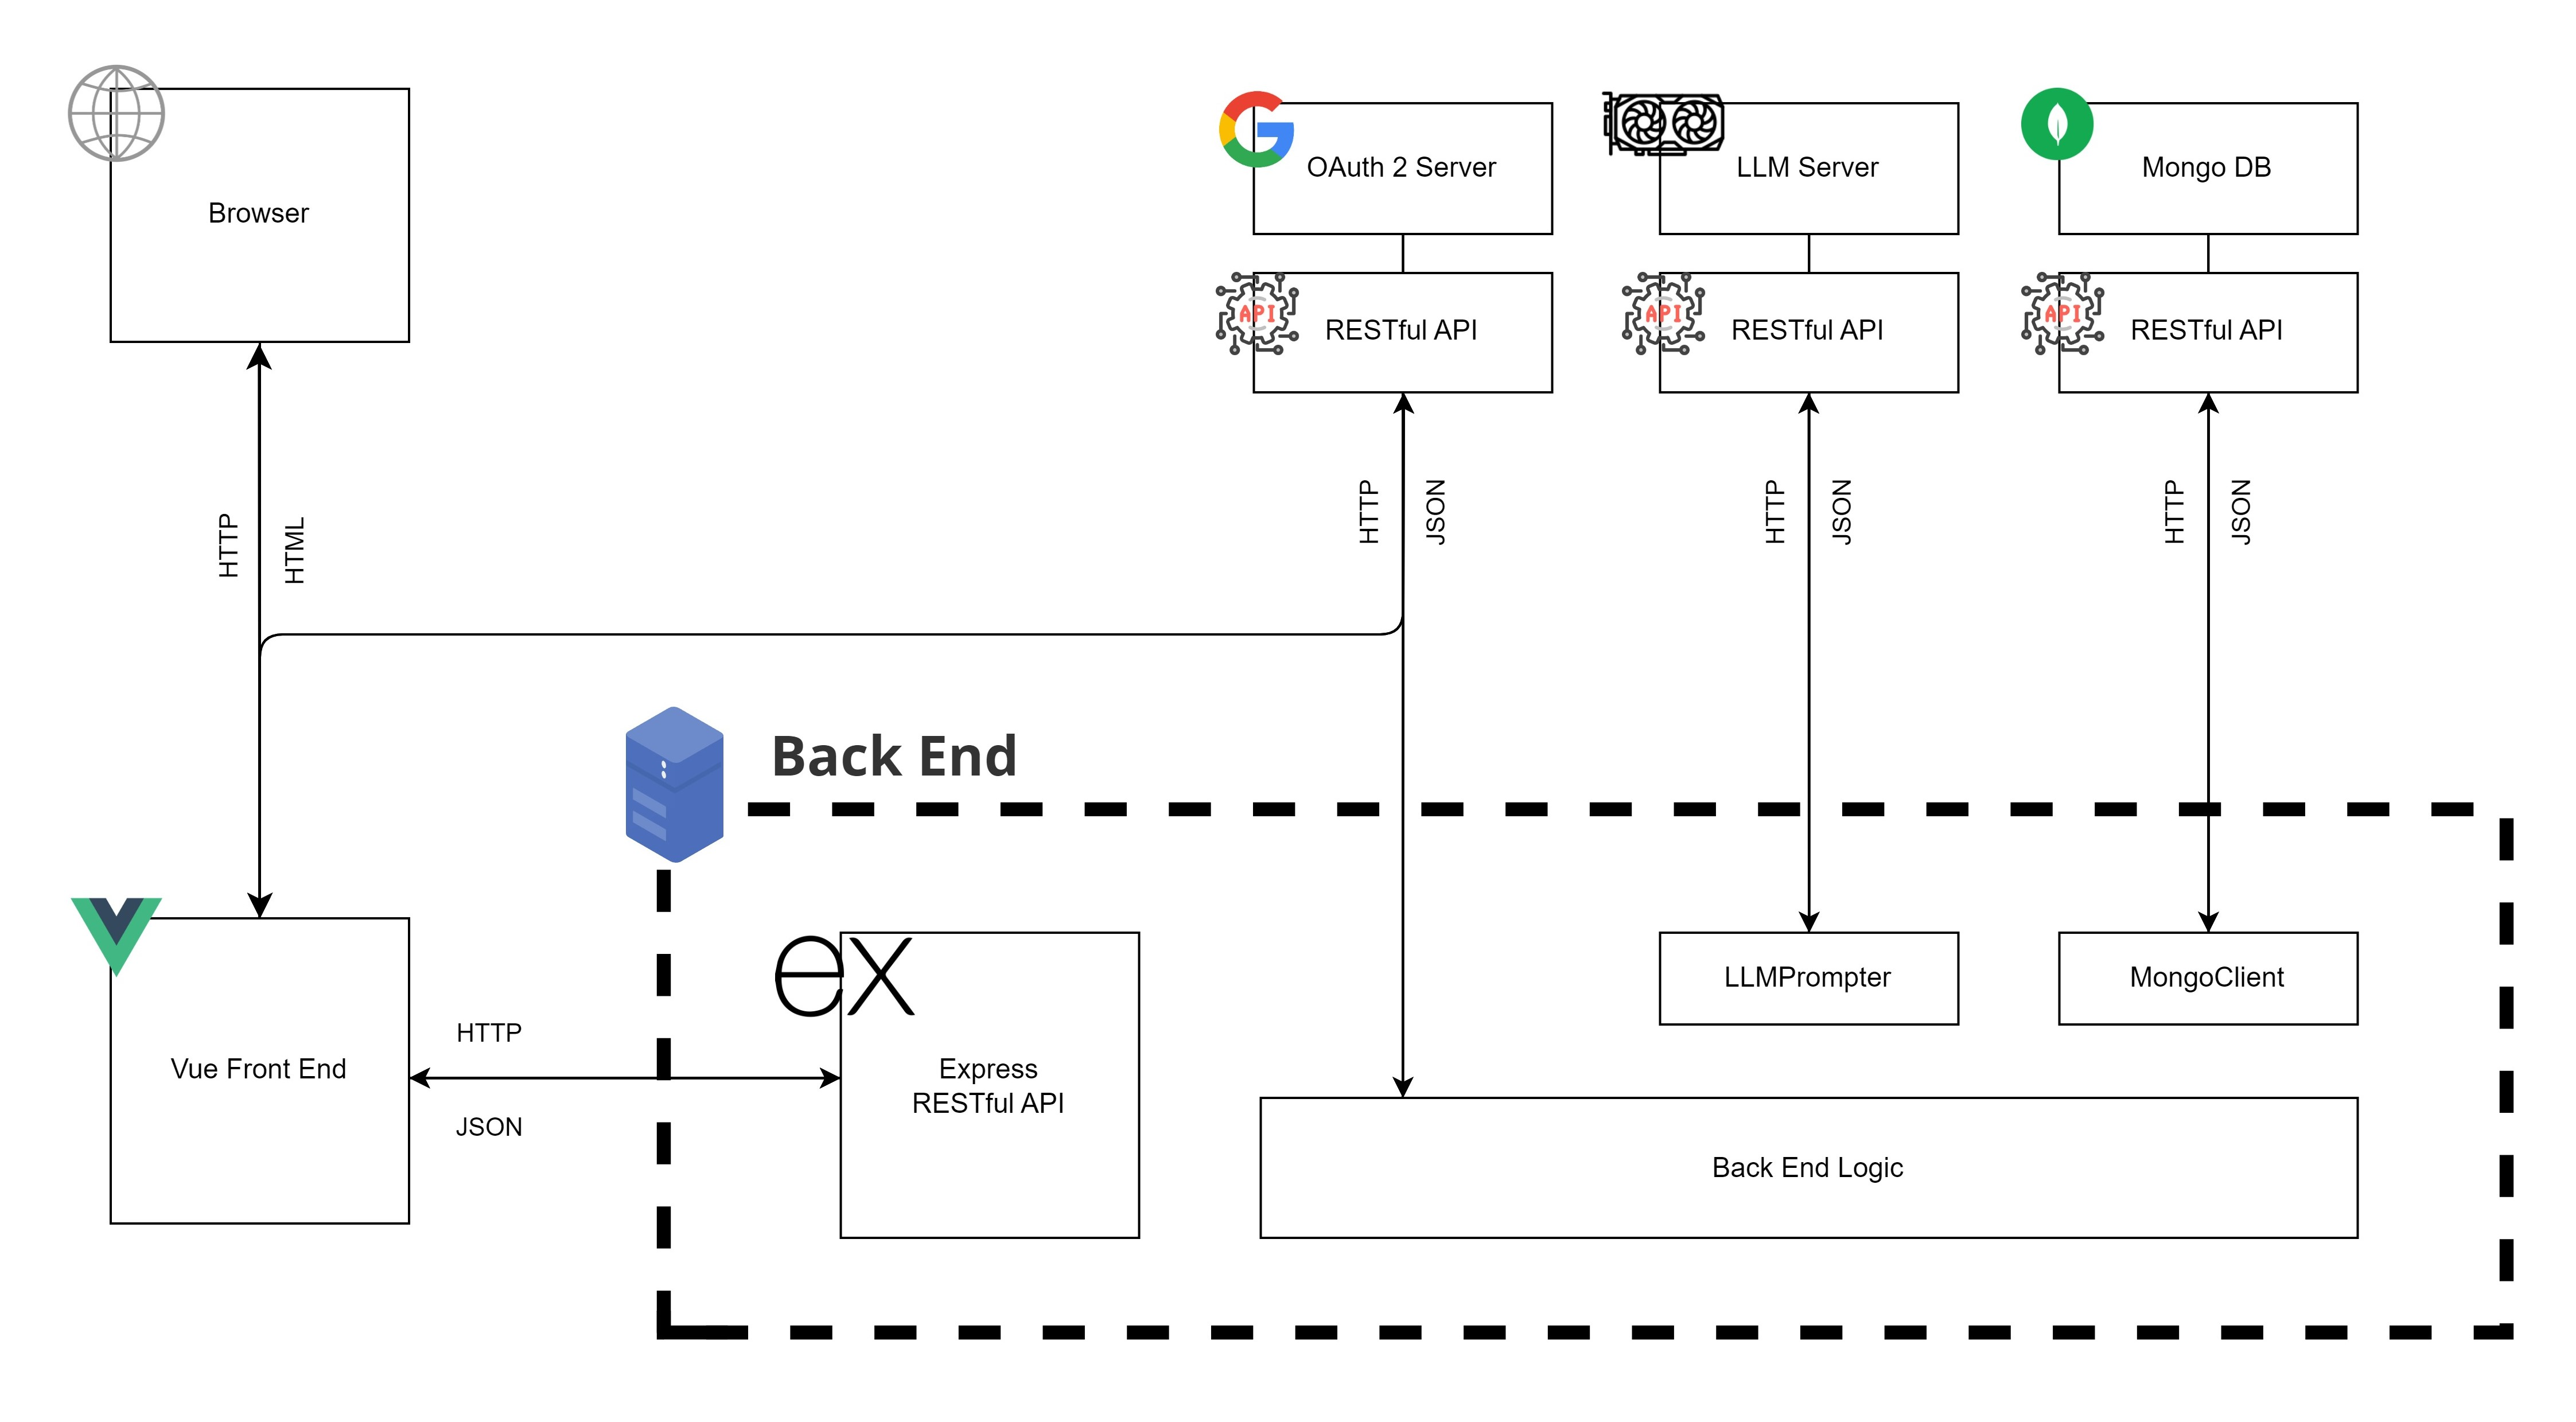
\includegraphics[width=0.95\textwidth]{images/architecture.jpg}
  \caption{\small The architecture diagram ot the MindMerge system}
\end{figure}
The architecture is relatively simple,
comprising two classical components: the front end and the back end, along with several smaller components (browser, OAuth server, LLM service, and MongoDB).
\newline \newline
The browser communicates with the front end using the HTTP protocol and HTML format.
\newline \newline
The front end, based on the Vue library, accesses resources provided by the back end using HTTP with JSON data format.
\newline \newline
Authentication is provided by a third-party OAuth server, that communicate with both the front end and back end via HTTP/JSON.
\newline \newline
The back end is the most complex component consists of several sub-components, including:
\begin{itemize}
  \item A part providing RESTful APIs based on Express.js
  \item A component dedicated to communicating with the database (MongoClient)
  \item A module for communicating with the LLM service (LLMPrompter)
  \item Logic containing all functions necessary for the application's operation.
\end{itemize}
All the communications that the backend has with the external world are made through HTTP with json format.
\newpage
\section{Product Backlog}

This section contains the product backlogs we have built during our development process.
There are a few differences between the various versions. The most obvious one is that we added a new colum
every time to represent the estimated effort that remained for every task. As well as some changes to the descriptions;
for example, we realized after we began the first sprint that we missed the ``so that..'' part of the user stories.
Therefore, we added it in the following versions.\newline
The complete list of all the product backlog we submitted, as well as the time they were written, is as follows:

\begin{itemize}
  \item \textbf{Version 1.0:} The initial product backlog, that was written before the sprint 1.
  \item \textbf{Version 2.0:} The second product backlog, tha was written between the sprint 1 and the sprint 2.
  \item \textbf{Version 3.0:} The third product backlog, that was written between the sprint 2 and the sprint 3.
  \item \textbf{Version 4.0:} The fourth product backlog, that was written at the end of the third sprint.
\end{itemize}
\subsection{Version 1.0}
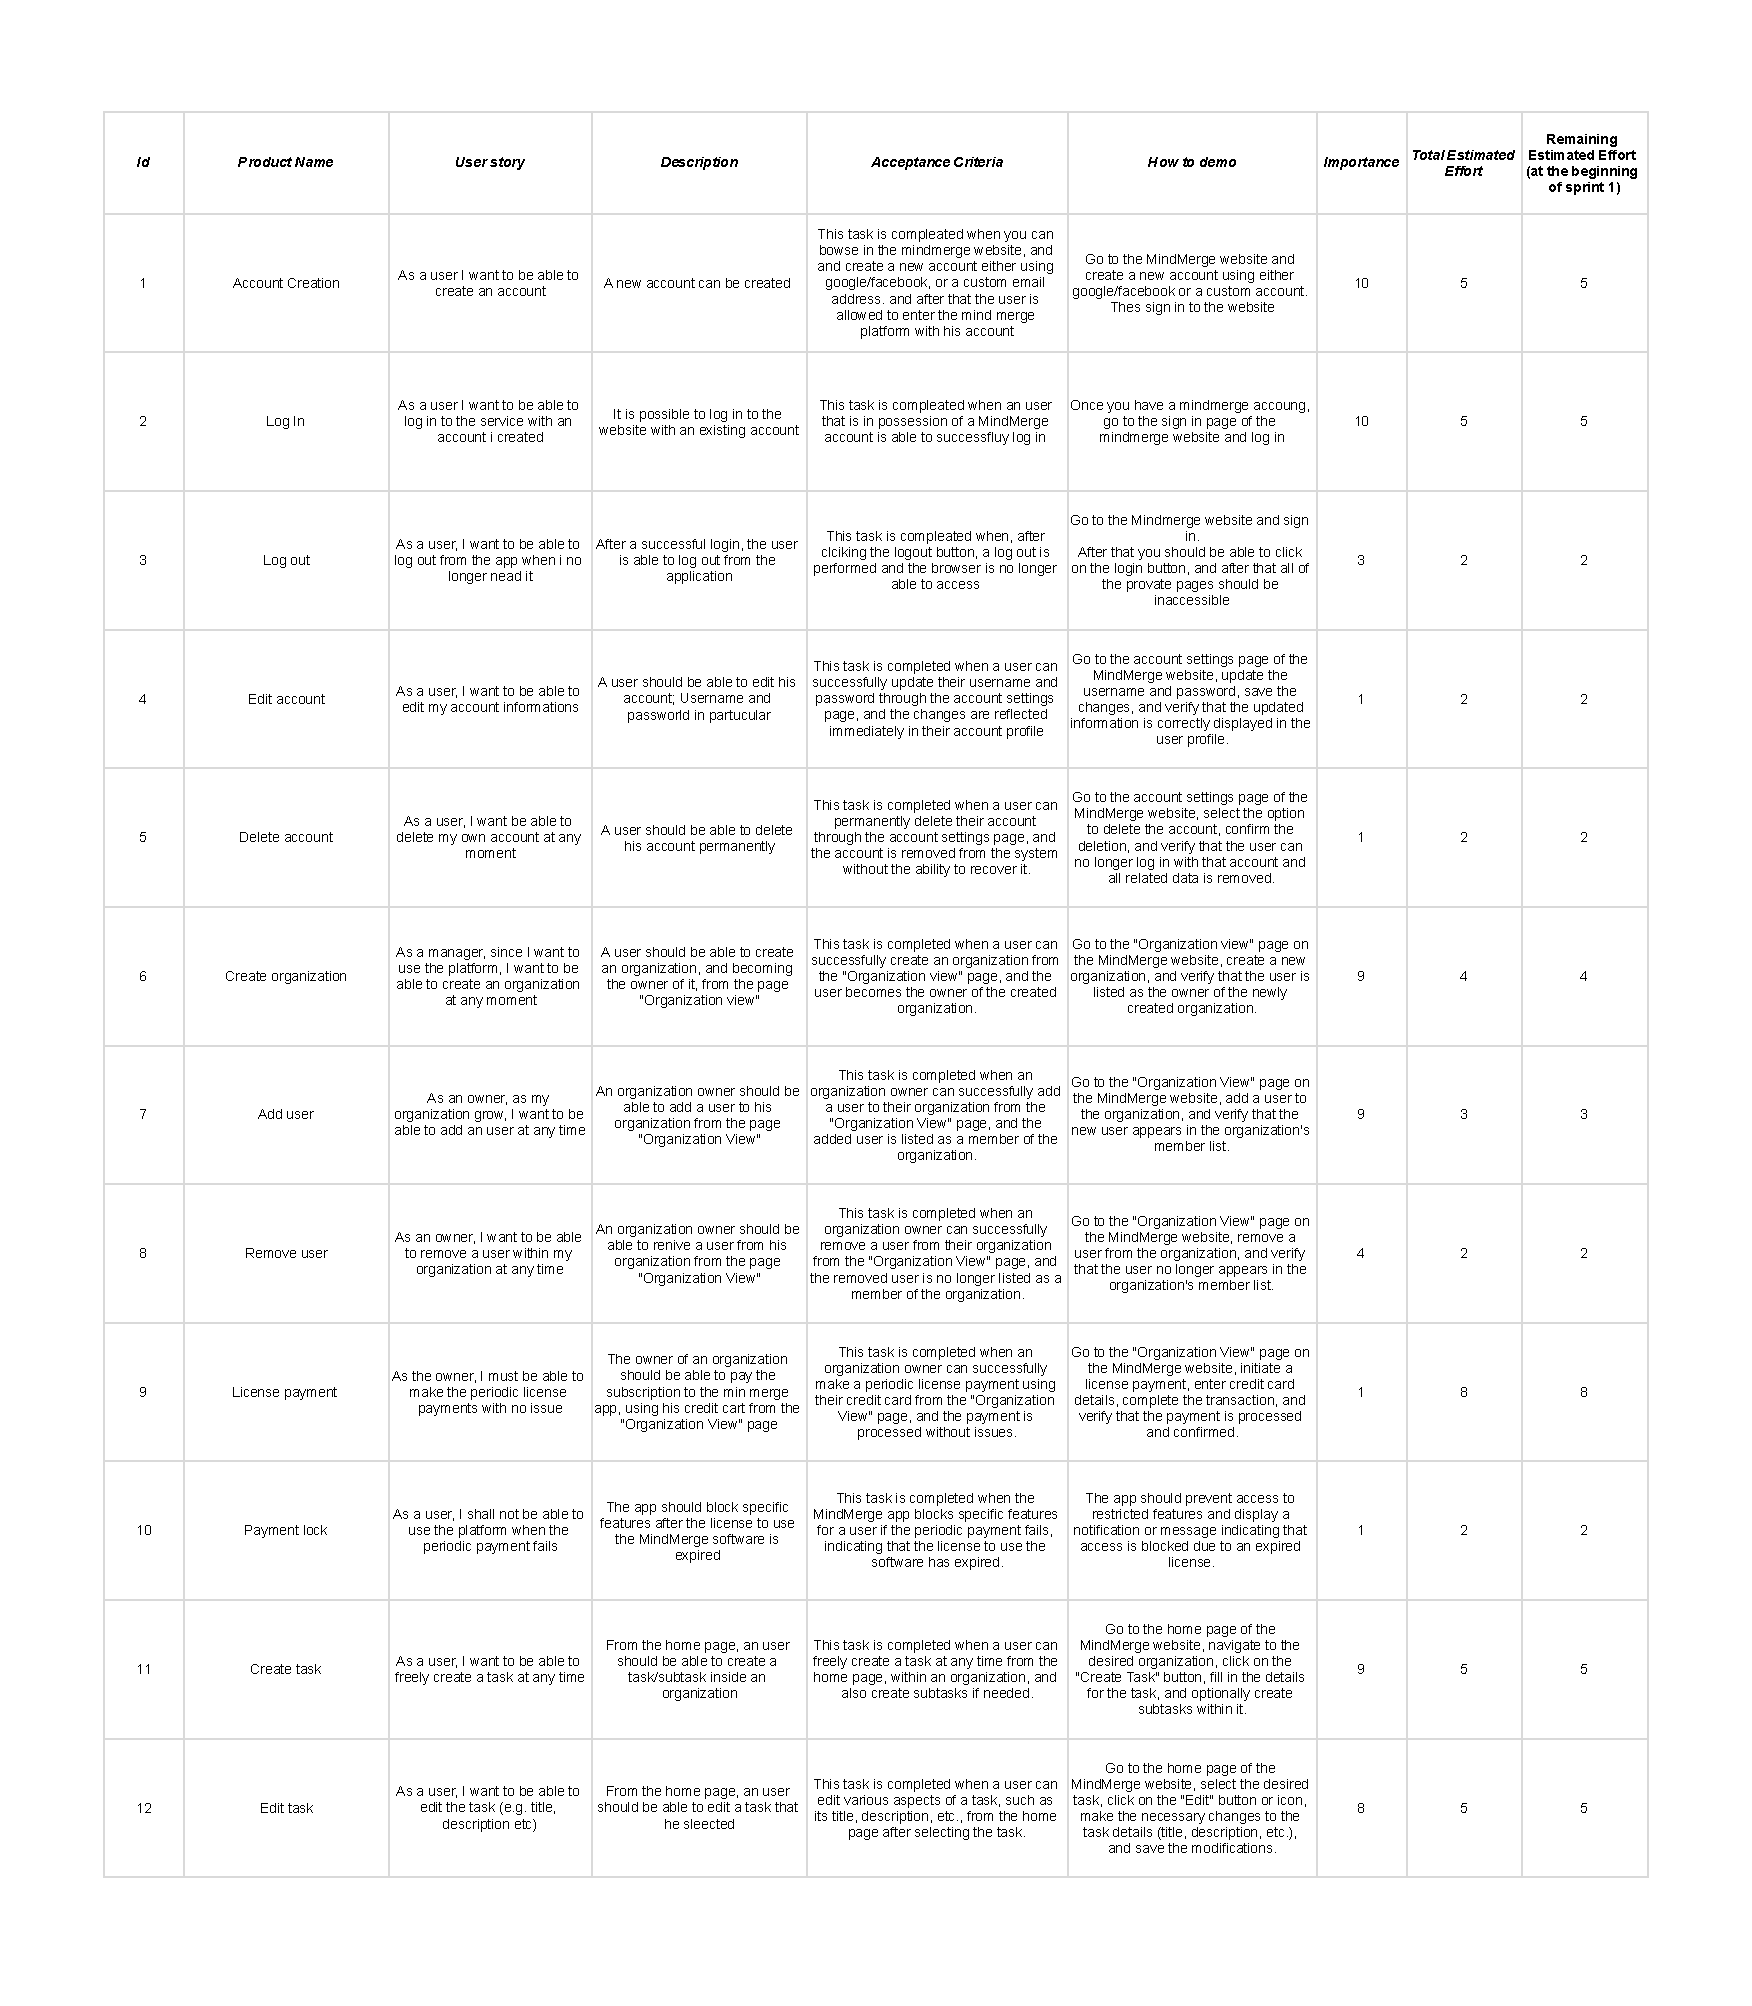
\includepdf[pages=-]{images/product_backlog_v1.pdf}
\subsection{Version 2.0}
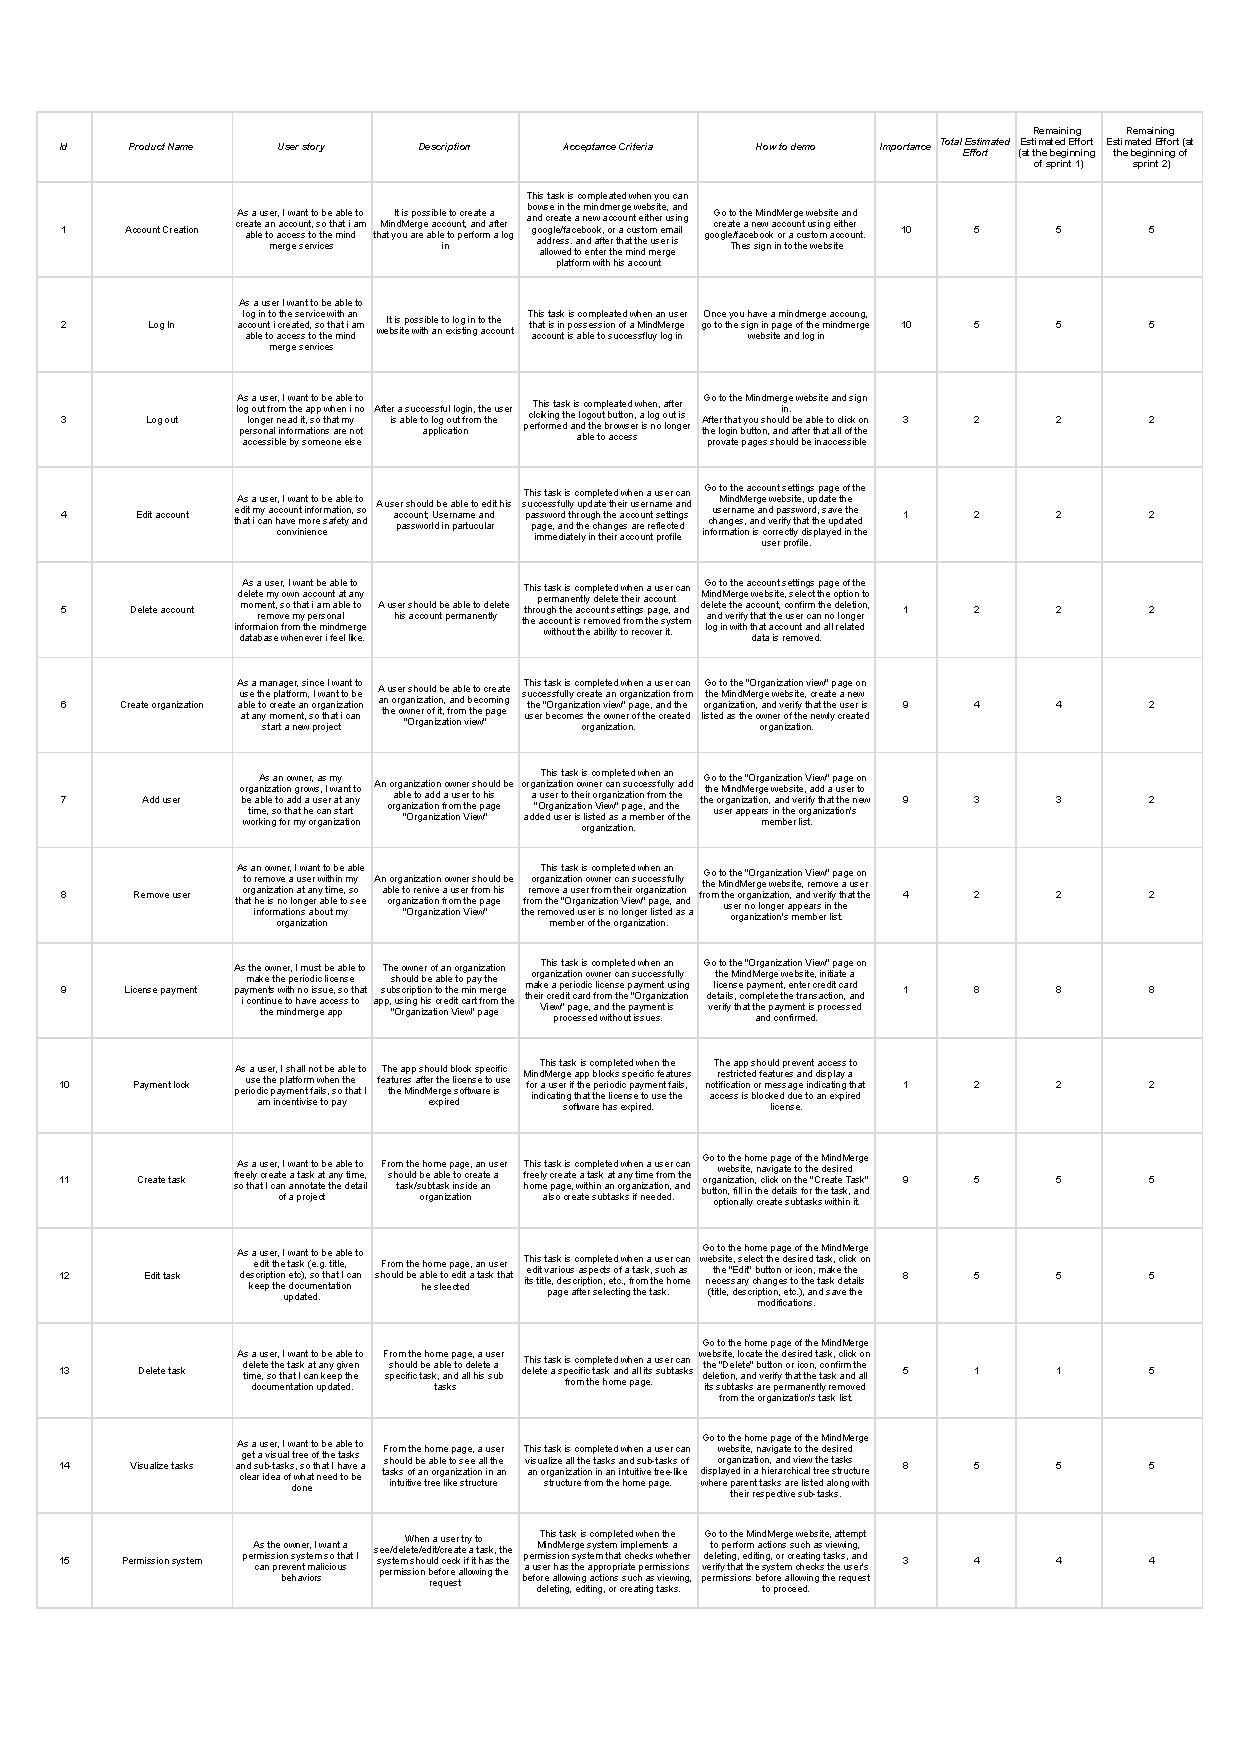
\includepdf[pages=-]{images/product_backlog_v2.pdf}
\subsection{Version 3.0}
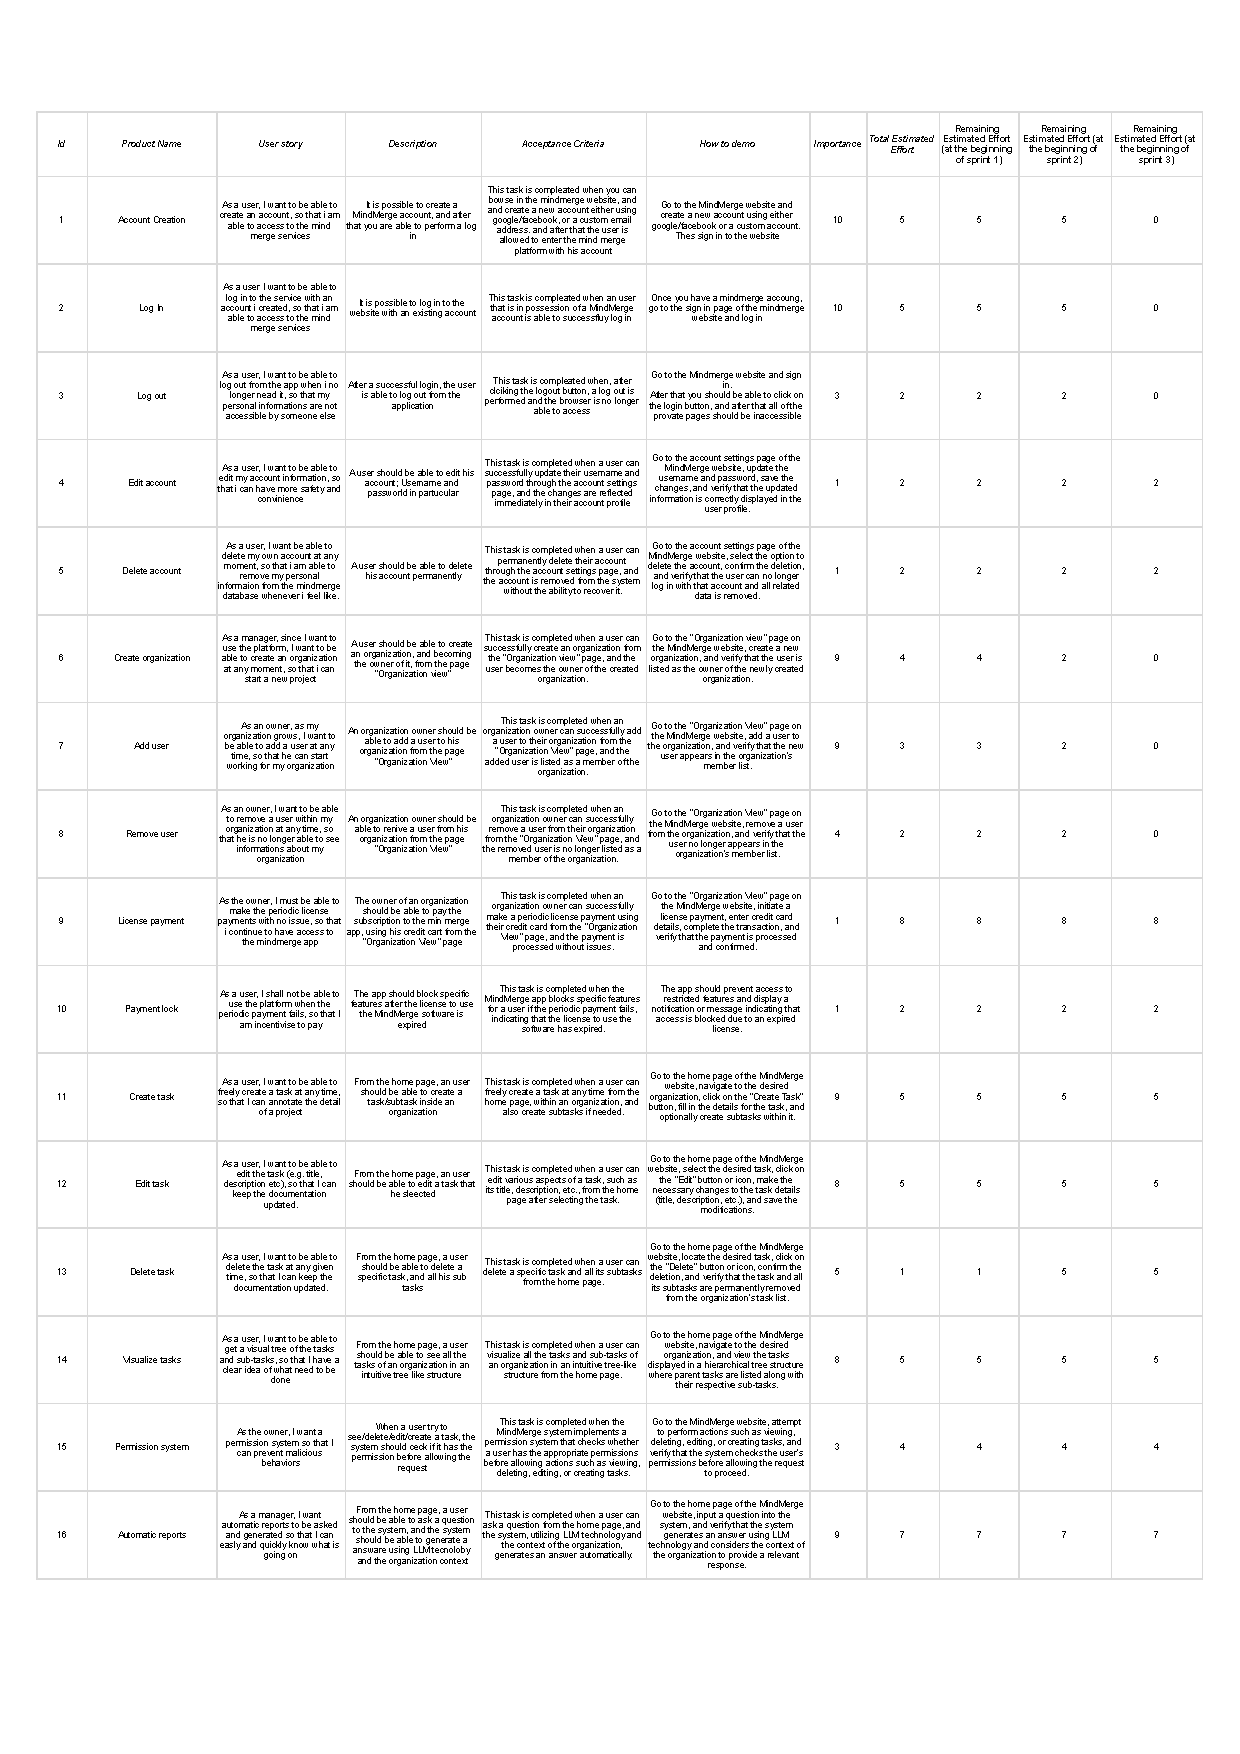
\includepdf[pages=-]{images/product_backlog_v3.pdf}
\subsection{Version 4.0}
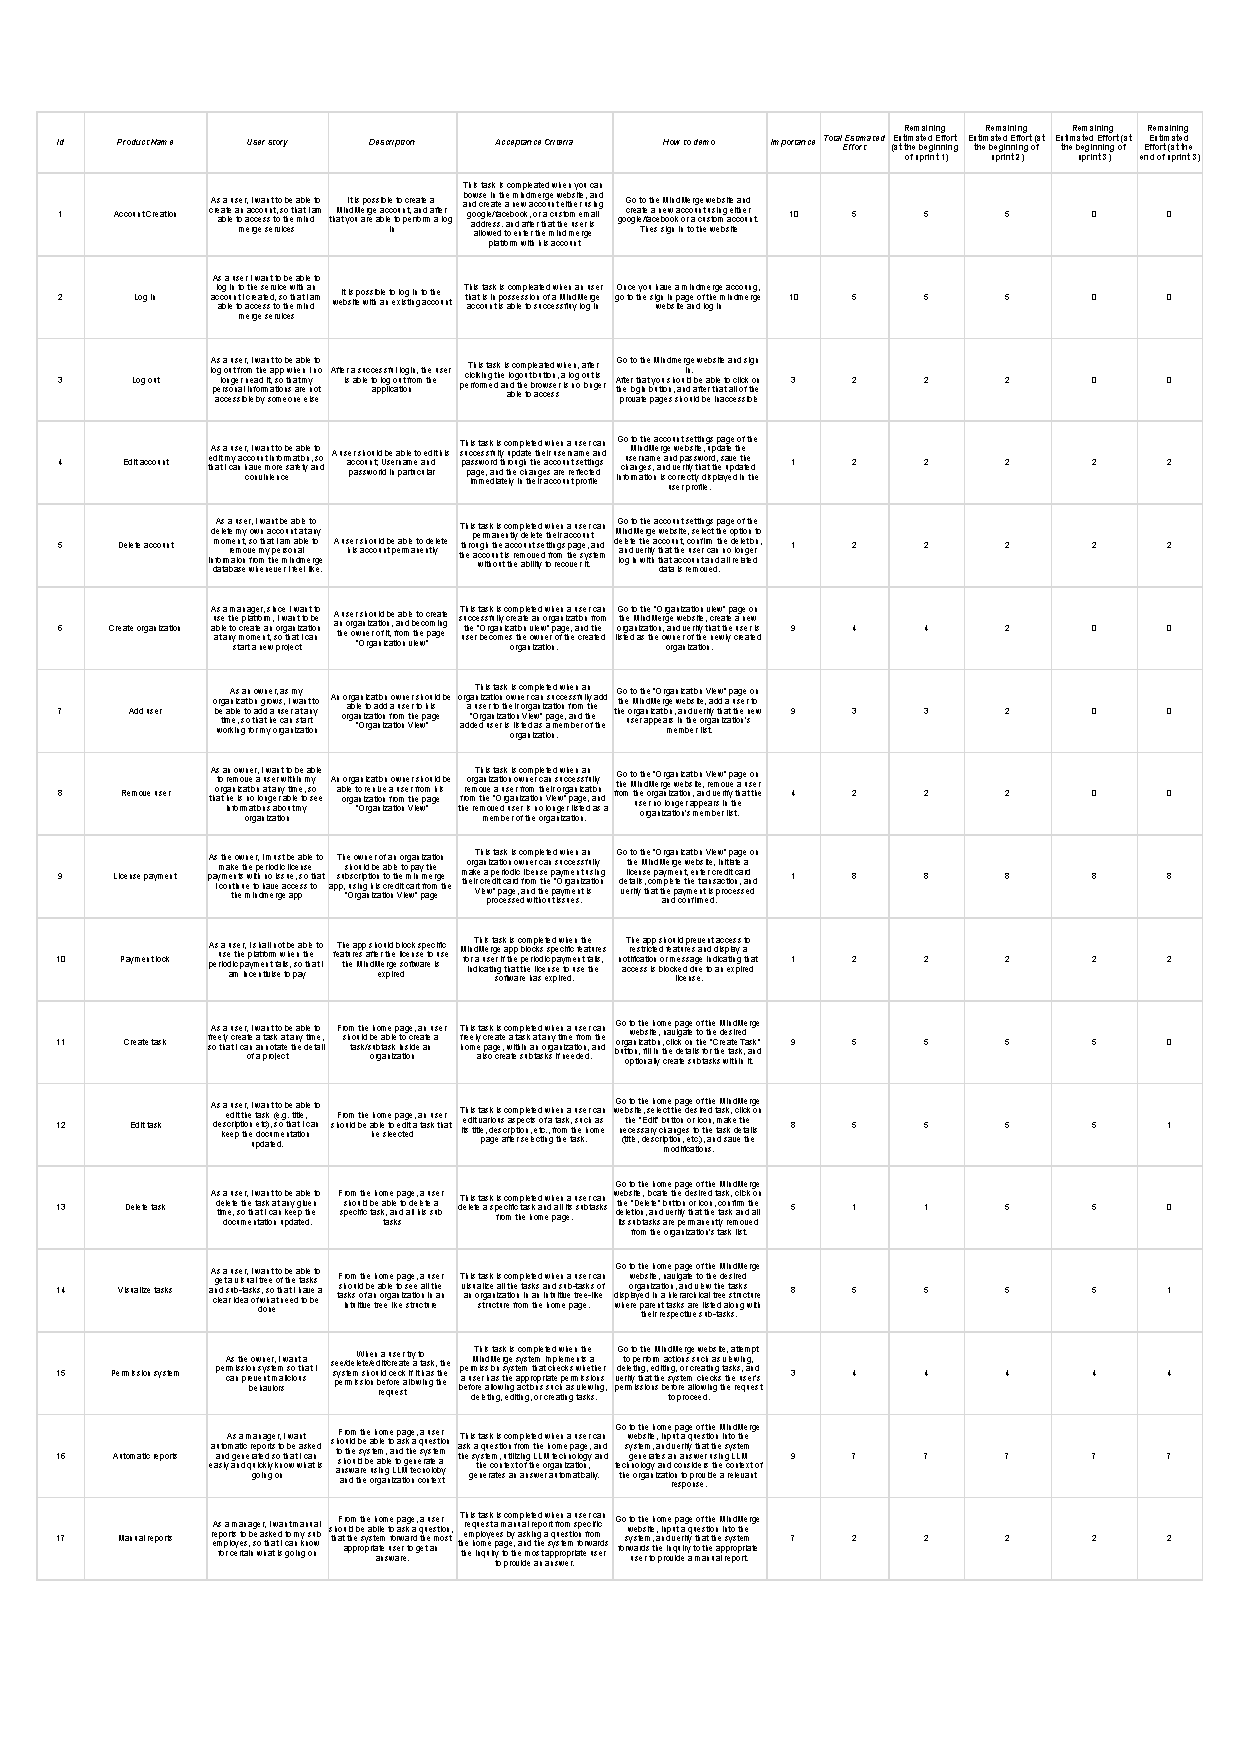
\includepdf[pages=-]{images/product_backlog_v4.pdf}

\section{Definition of Tests}

\subsection*{Test DatabaseManager:TaskManager}
This section contains the tests for the TaskManager class, which is responsible for managing tasks in the database.
\newline
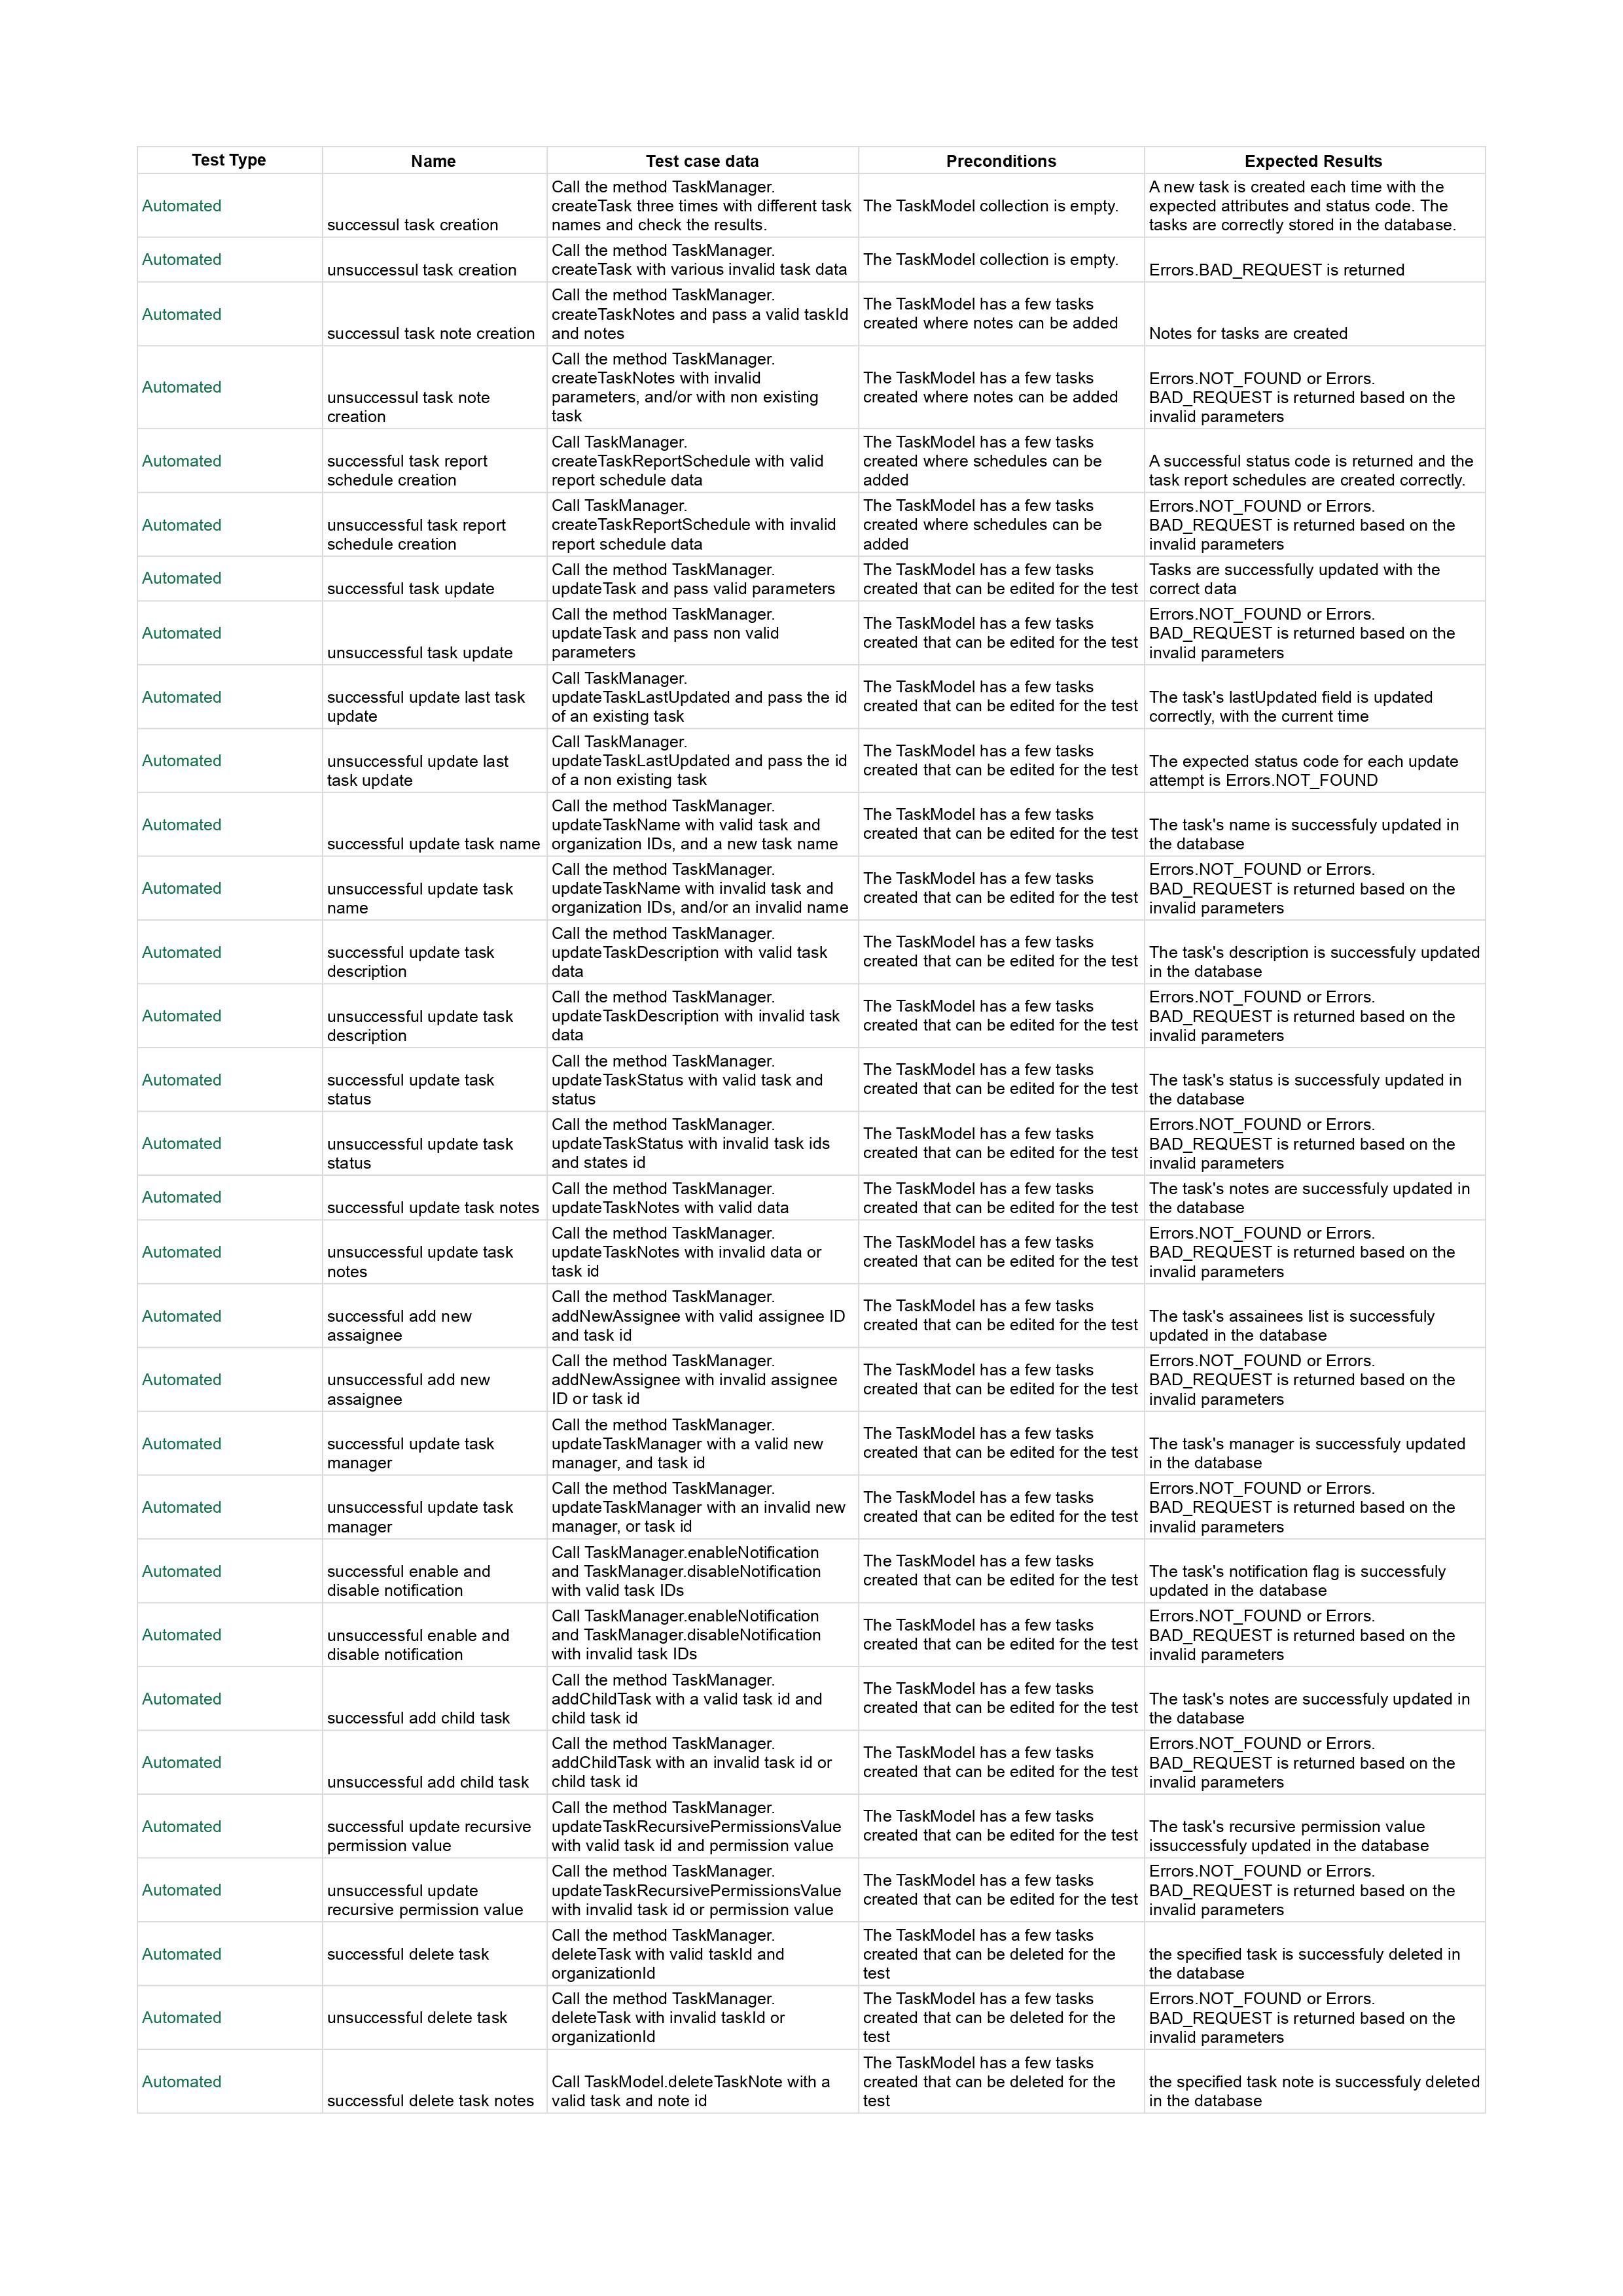
\includegraphics[width=0.95\textwidth]{images/Test_DatabaseManagerTaskManager-immagini-0.jpg}
\newline
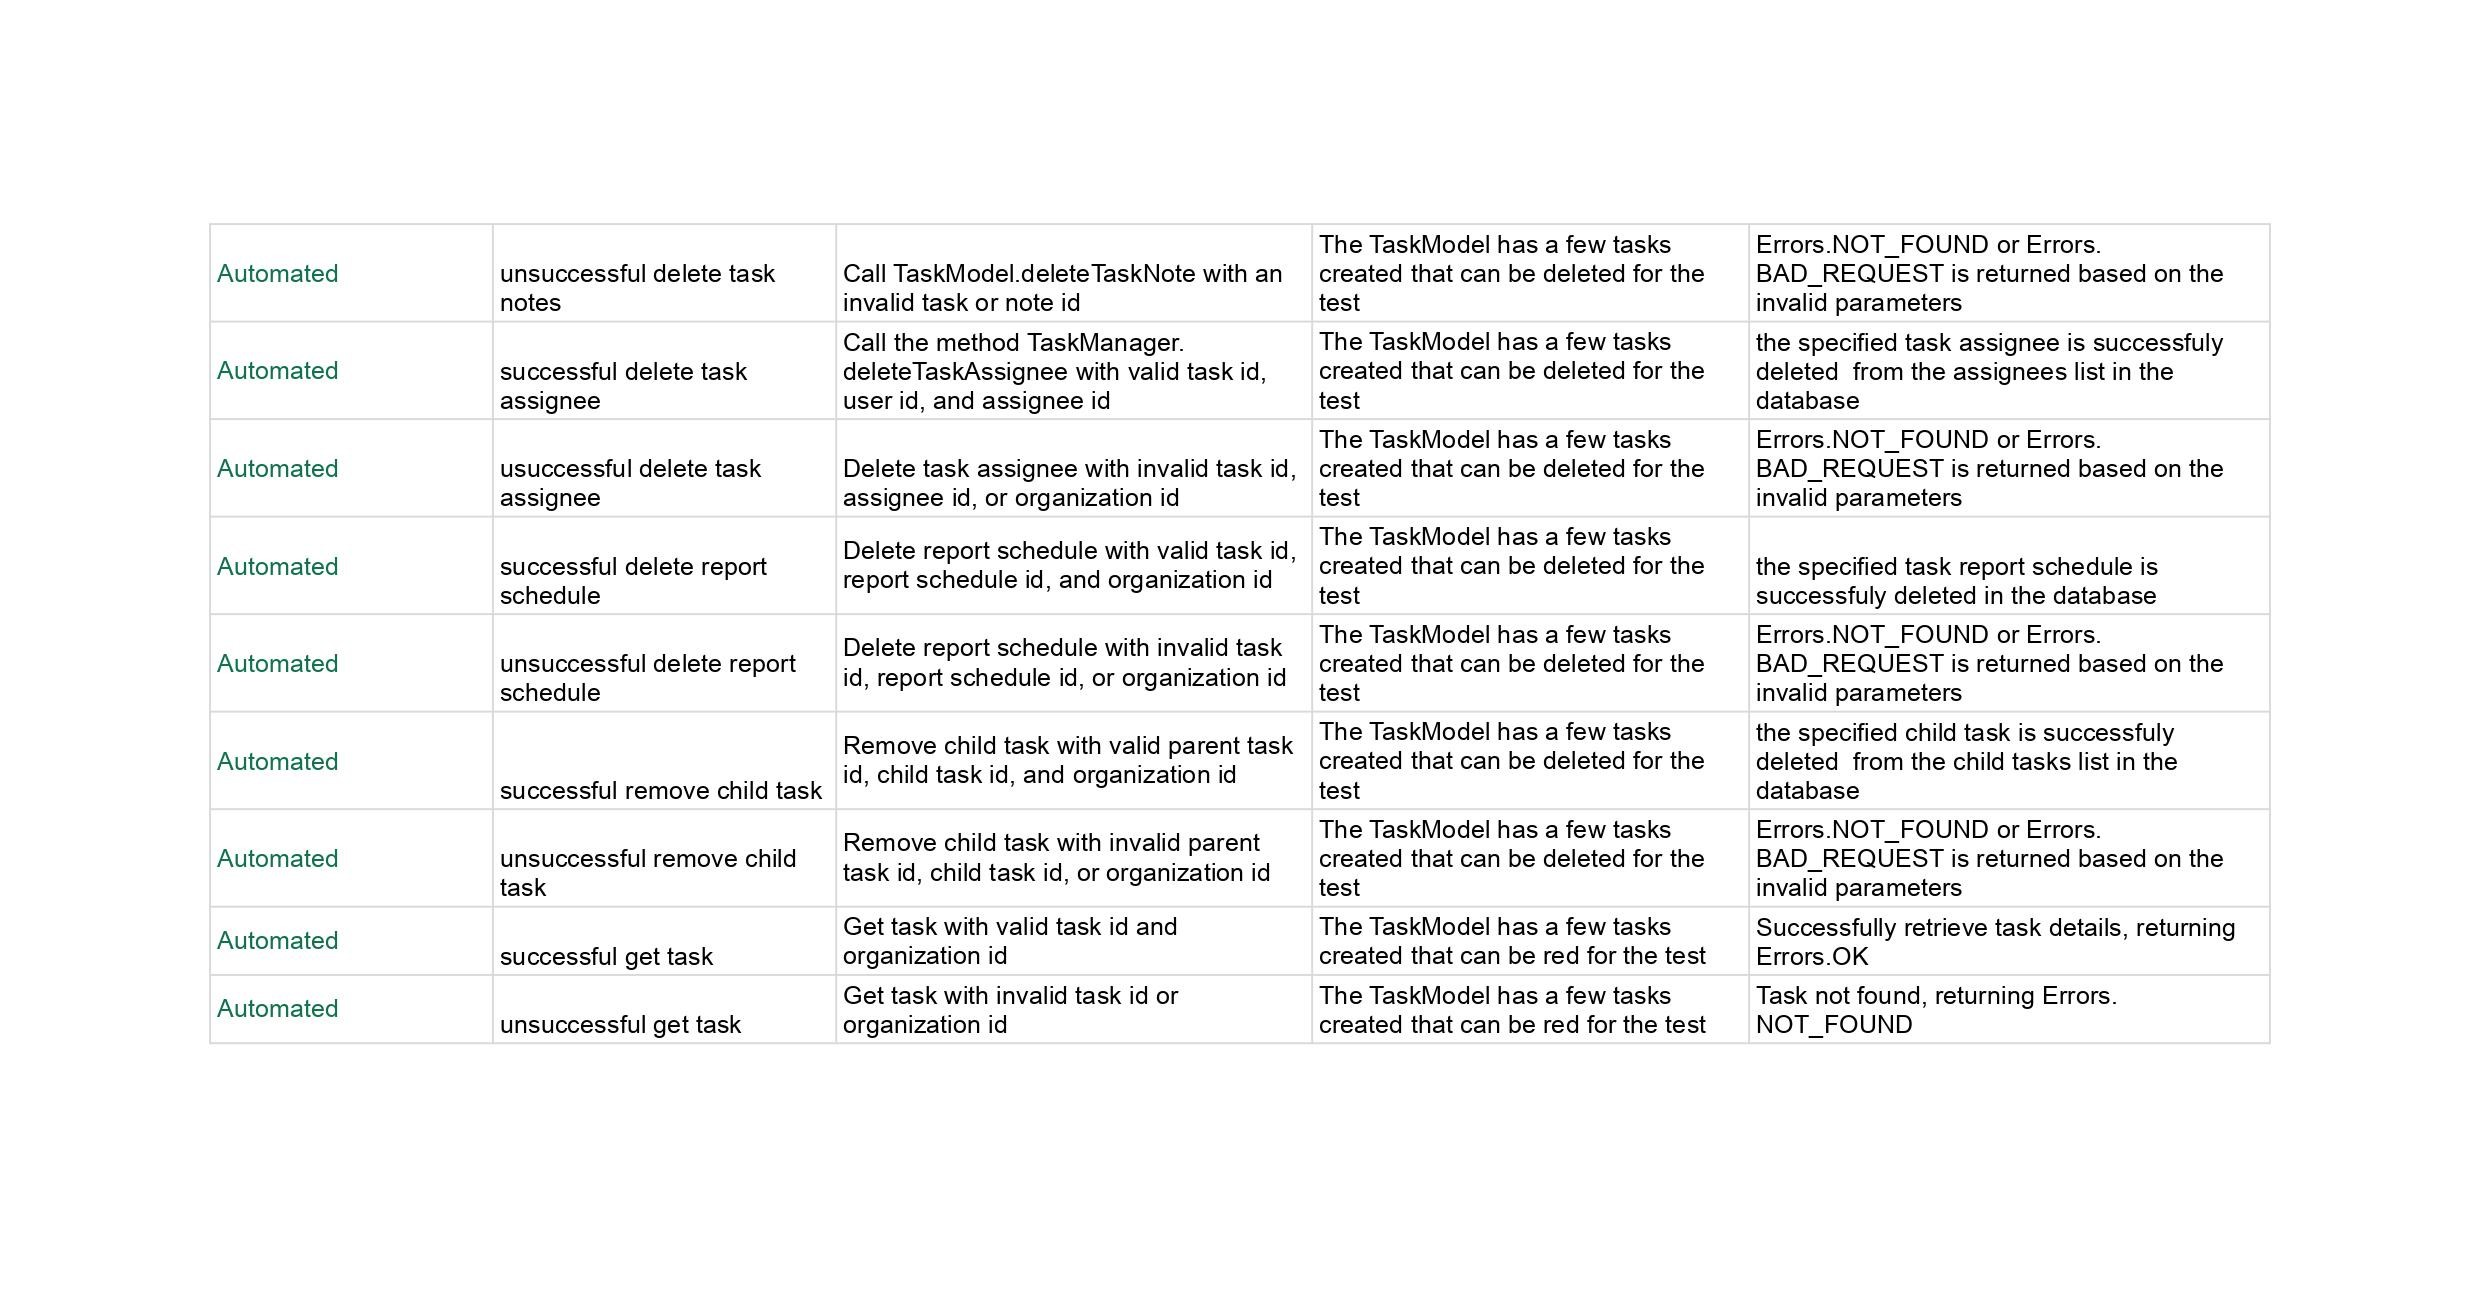
\includegraphics[width=0.95\textwidth]{images/Test_DatabaseManagerTaskManager-immagini-1.jpg}
\subsection*{Test OrganizationManager}
This section is dedicated to the tests for the OrganizationManager class, which is responsible for managing organizations in the database, with the integrated API.
\newline
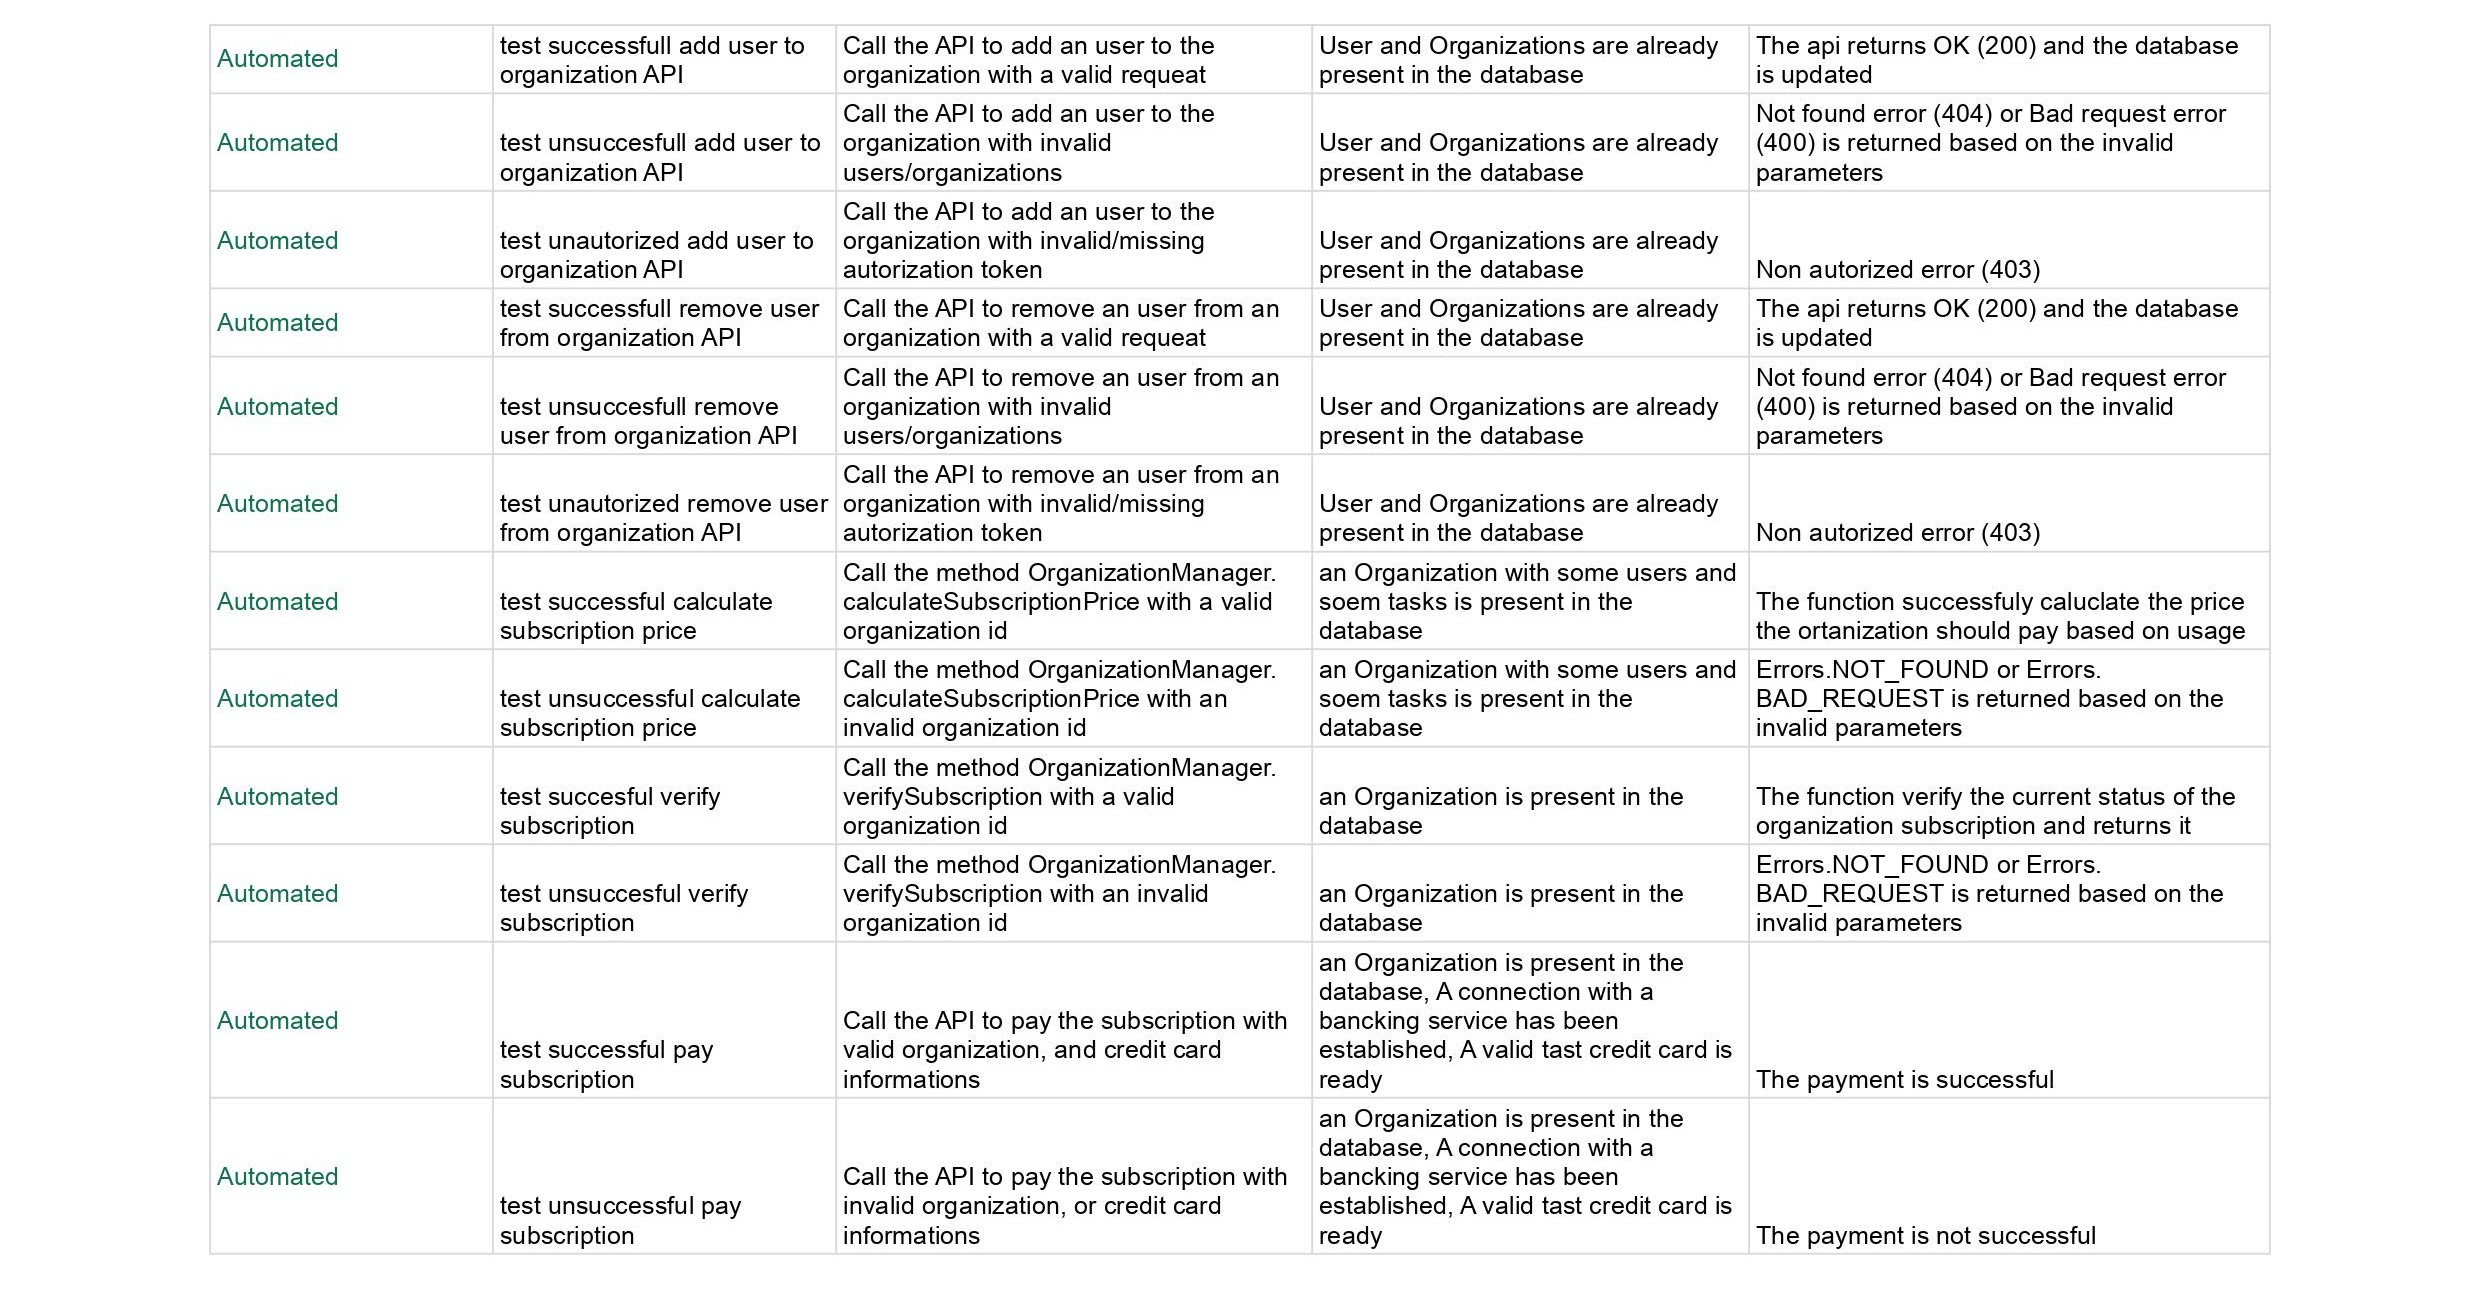
\includegraphics[width=0.95\textwidth]{images/Test_OrganizationManager.jpg}

\subsection*{Test Report Page}
This section includes manual tests for the Report Page, which is responsible for generating reports.
\newline
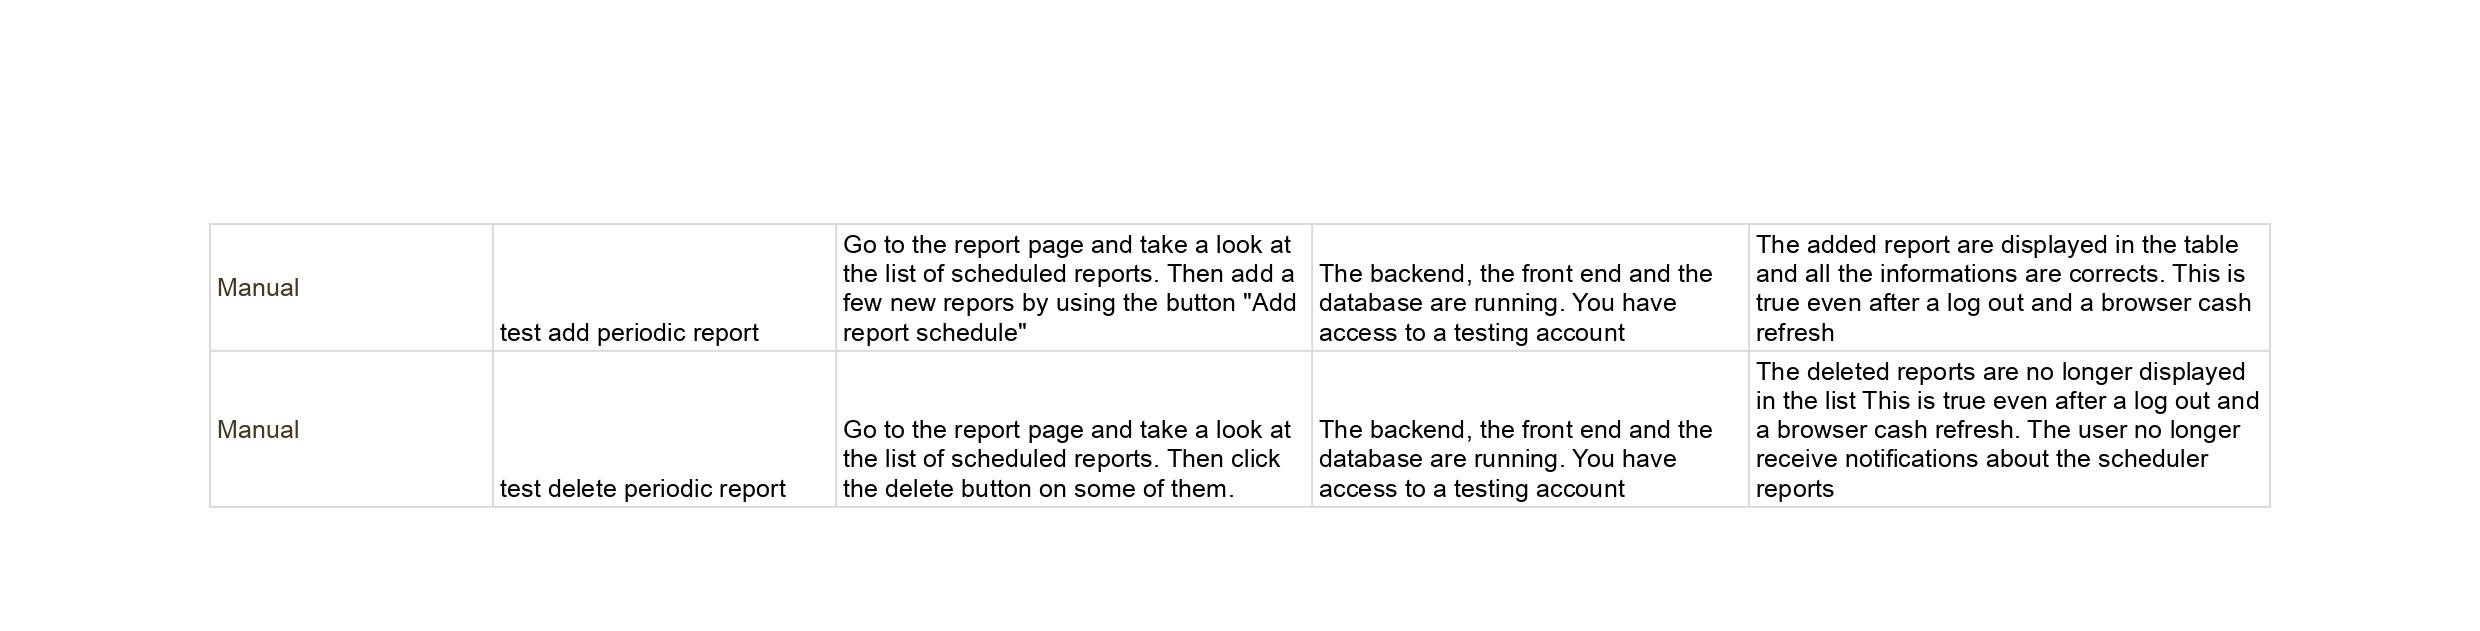
\includegraphics[width=0.95\textwidth]{images/Test_ReportPage.jpg}
\subsection*{Test NotificationManager}
This section includes automated tests for the NotificationManager class, which is responsible for managing notifications in the database.
\newline
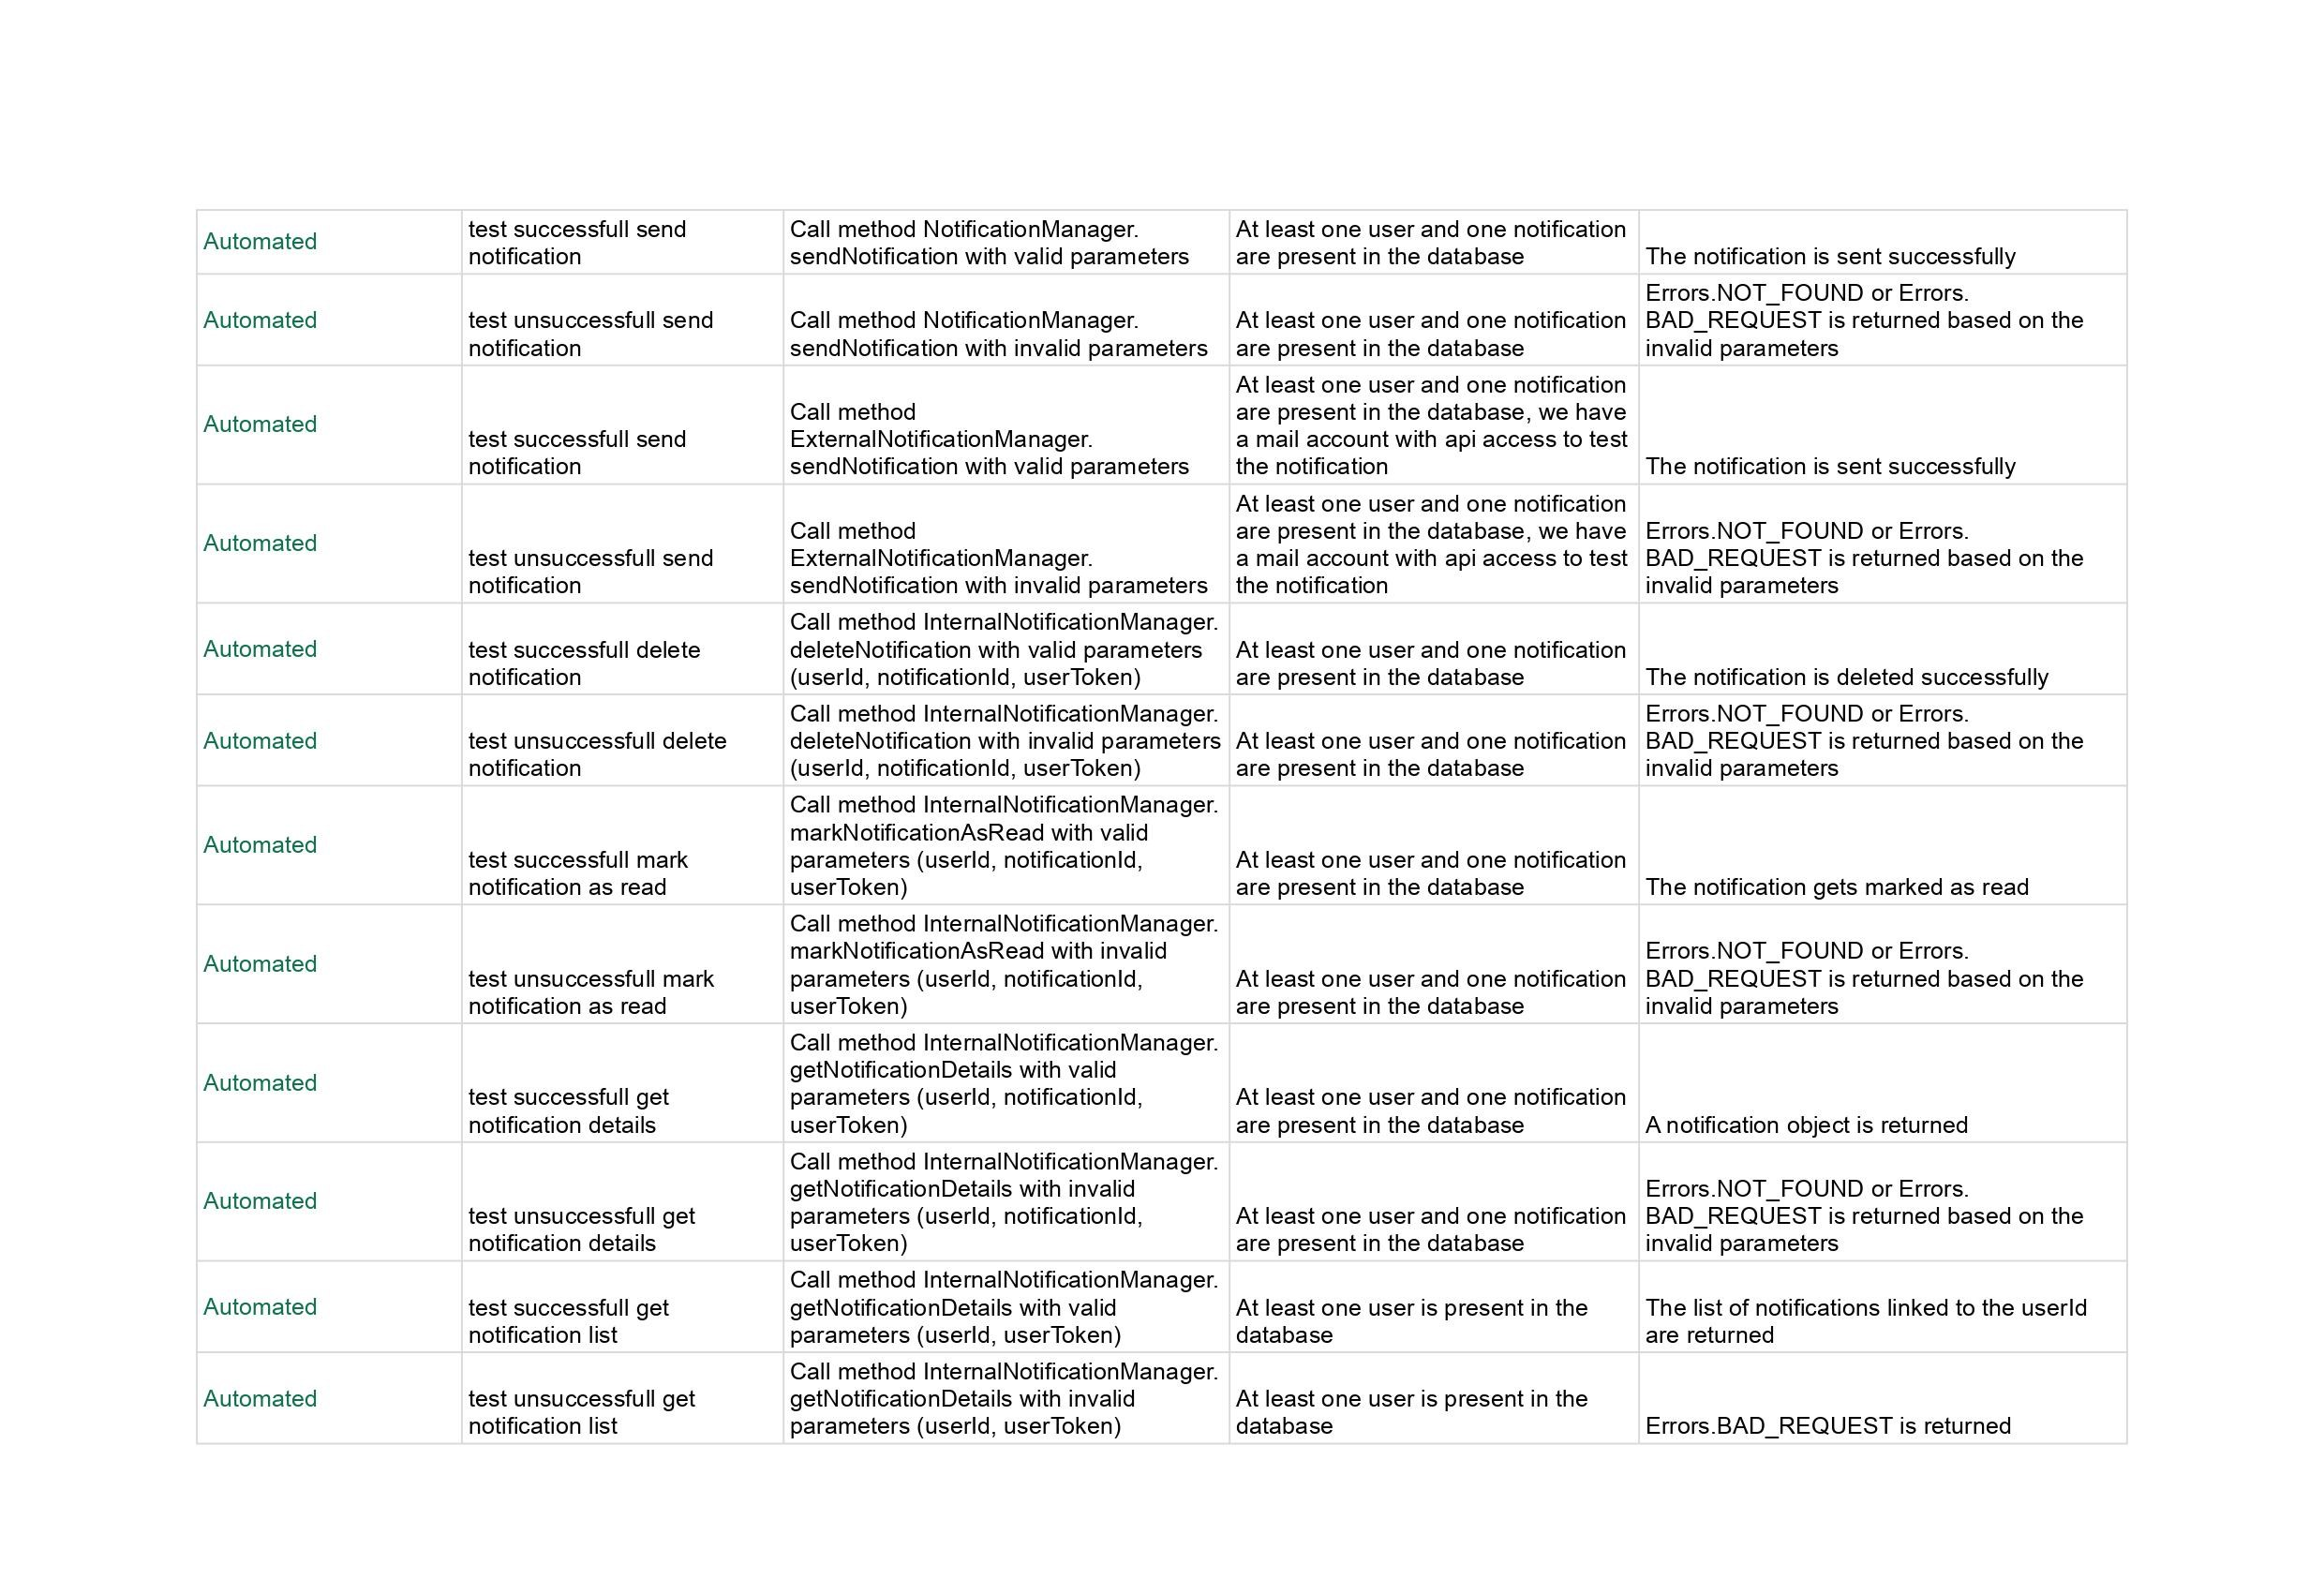
\includegraphics[width=0.95\textwidth]{images/Test_NotificationManager.jpg}

\subsection*{Test ReportManager}
This section includes automated tests for the ReportManager class, which is responsible for managing reports in the database.
\newline
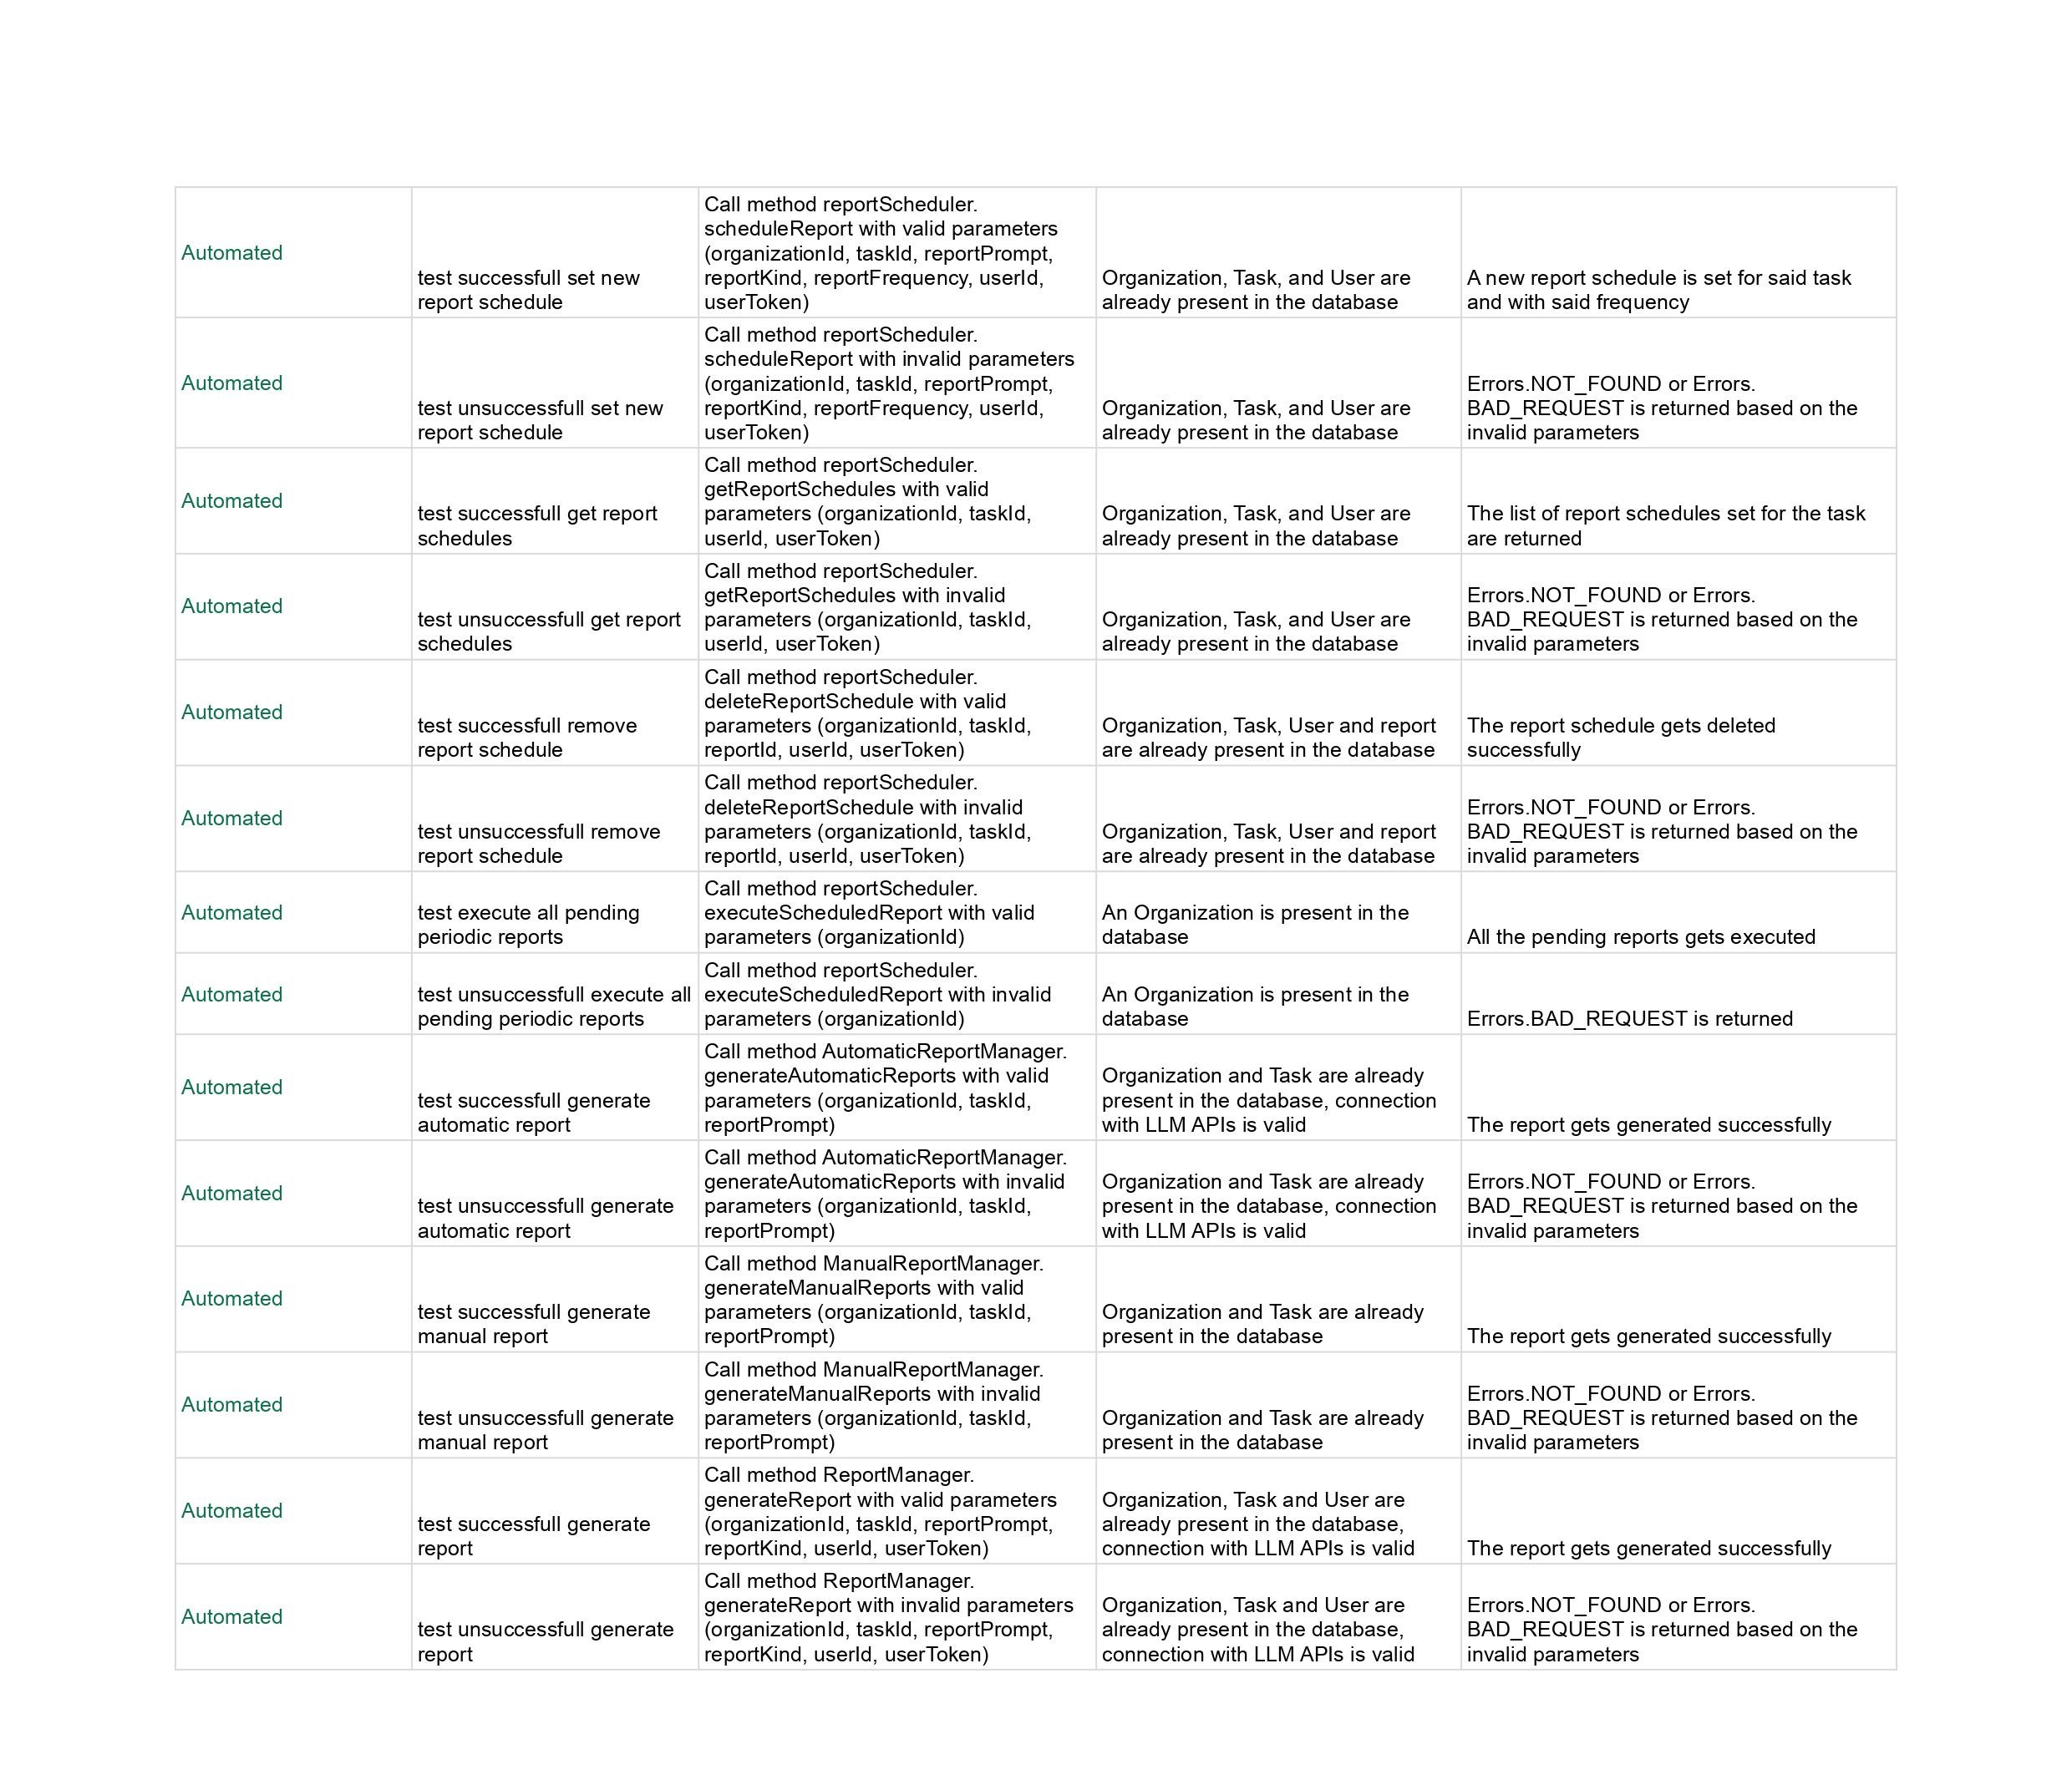
\includegraphics[width=0.95\textwidth]{images/Test_ReportManager.jpg}

\subsection*{Test DatabaseManager::OrganizationManager}
This section is dedicated to the tests for the OrganizationManager class, which is responsible for managing organizations in the database.
\newline
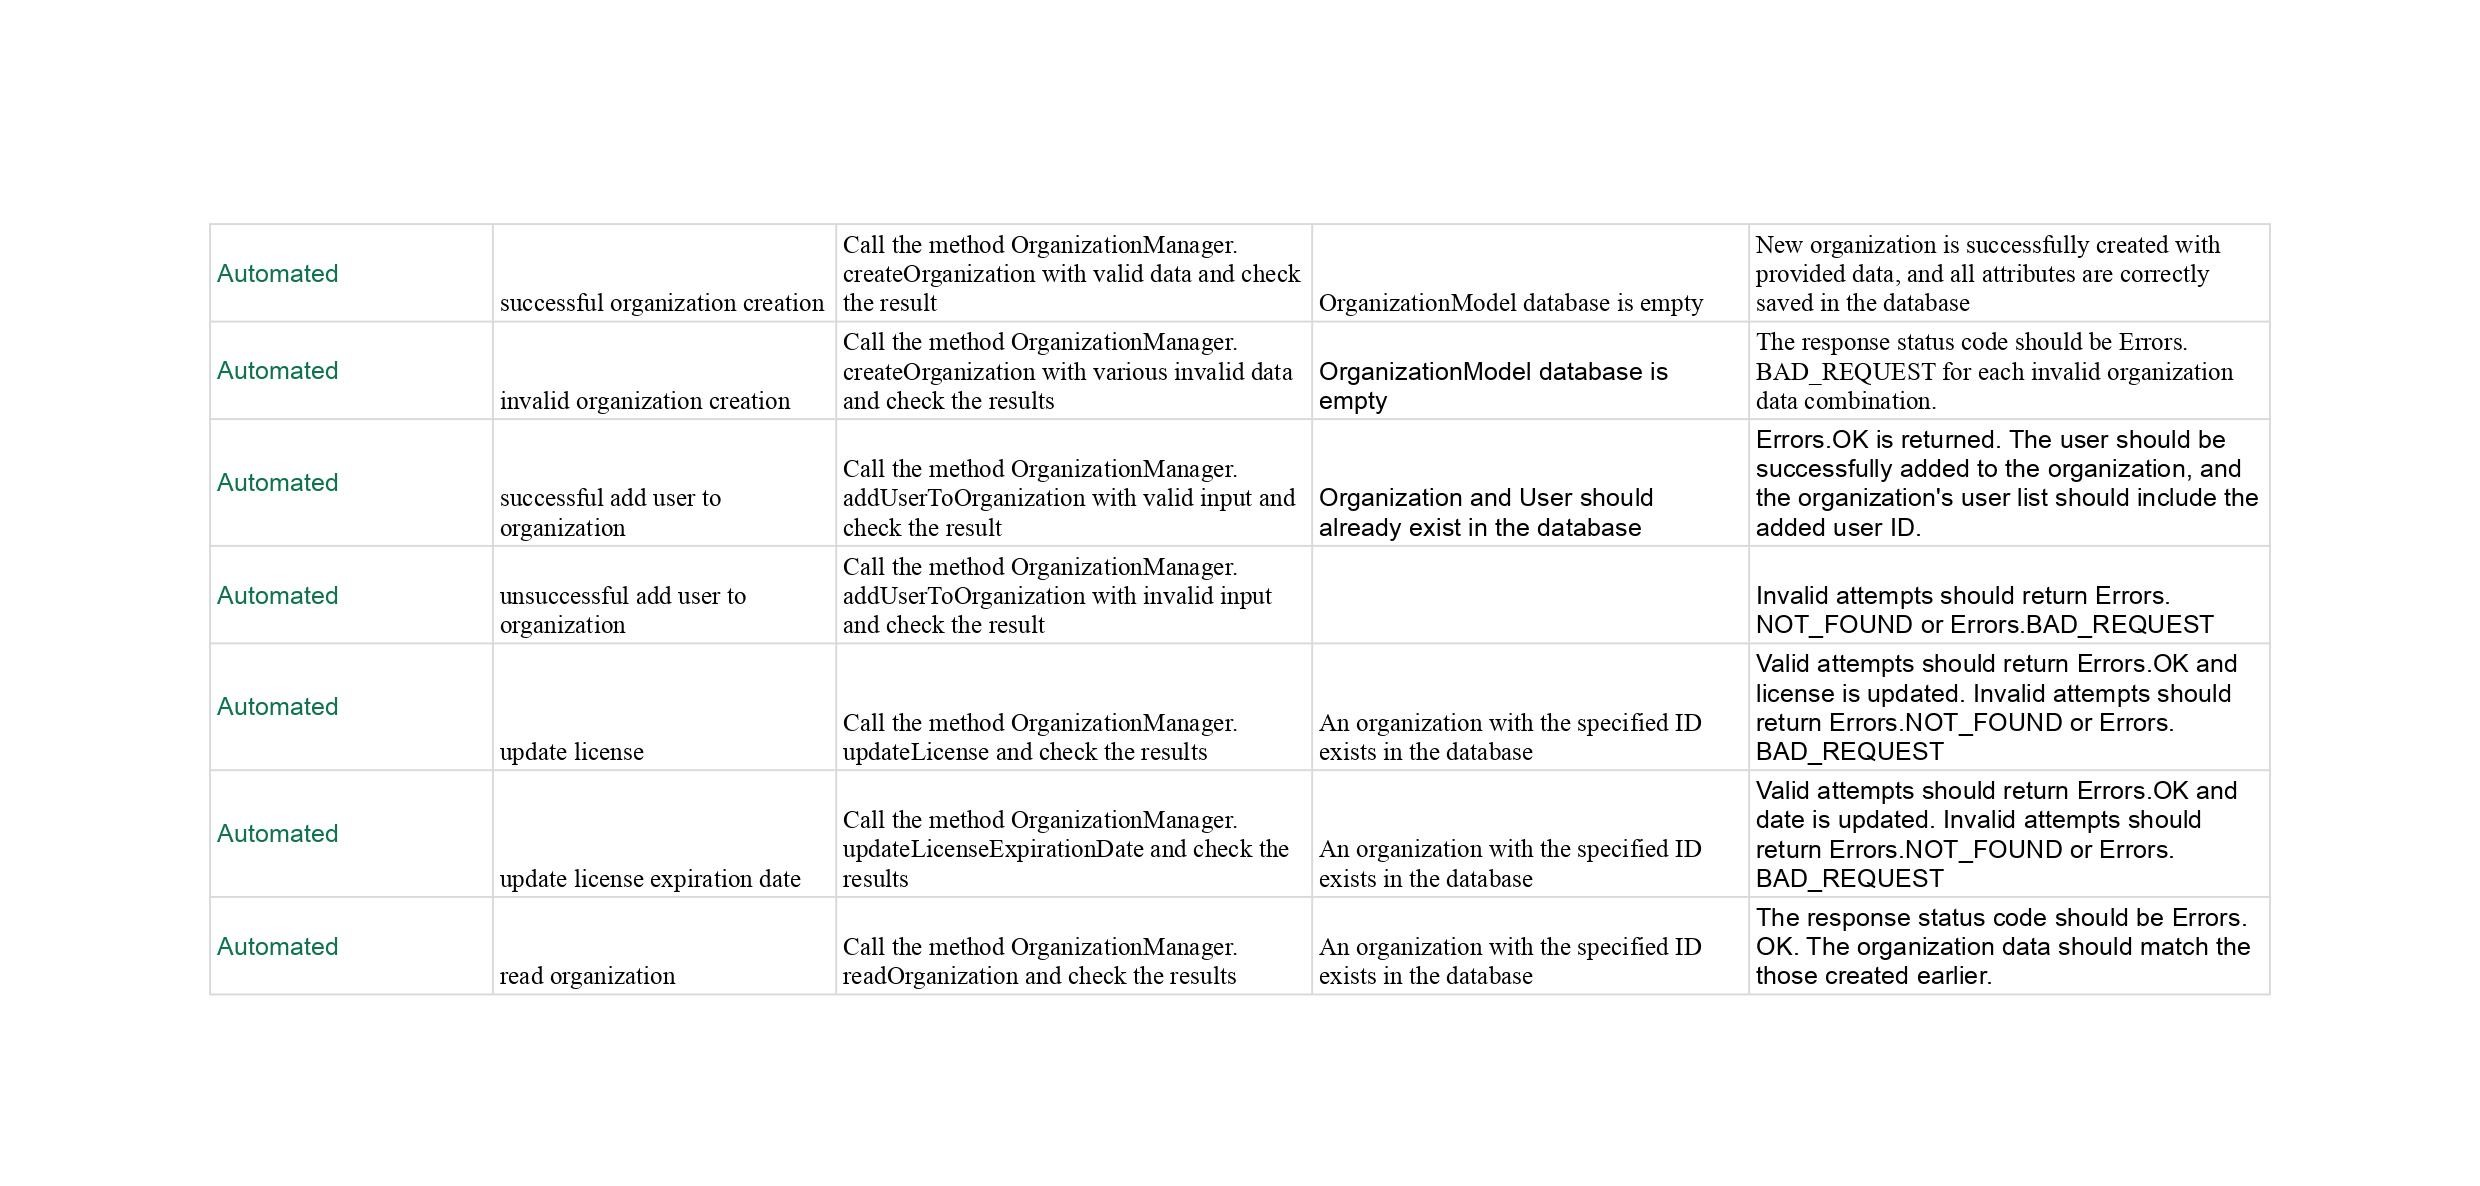
\includegraphics[width=0.95\textwidth]{images/Test_DatabaseManagerOrganizationManager.jpg}

\subsection*{Test AccountManager}
This section includes automated tests for the AccountManager class, which is responsible for managing accounts in the database.
\newline
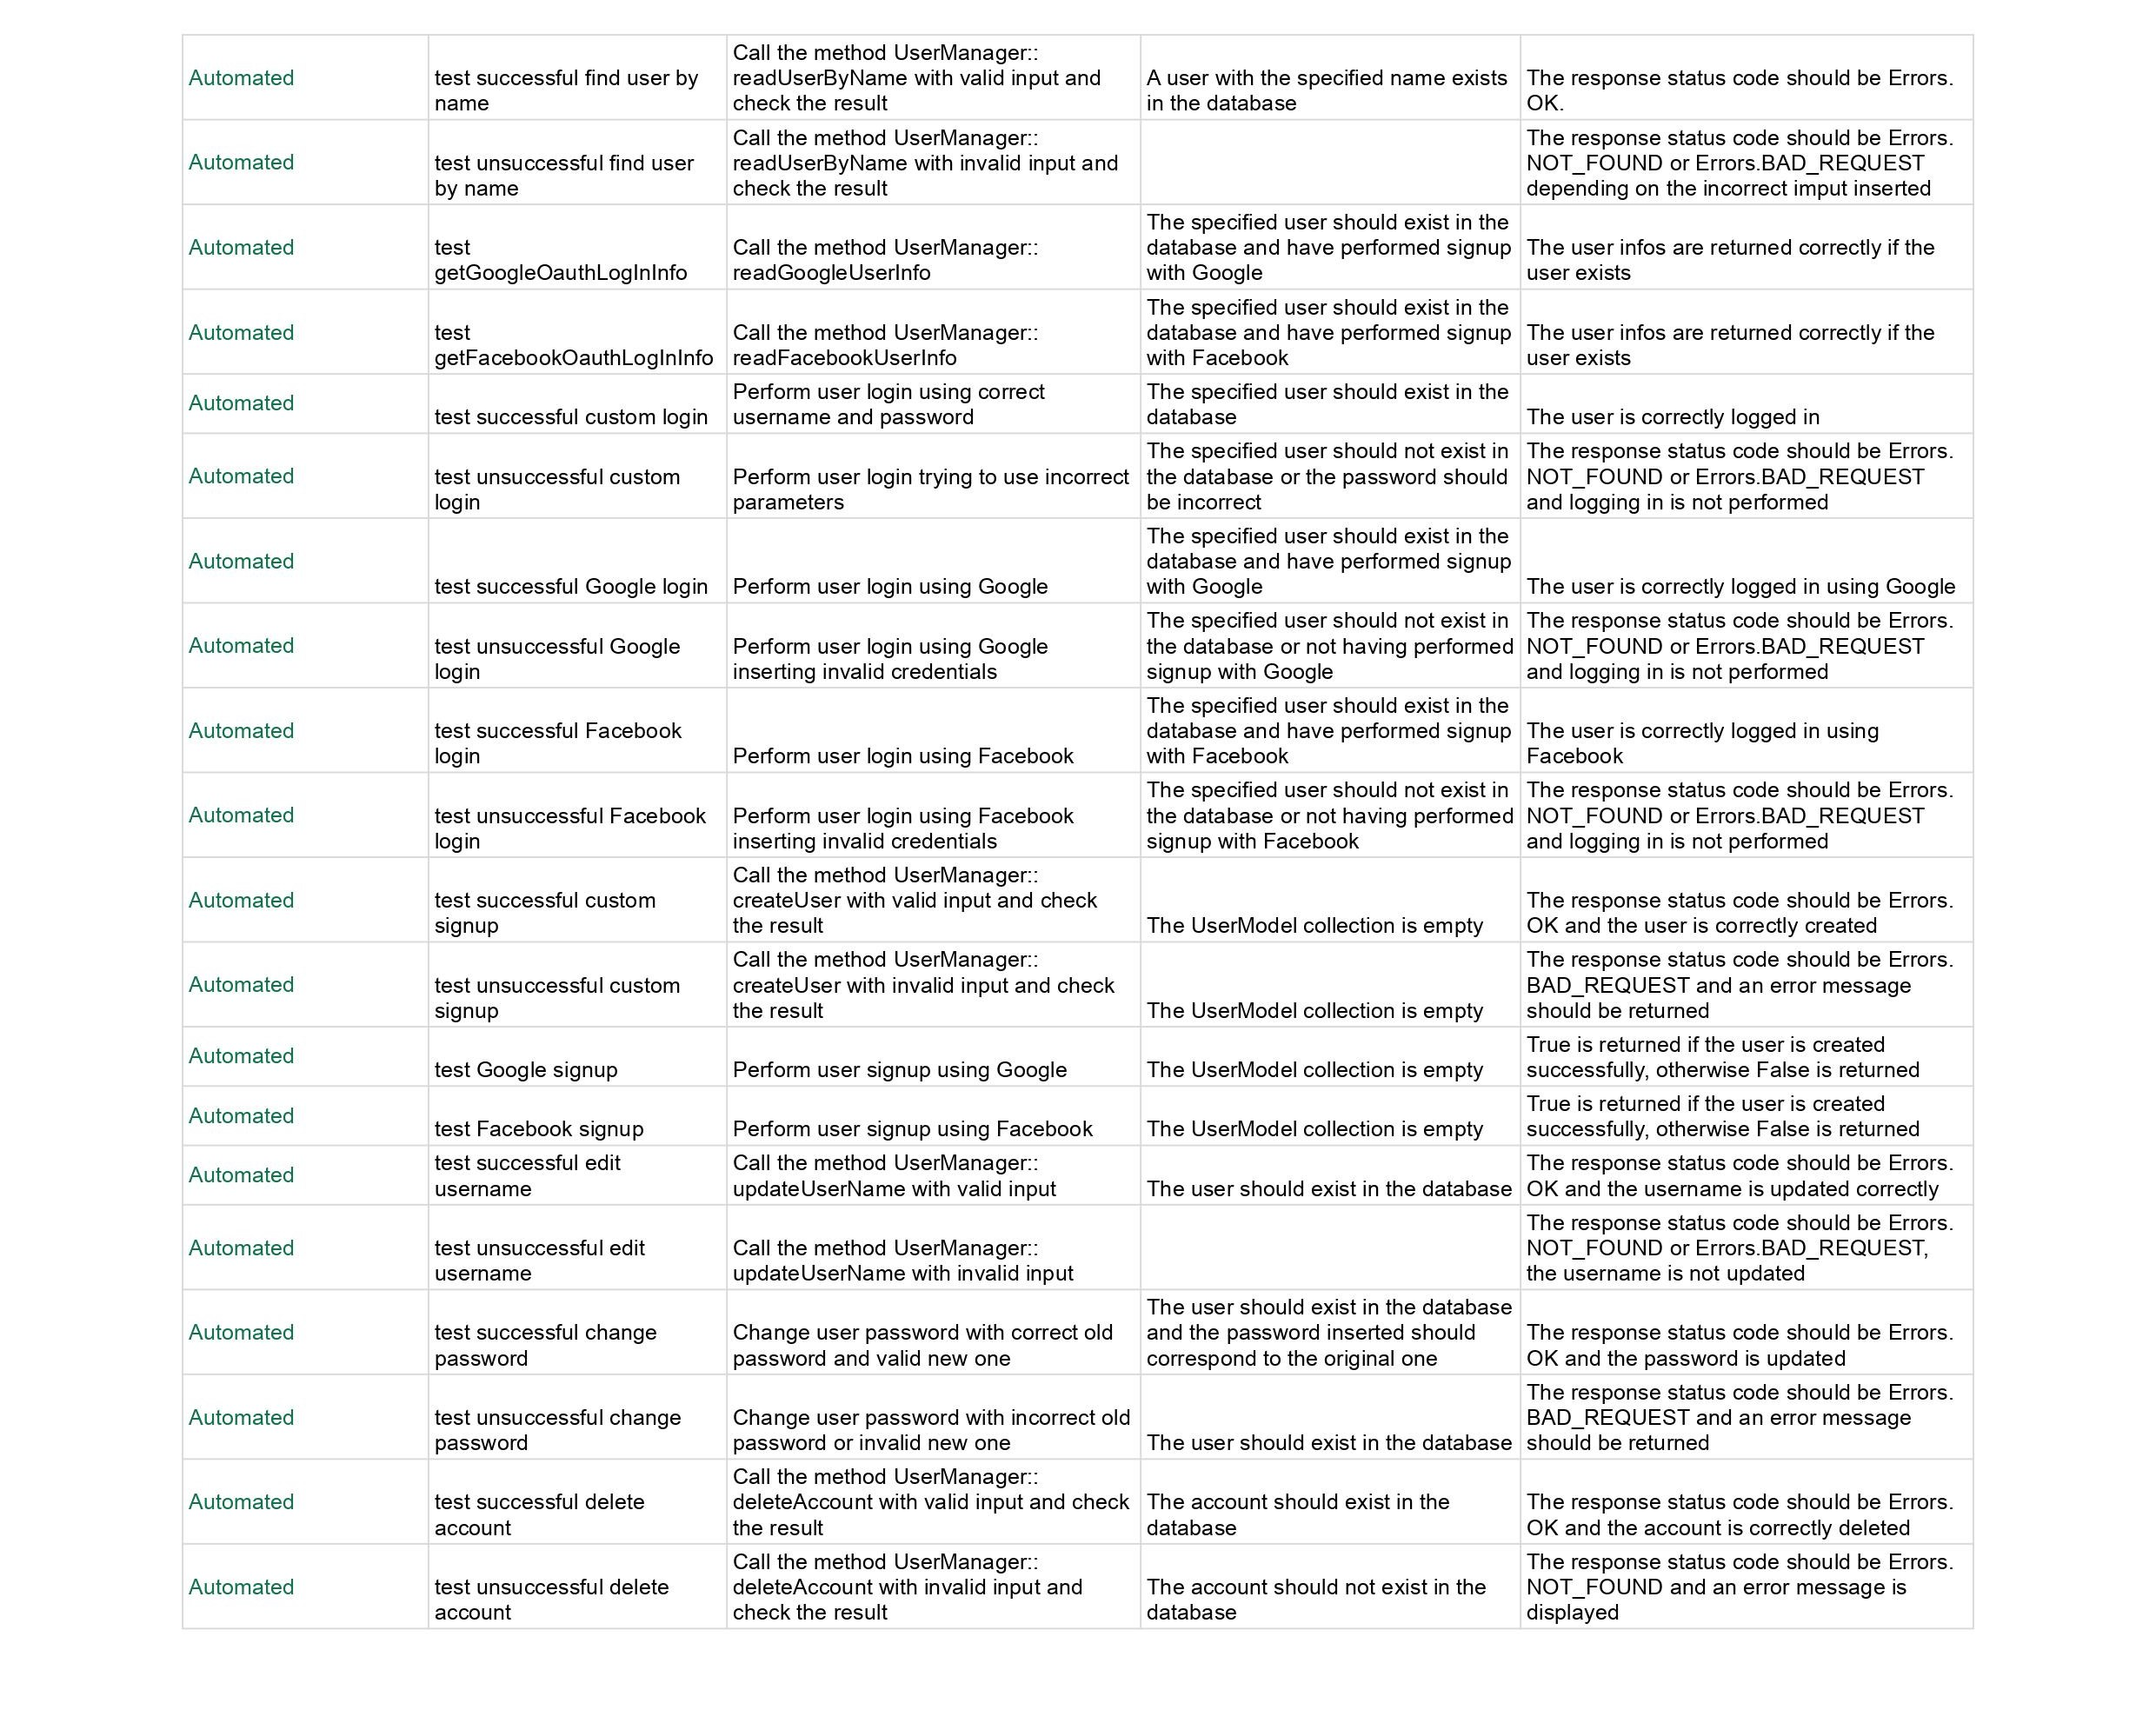
\includegraphics[width=0.95\textwidth]{images/Test_AccountManager.jpg}

\subsection*{Test DatabaseManager::UserManager}
This section is dedicated to the tests for the UserManager class, which is responsible for managing users in the database.
\newline
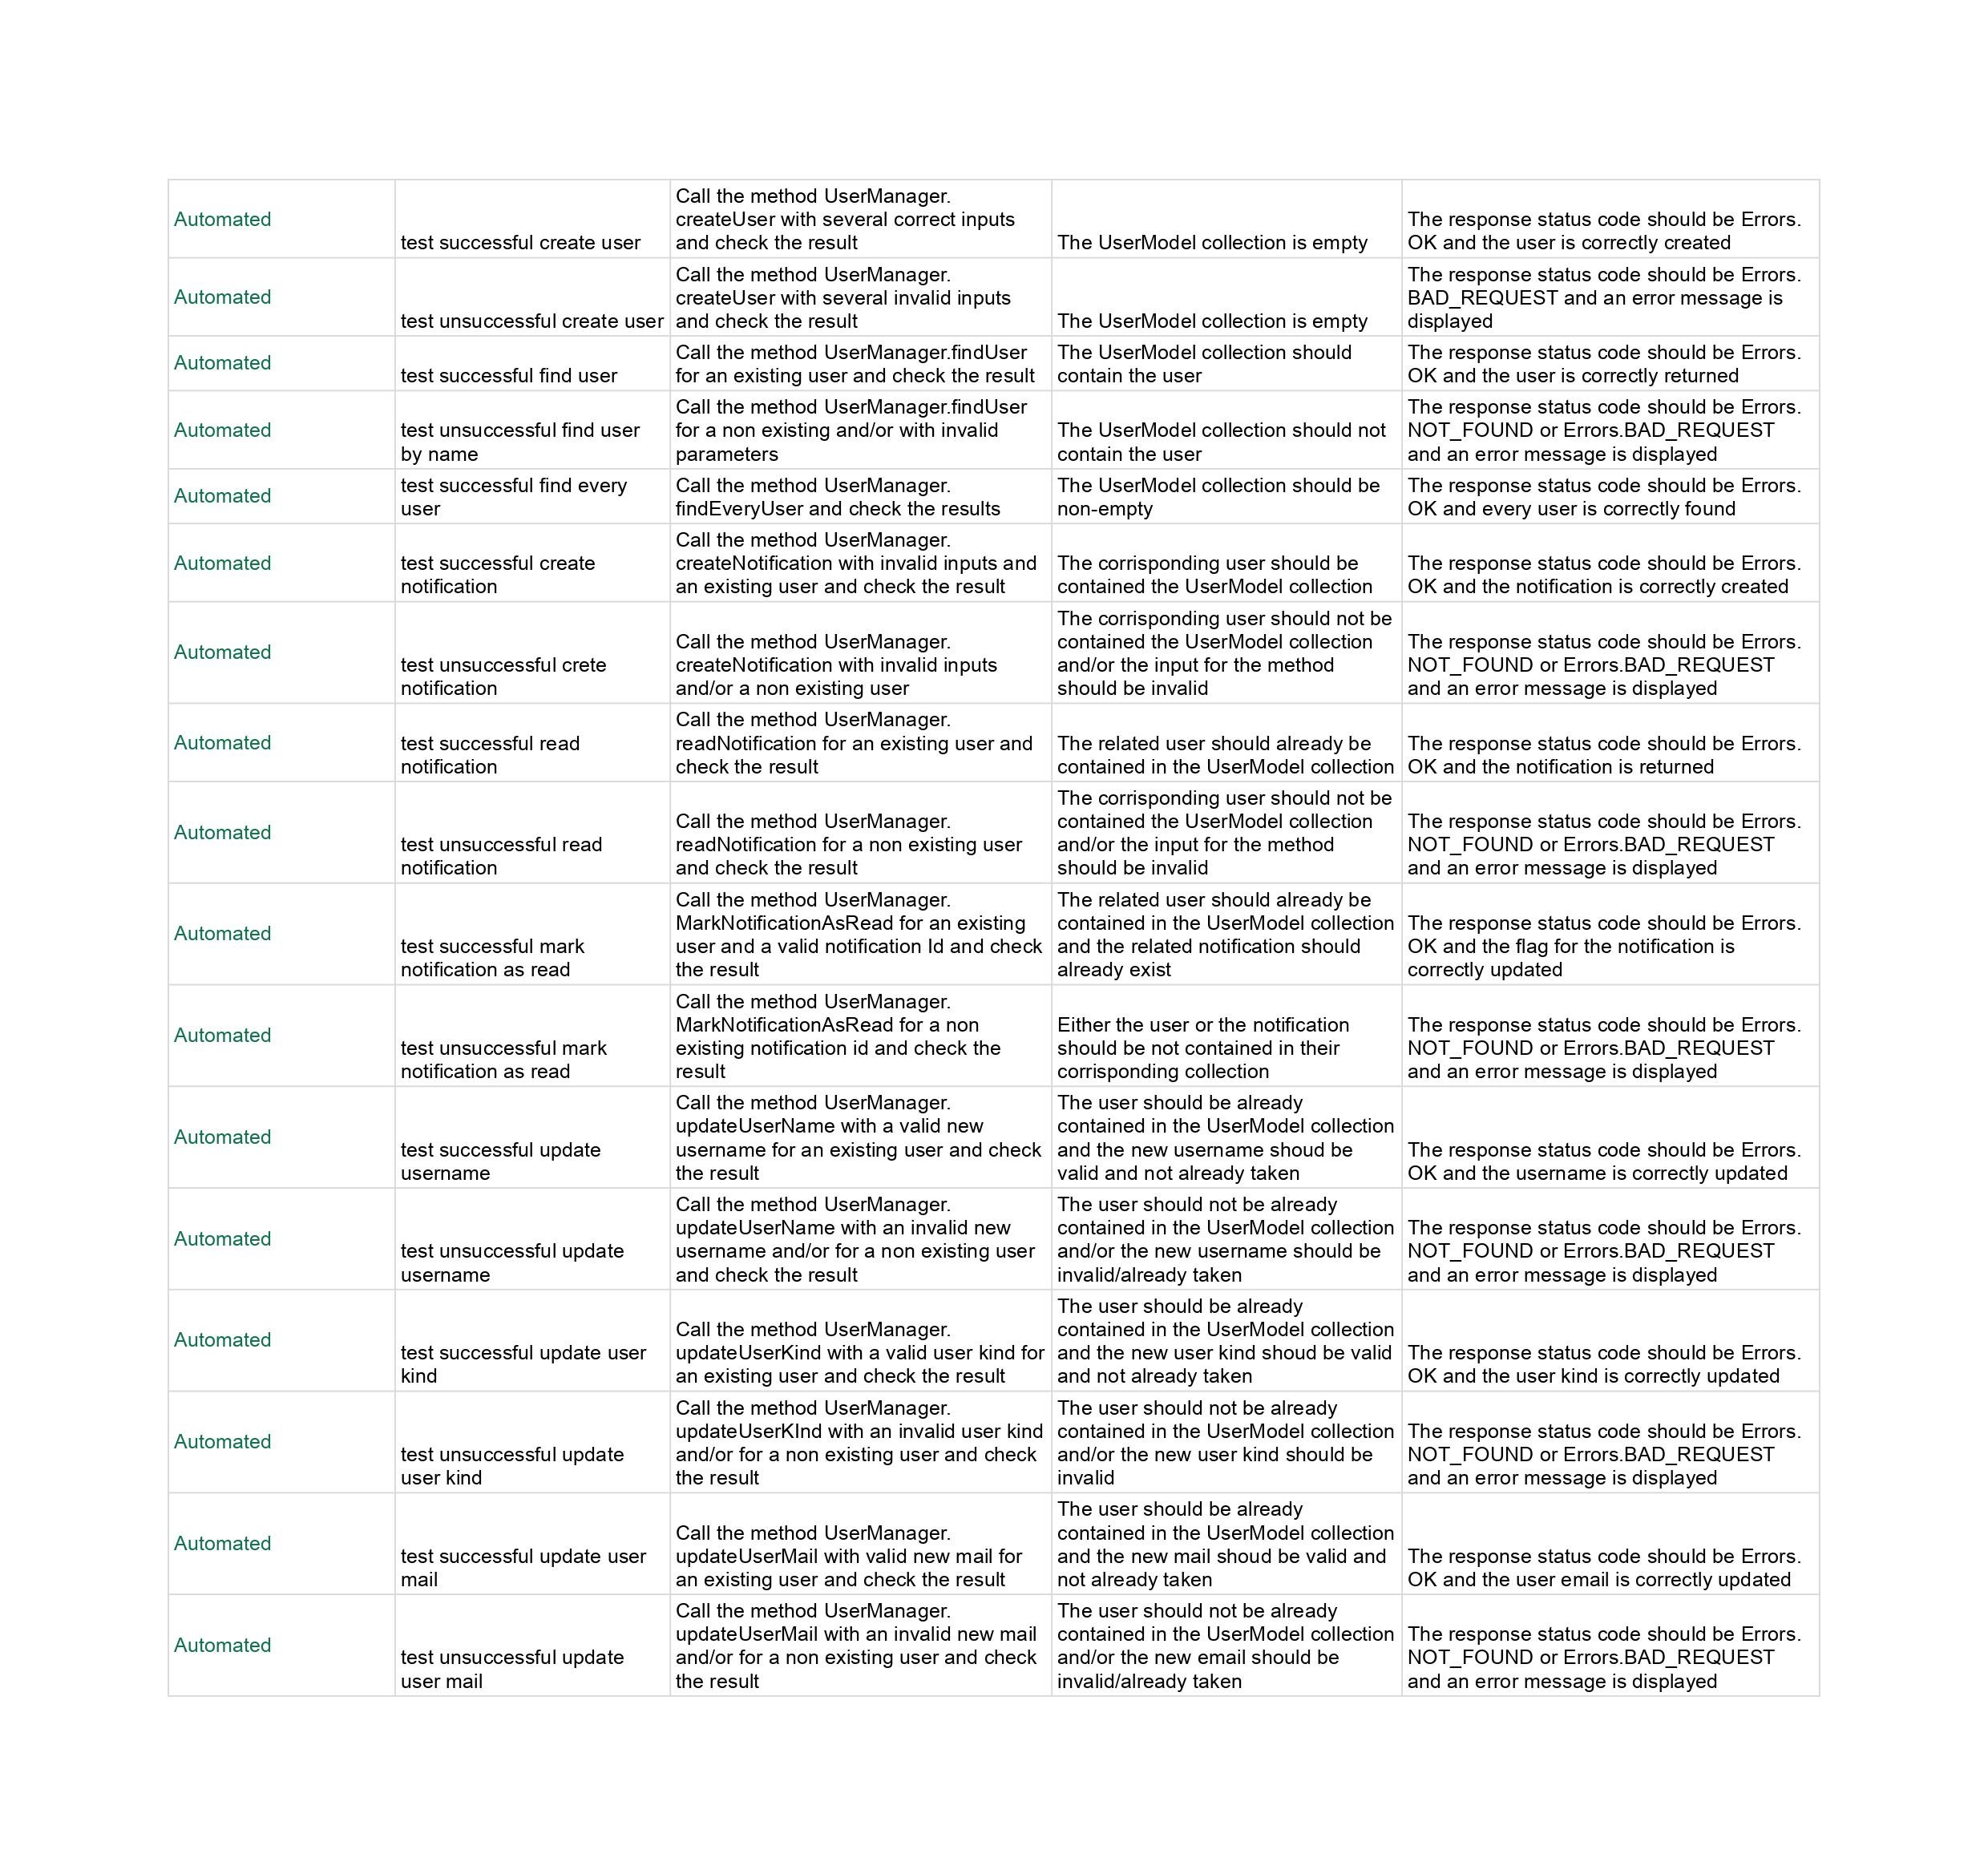
\includegraphics[width=0.95\textwidth]{images/Test_DatabaseManagerUserManager.jpg}

\subsection*{Test TaskManager}
This section includes automated tests for the TaskManager class, which is responsible for managing tasks in the database.
\newline
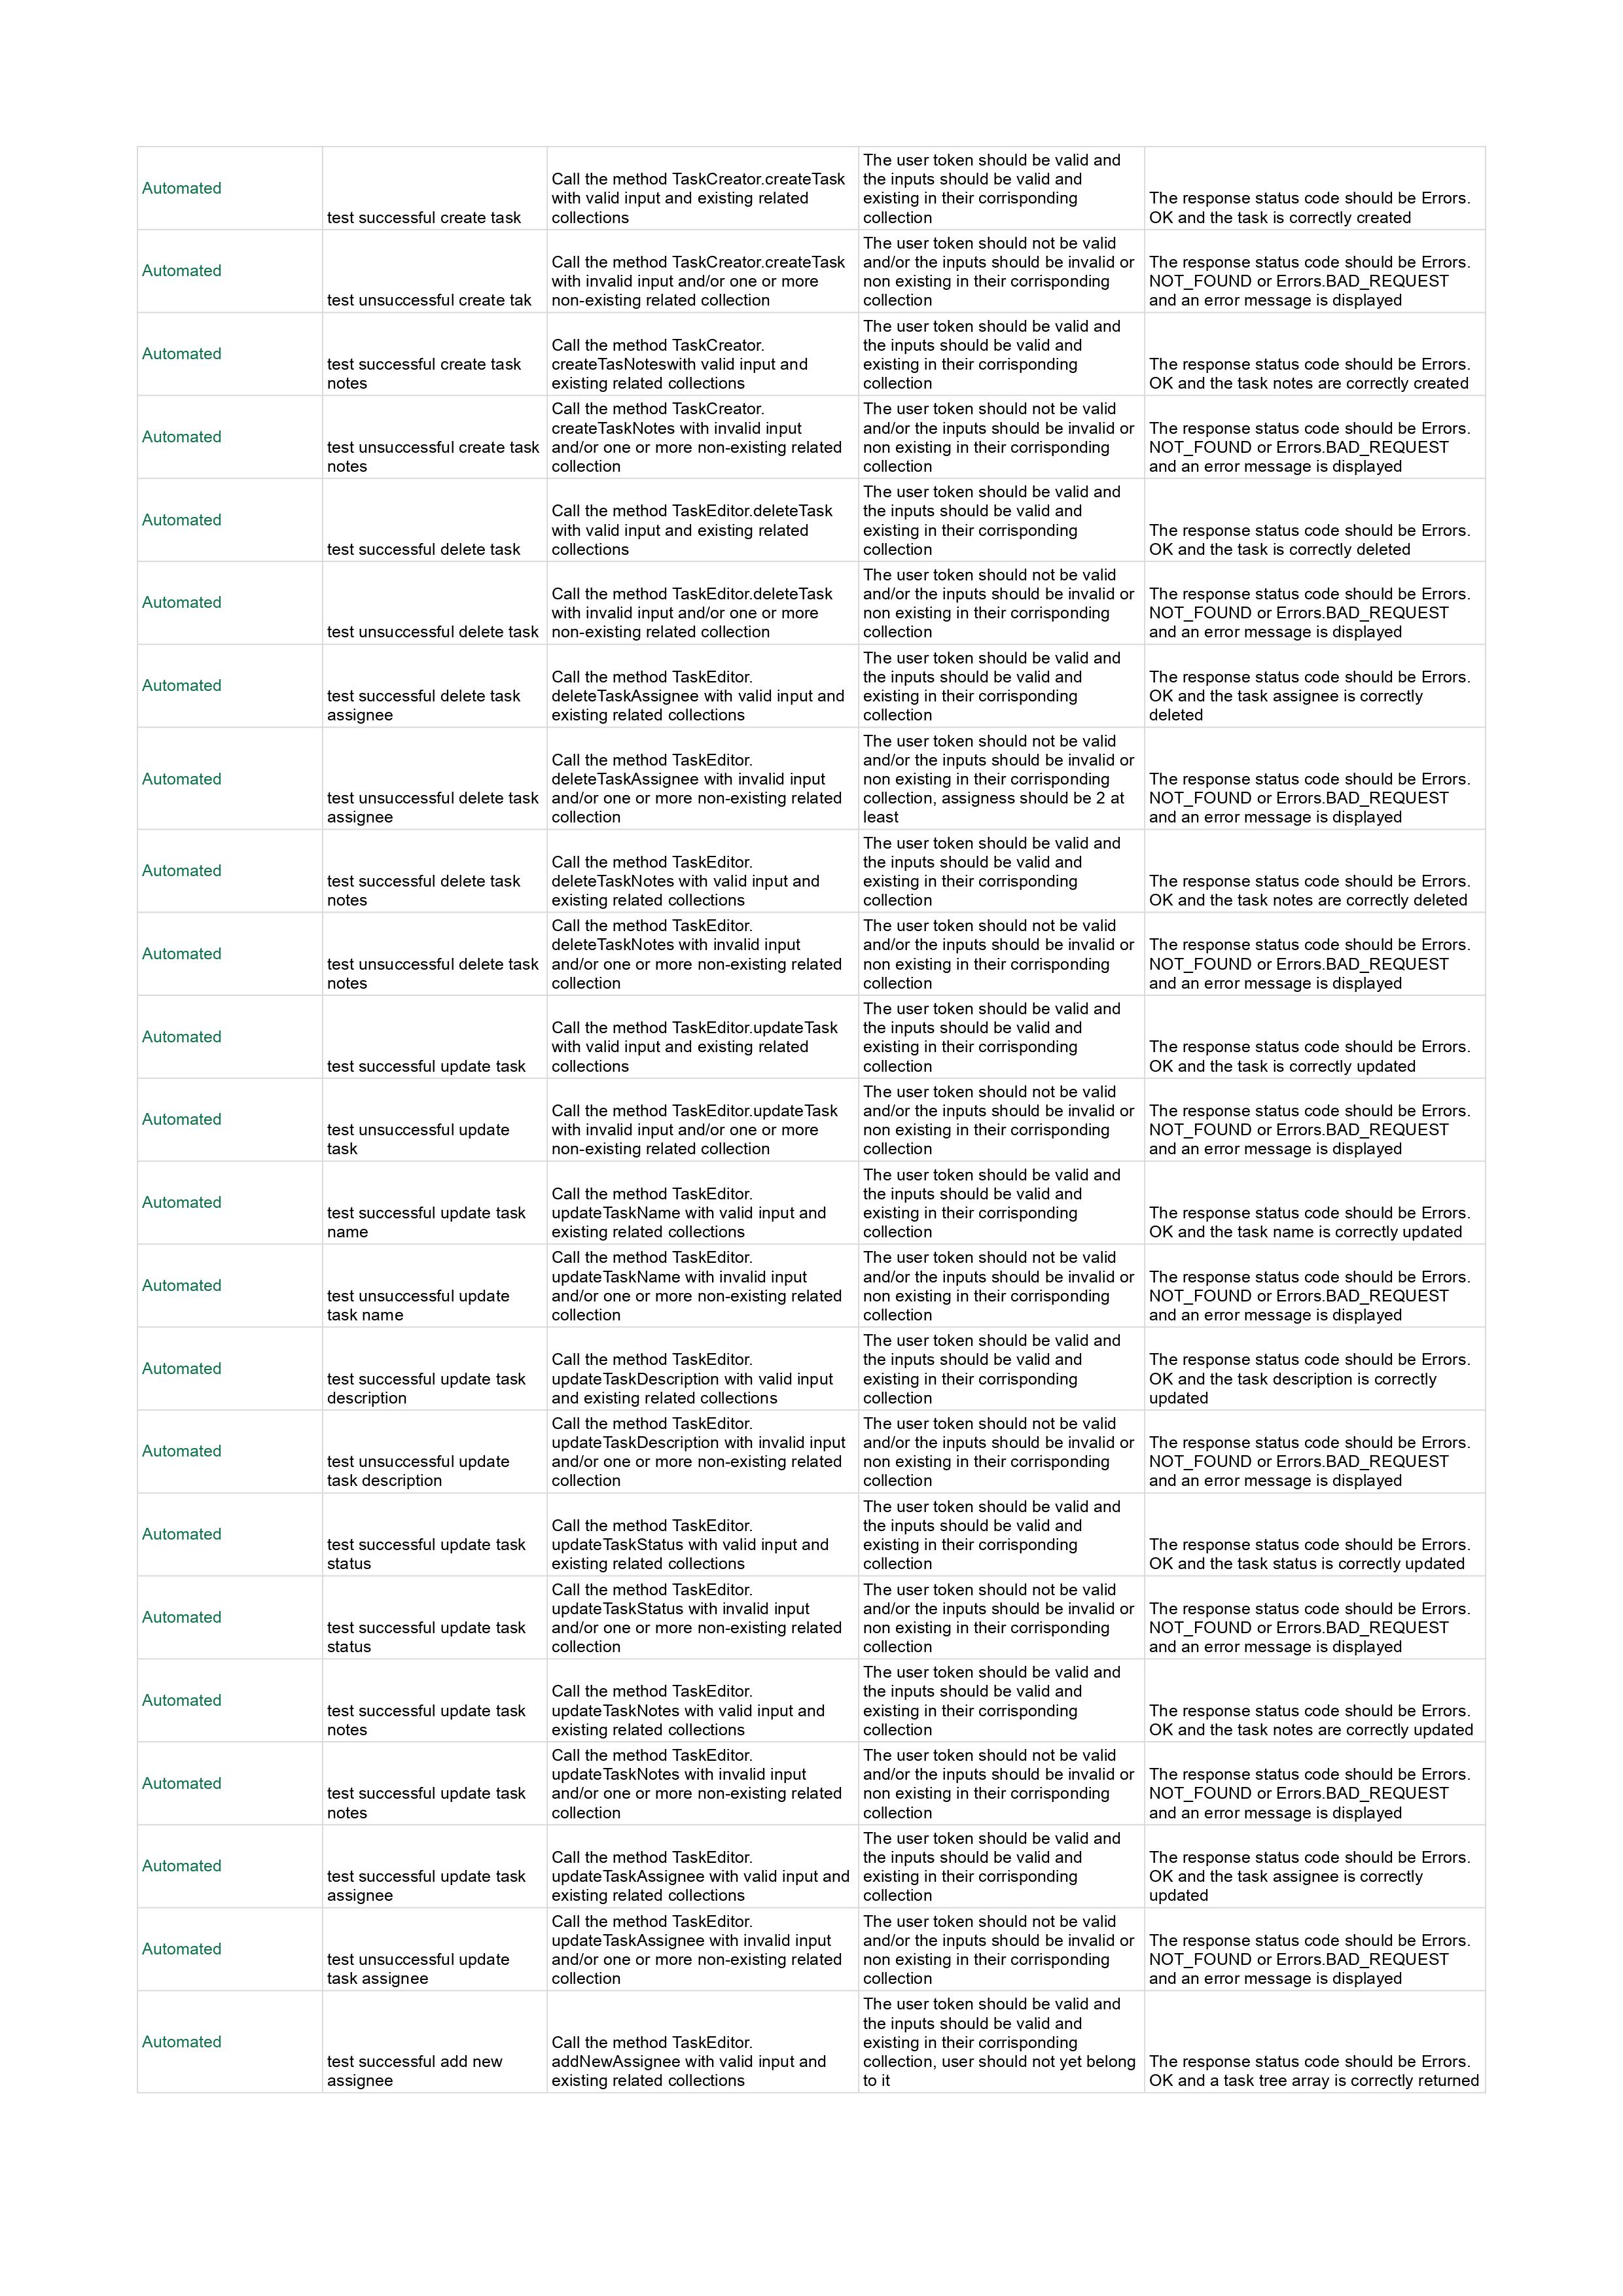
\includegraphics[width=0.95\textwidth]{images/Test_TaskManager-immagini-0.jpg}
\newline
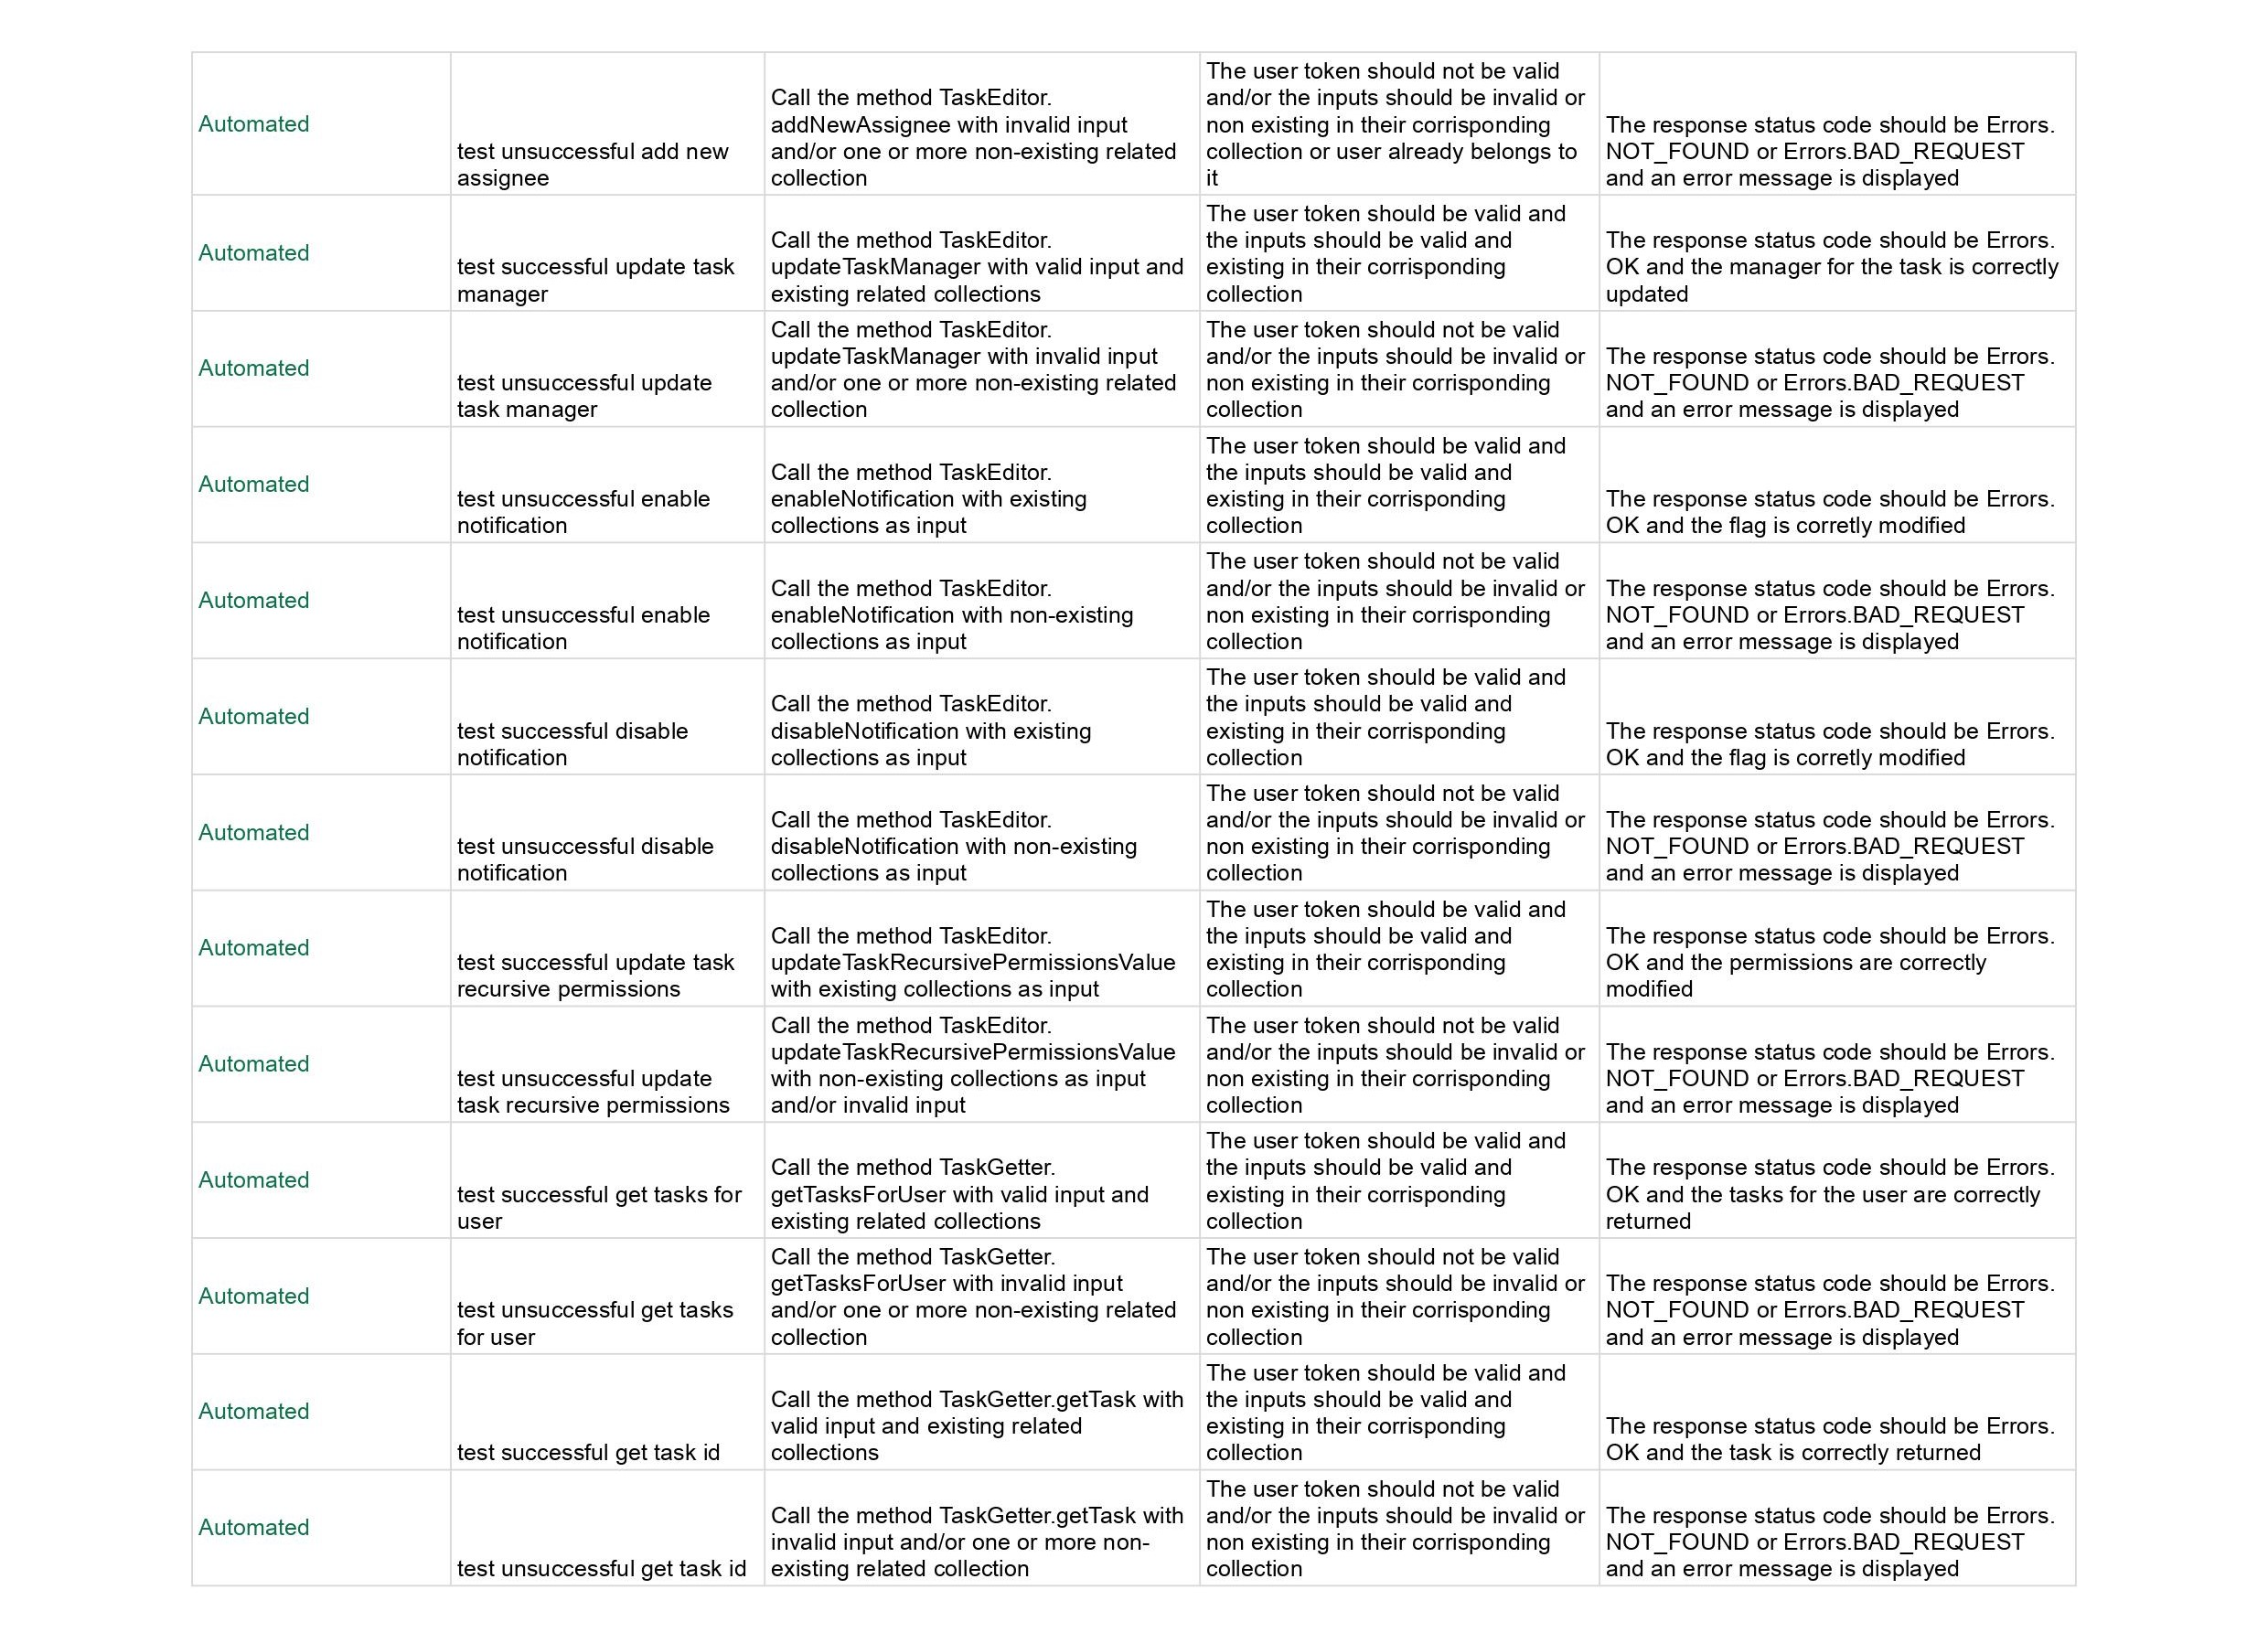
\includegraphics[width=0.95\textwidth]{images/Test_TaskManager-immagini-1.jpg}

\subsection*{Test Home Page}
This section includes manual tests for the home page.
\newline
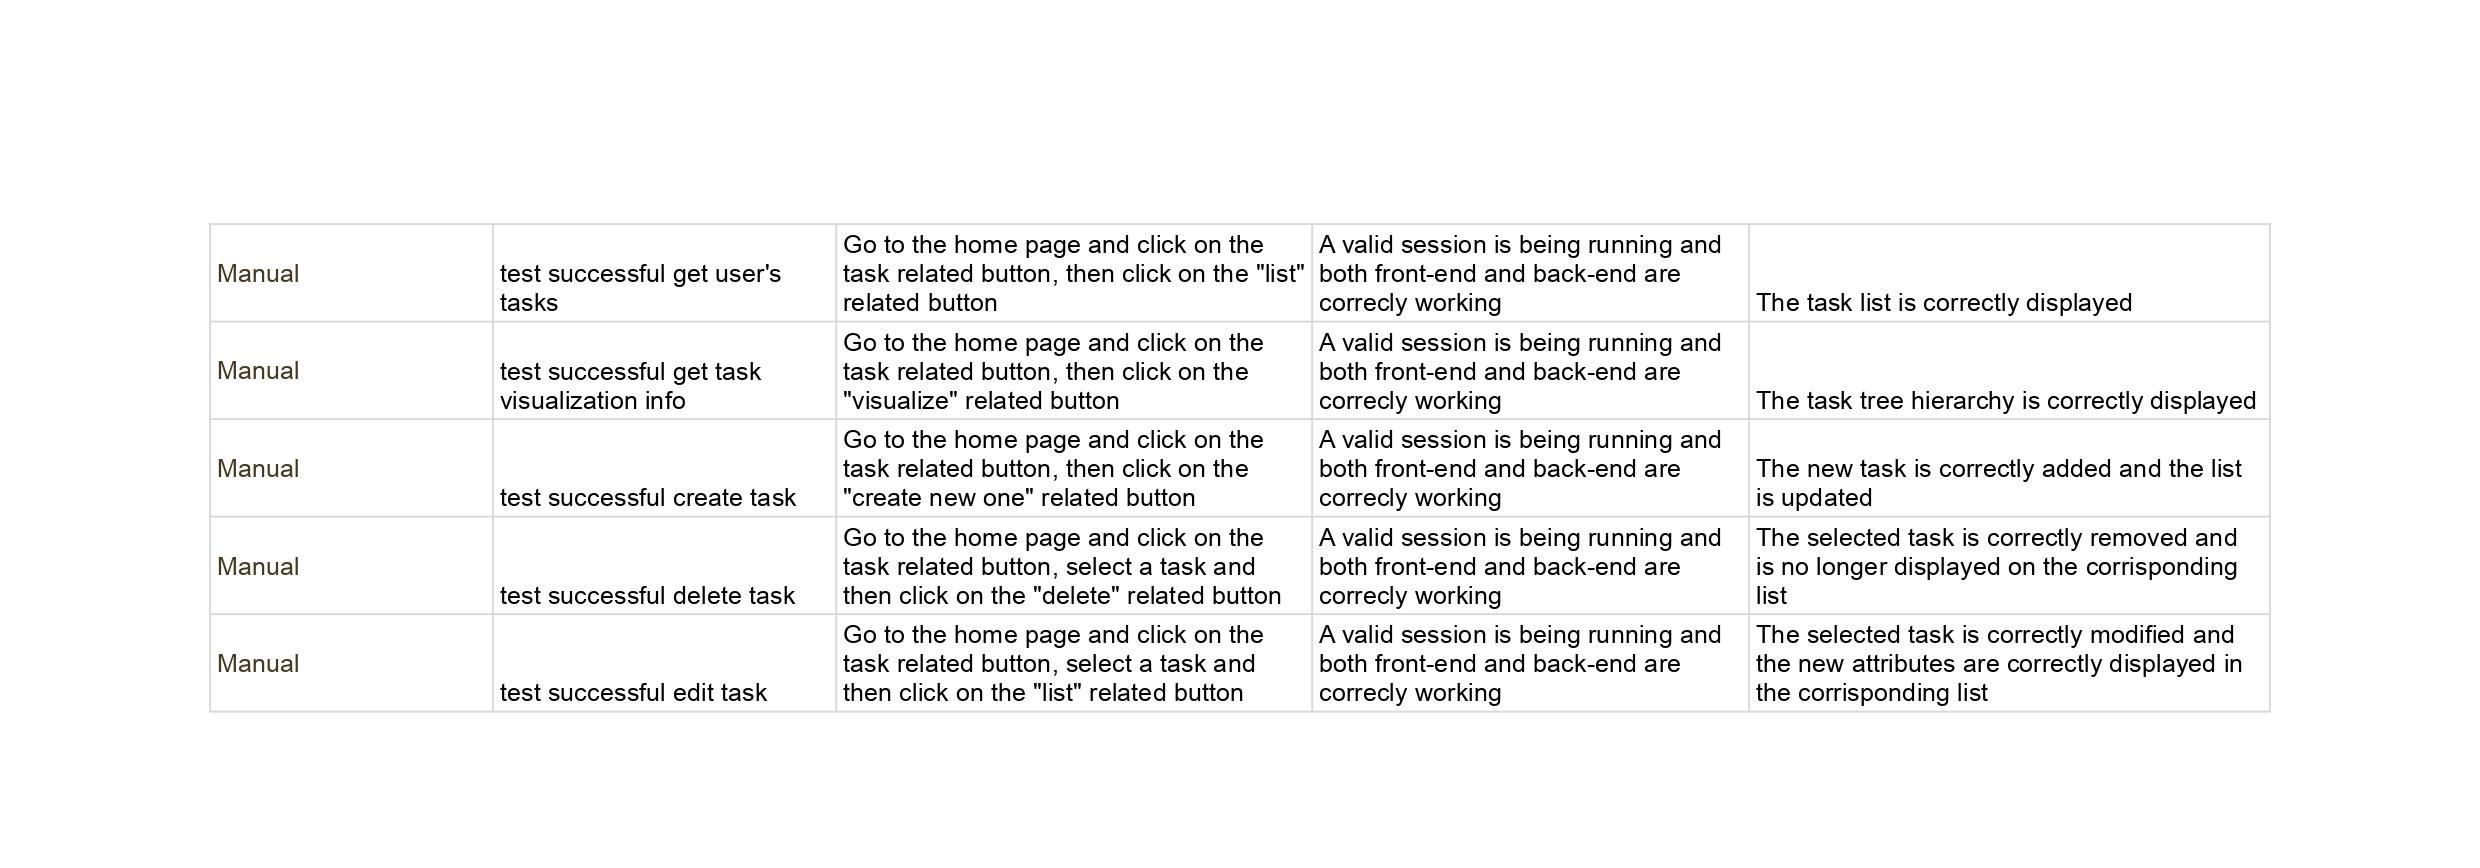
\includegraphics[width=0.95\textwidth]{images/Test_HomePage.jpg}

\subsection*{Test Notification View}
This section includes manual tests for the notification view.
\newline
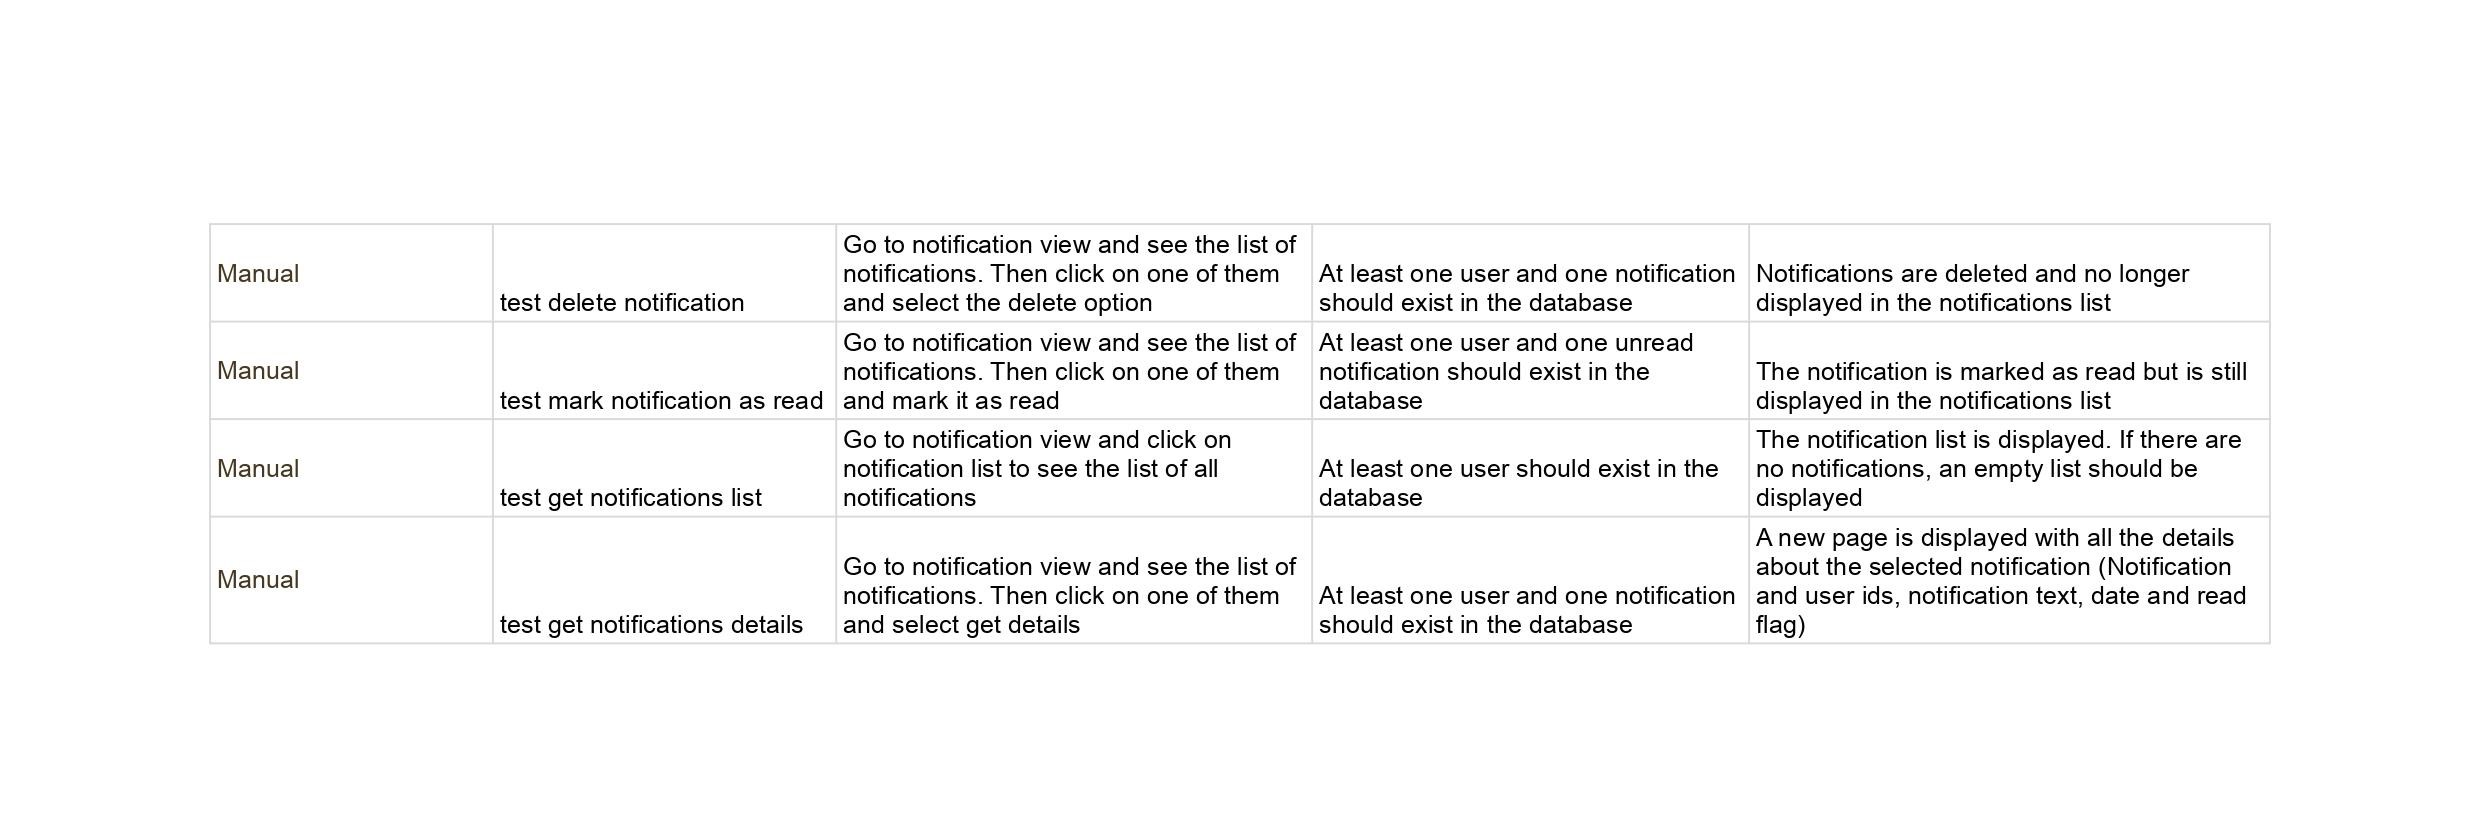
\includegraphics[width=0.95\textwidth]{images/Test_NotificationView.jpg}

\subsection*{Test Sign In and Sign Up Pages}
This section includes manual tests for the sign in and sign up pages.
\newline
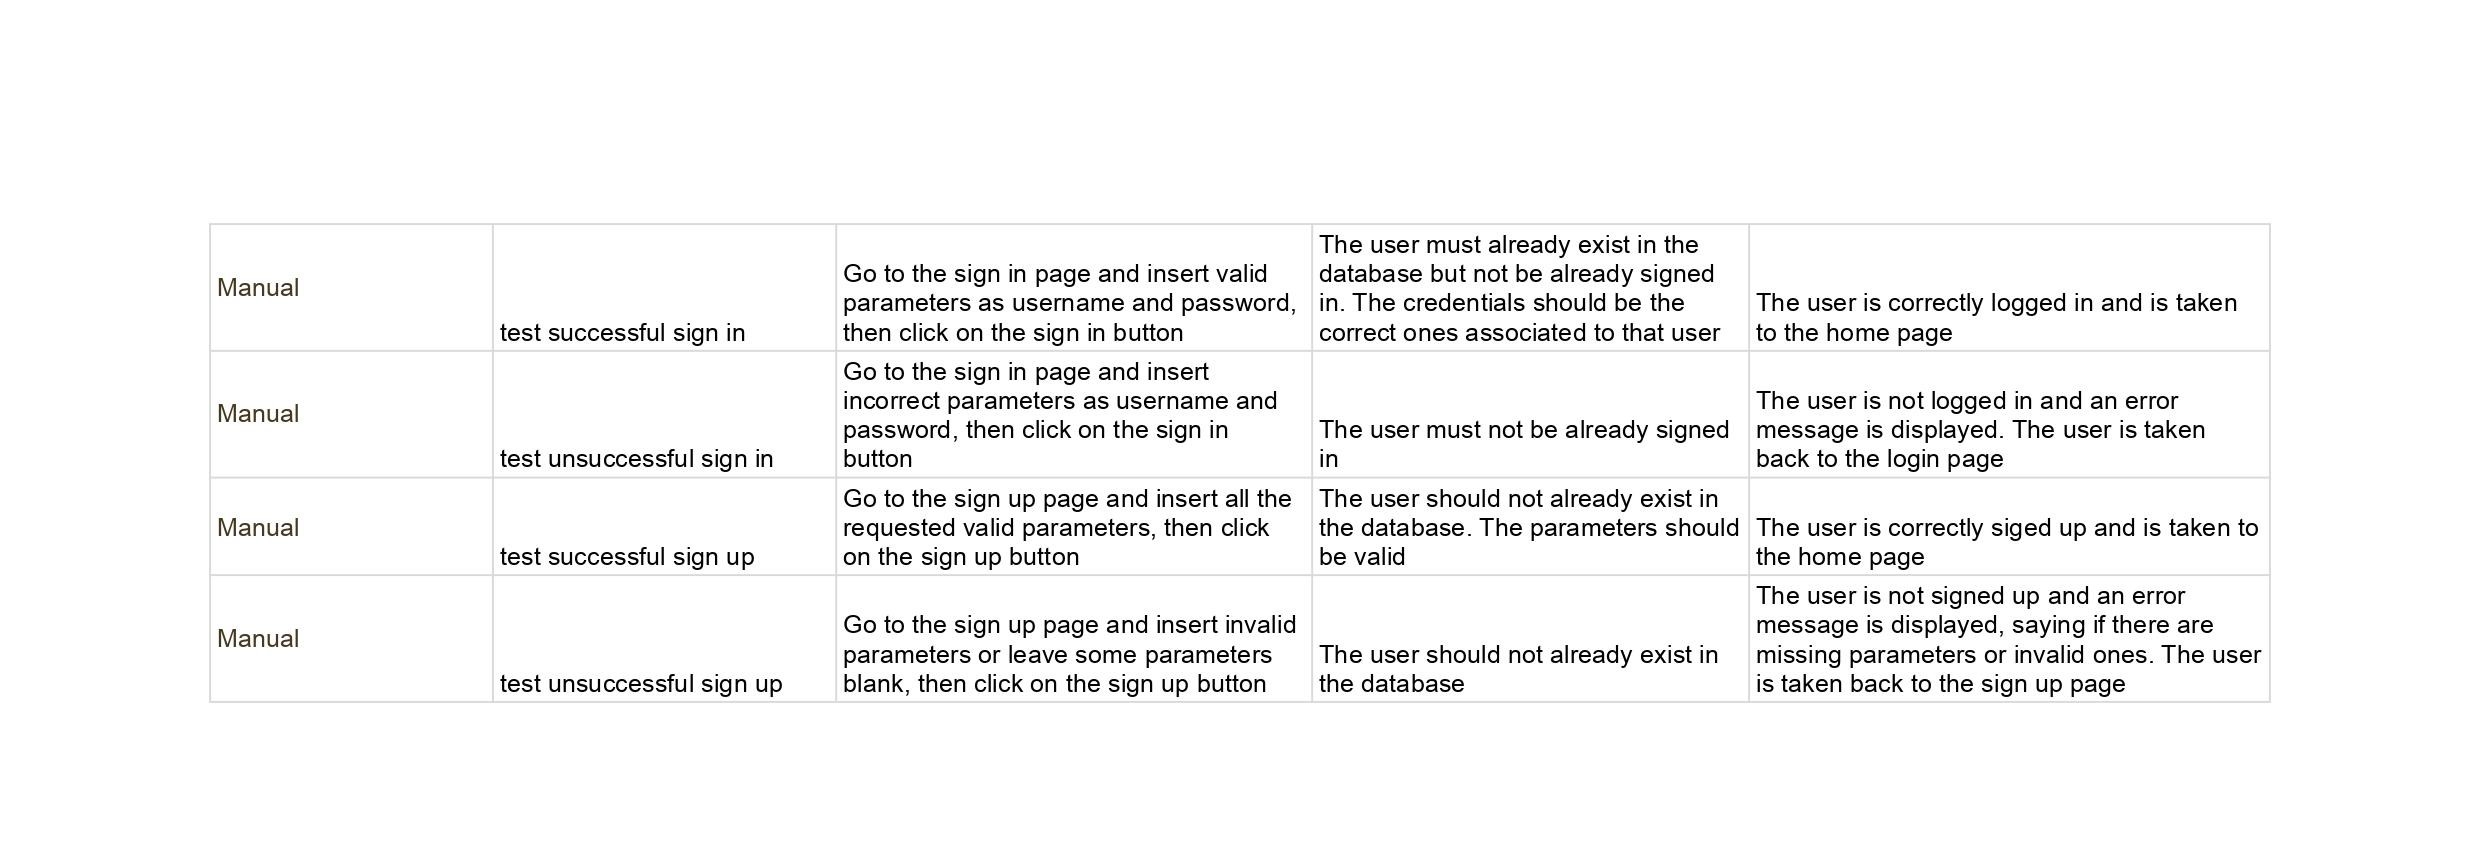
\includegraphics[width=0.95\textwidth]{images/Test_SignInSignUpPage.jpg}

\subsection*{Test Edit Profile Page}
This section includes manual tests for the edit profile page.
\newline
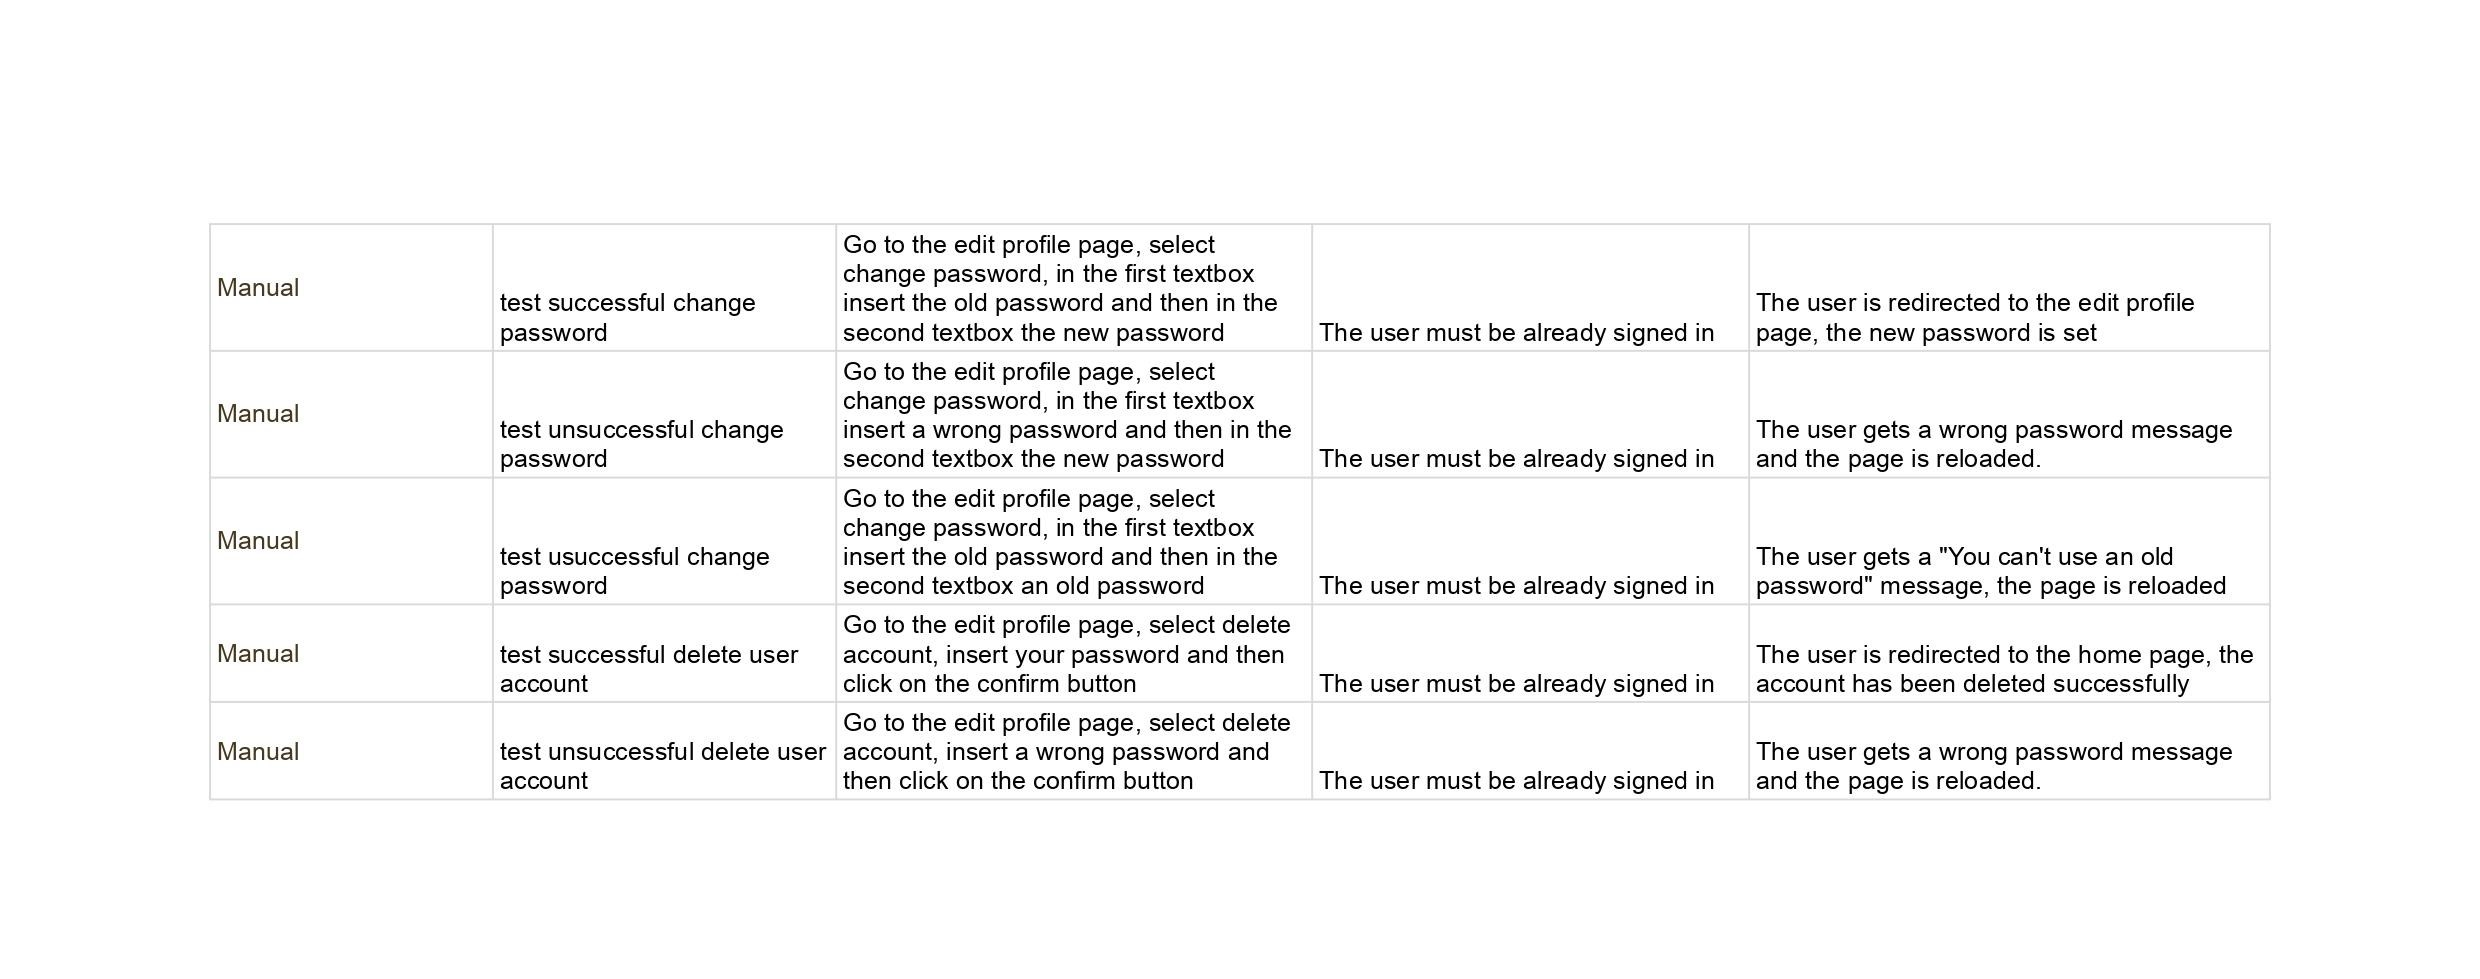
\includegraphics[width=0.95\textwidth]{images/Test_EditProfile.jpg}

\subsection*{Test Organization View Page}
This section includes manual tests for the organization view page.
\newline
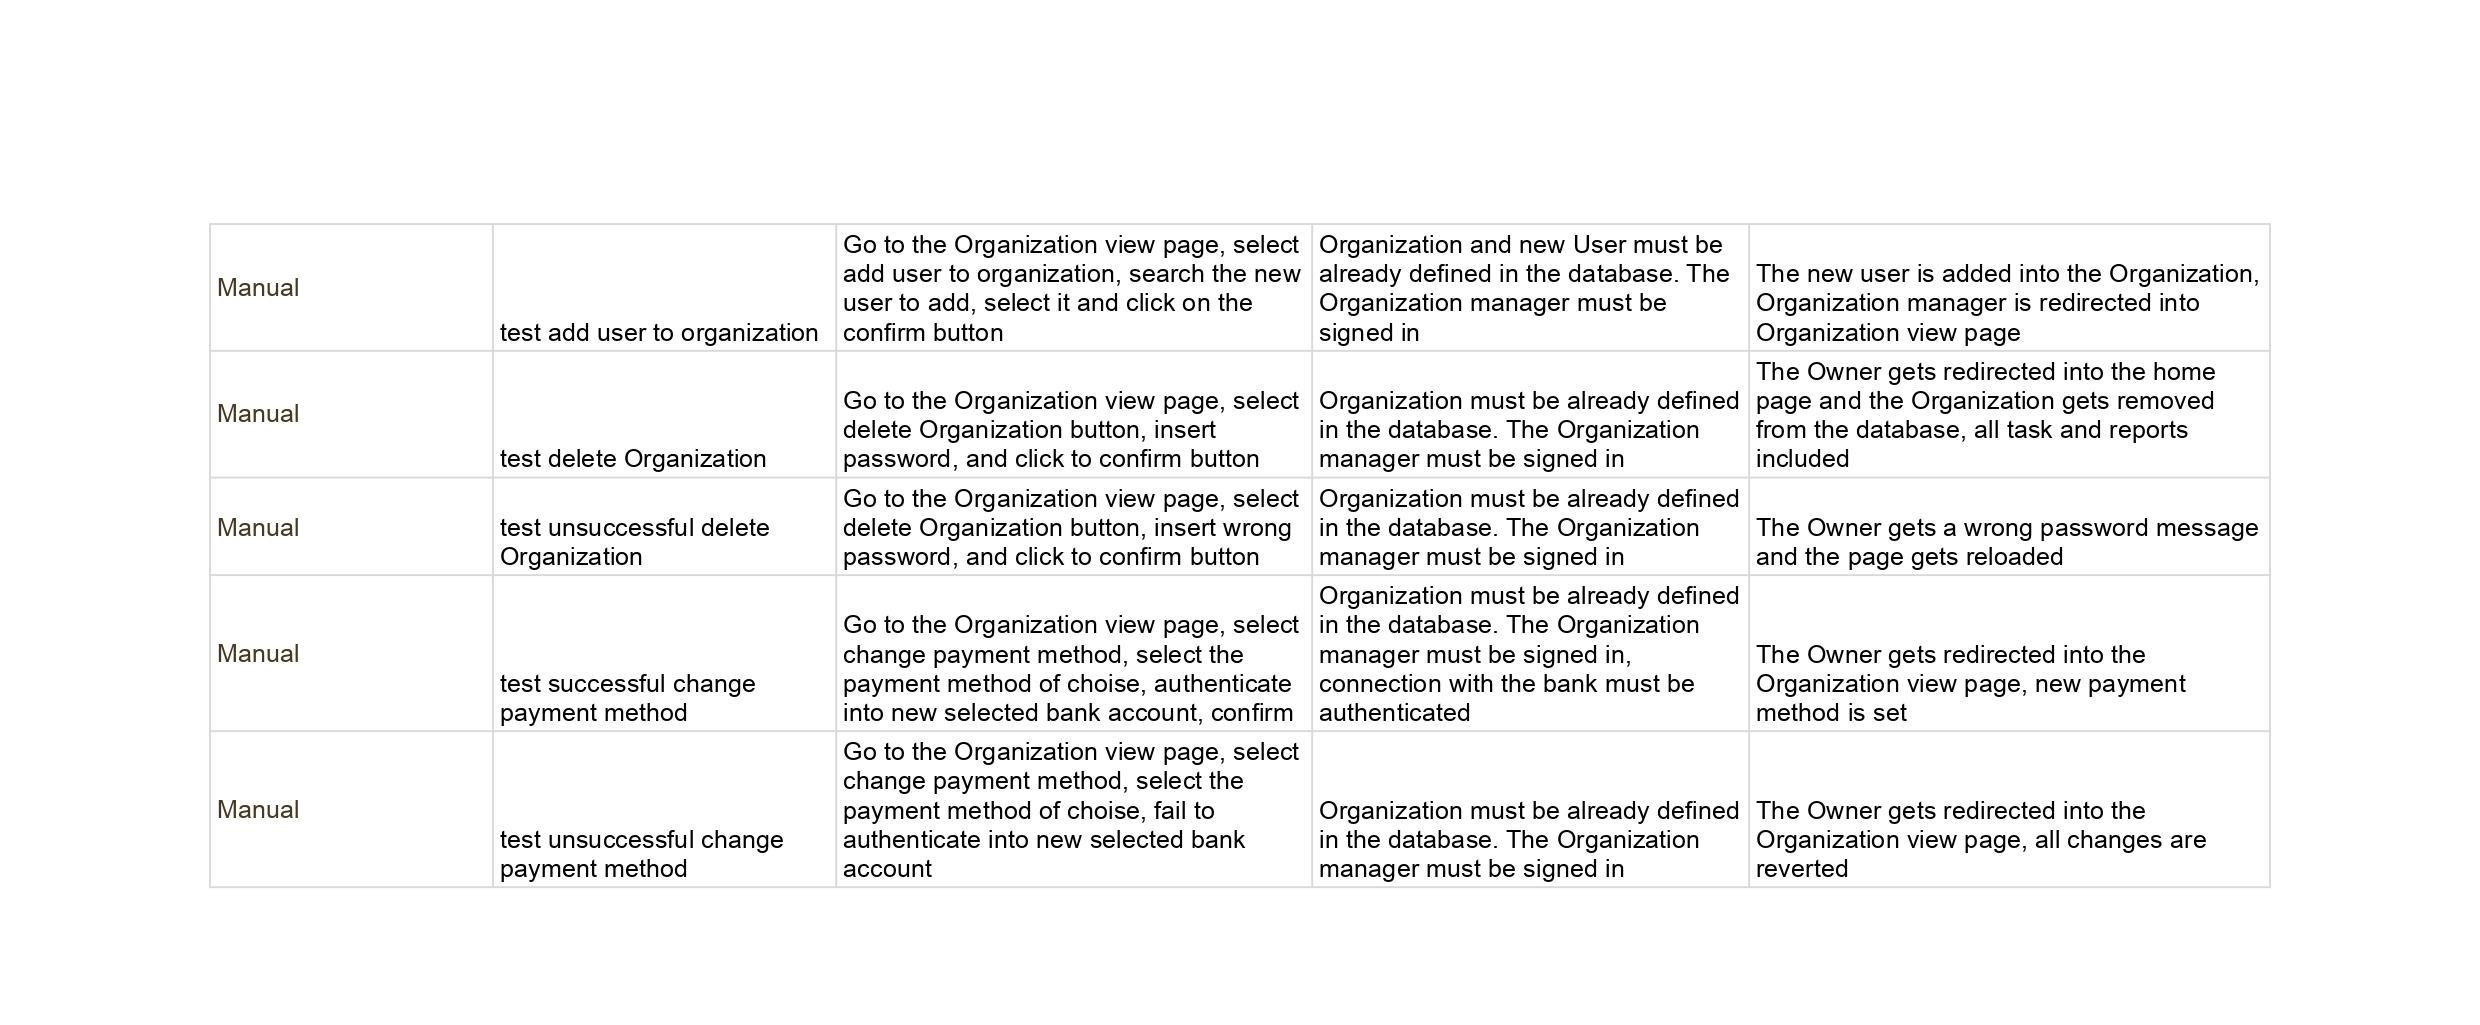
\includegraphics[width=0.95\textwidth]{images/Test_OrganizationView.jpg}

\section{Git Strategy}

Among the several git strategies available and commonly used, we have chosen \textbf{GitHub Flow}. We selected this strategy because it is \textit{one of the simplest} and is particularly suitable for \underline{small teams} like ours. GitHub Flow's straightforward approach, centered around a single branch with short-lived feature branches, allows us to maintain a \textbf{clean and manageable codebase}. This strategy also facilitates \textit{continuous integration and delivery}, making it easier to track progress and integrate changes seamlessly.



\section{Sprint 1}

\subsection{Backlog}
\includegraphics[width=0.95\textwidth]{images/sprint_backlog.jpg}

\subsection{Review and Retrospective}
\subsubsection{Retrospective}
Overall, the sprint was successful, as we managed to complete all the tasks on time.

We experienced some minor slowdowns due to our unfamiliarity with \textit{JavaScript} and \textit{MongoDB}, but we ultimately overcame these challenges. This sprint has been a valuable learning experience, highlighting areas where we can improve our technical skills.

In terms of task estimation, our decision to adopt a \textbf{conservative approach} proved to be beneficial. The higher estimates allowed us to allocate sufficient time to each task, reducing stress and enabling us to handle unforeseen issues effectively.

Team coordination was commendable, though there is room for improvement. The \underline{meticulous division of labor} contributed significantly to our success. Each member had a clear understanding of their responsibilities, which facilitated smoother collaboration and minimized overlapping efforts. However, we need to refine our task distribution further to optimize efficiency.

One notable area for improvement is our handling of \textbf{code integration}. Merging diverging branches proved to be time-consuming and occasionally disrupted our workflow. To address this, we should implement more frequent integration practices and establish clearer guidelines for branch management. This will help us avoid the pitfalls of merging conflicts and enhance our overall productivity.

Looking ahead to the upcoming sprint, we should focus on better organizing the workload across the team. By distributing tasks more evenly and ensuring that everyone is aligned with our coding standards and best practices, we can mitigate potential bottlenecks and maintain a steady progress rate.

Additionally, we should continue to invest time in learning and mastering the technologies we are using. This will not only boost our efficiency but also increase the quality of our product.

In conclusion, while this sprint has been a success, it also highlighted several areas for potential growth. By addressing these issues and building on our strengths, we can look forward to an even more productive standard for out team as a whole.

\subsubsection{Review}

Due to the subset of the chosen tasks we did't have too much to show to the ``Product Owner'' at the end of the sprint.
We shown the automatic deployment of the backend on render, and the frontend on GitHub Pages. We also shown the
automated tests to the backend functionalities.
Overall, the product Owner was satisfied with the results of the sprint, and didn't ask us to change anything.

\subsection{Burn-down Chart}
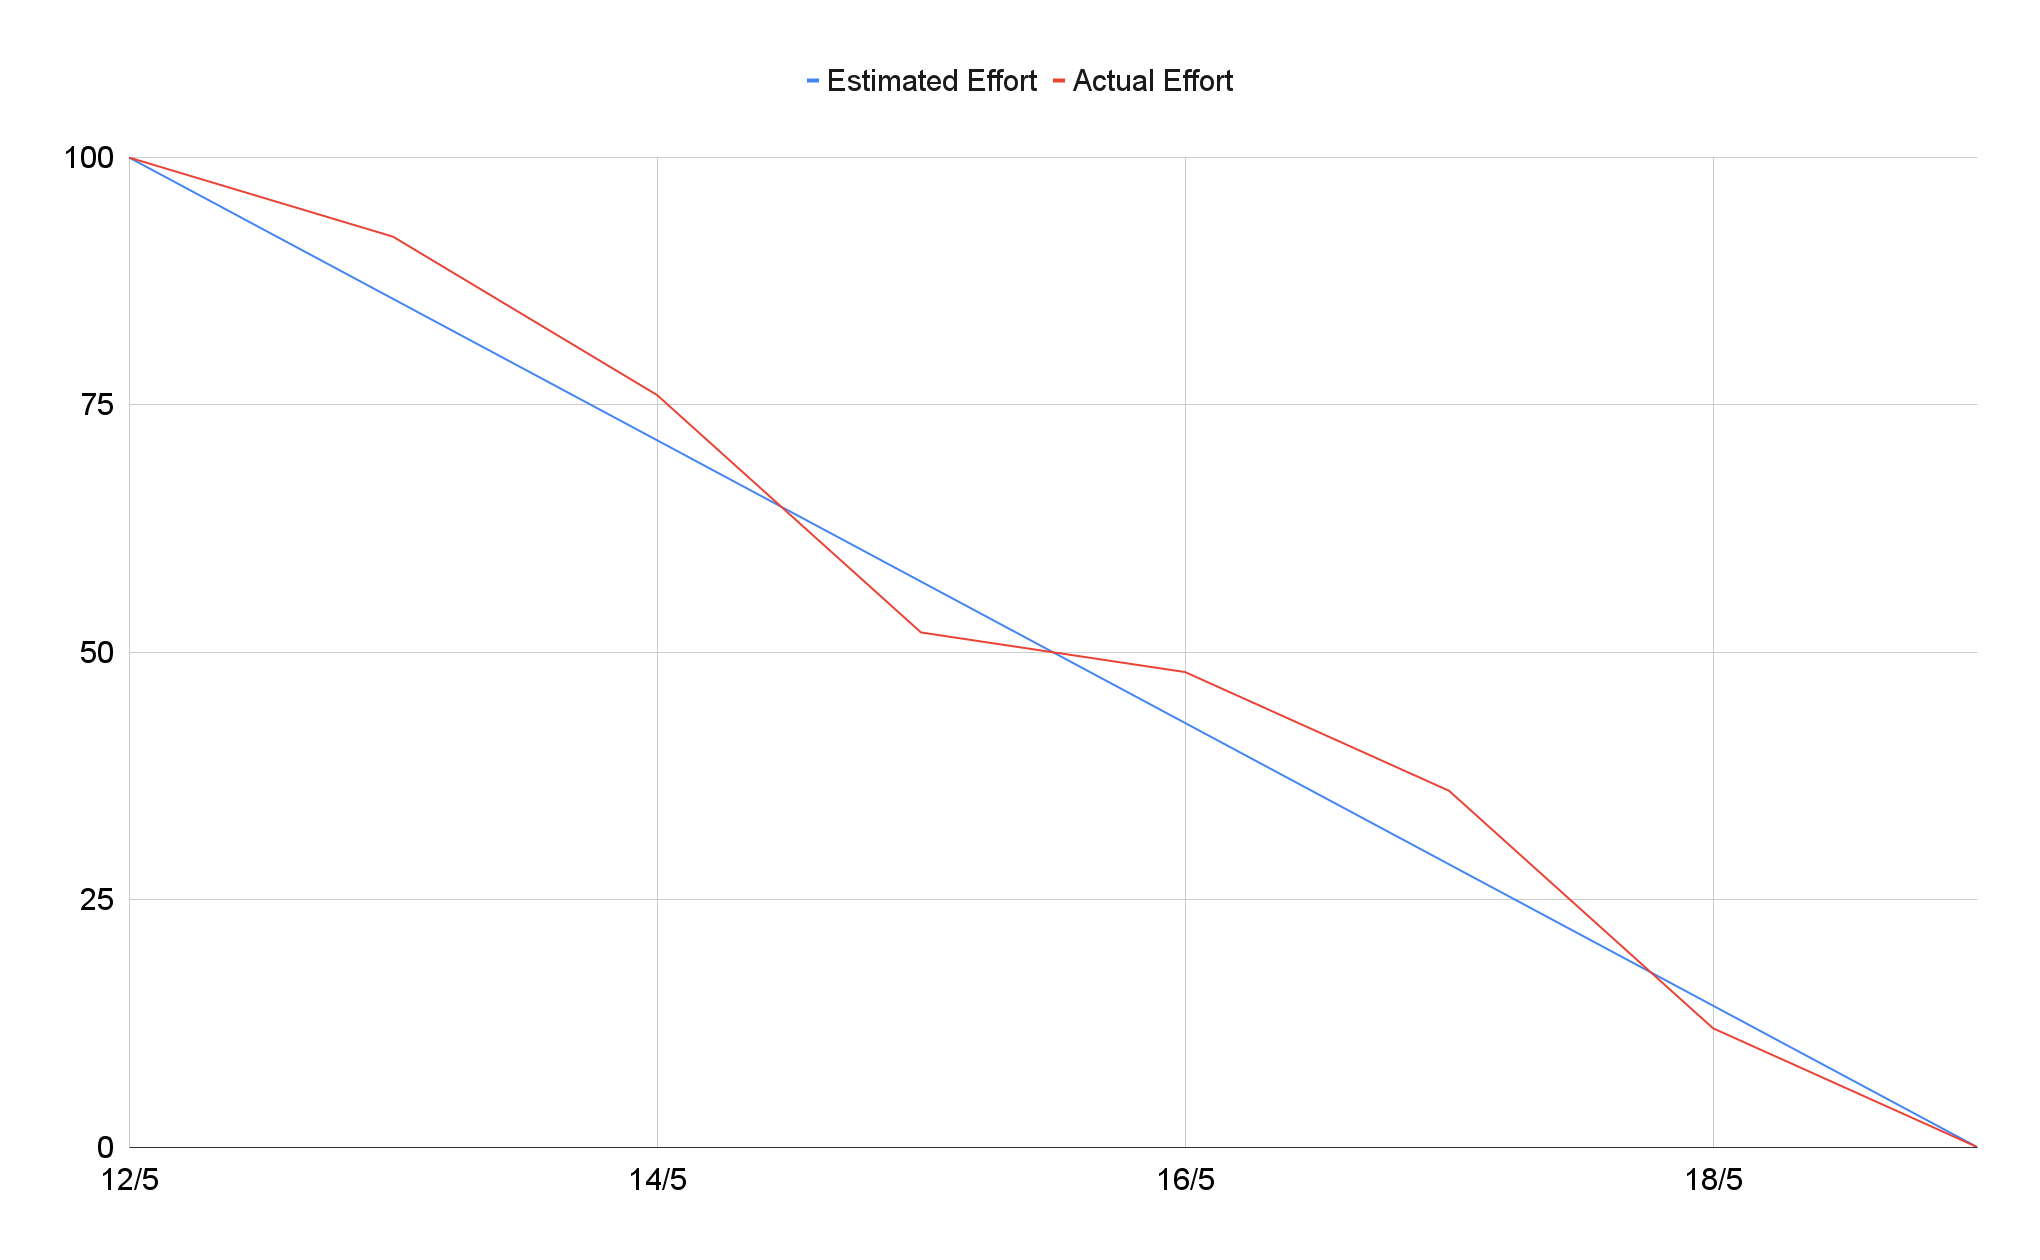
\includegraphics[width=0.95\textwidth]{images/burndown_chart.png}

\section{Sprint 2}

\subsection{Backlog}
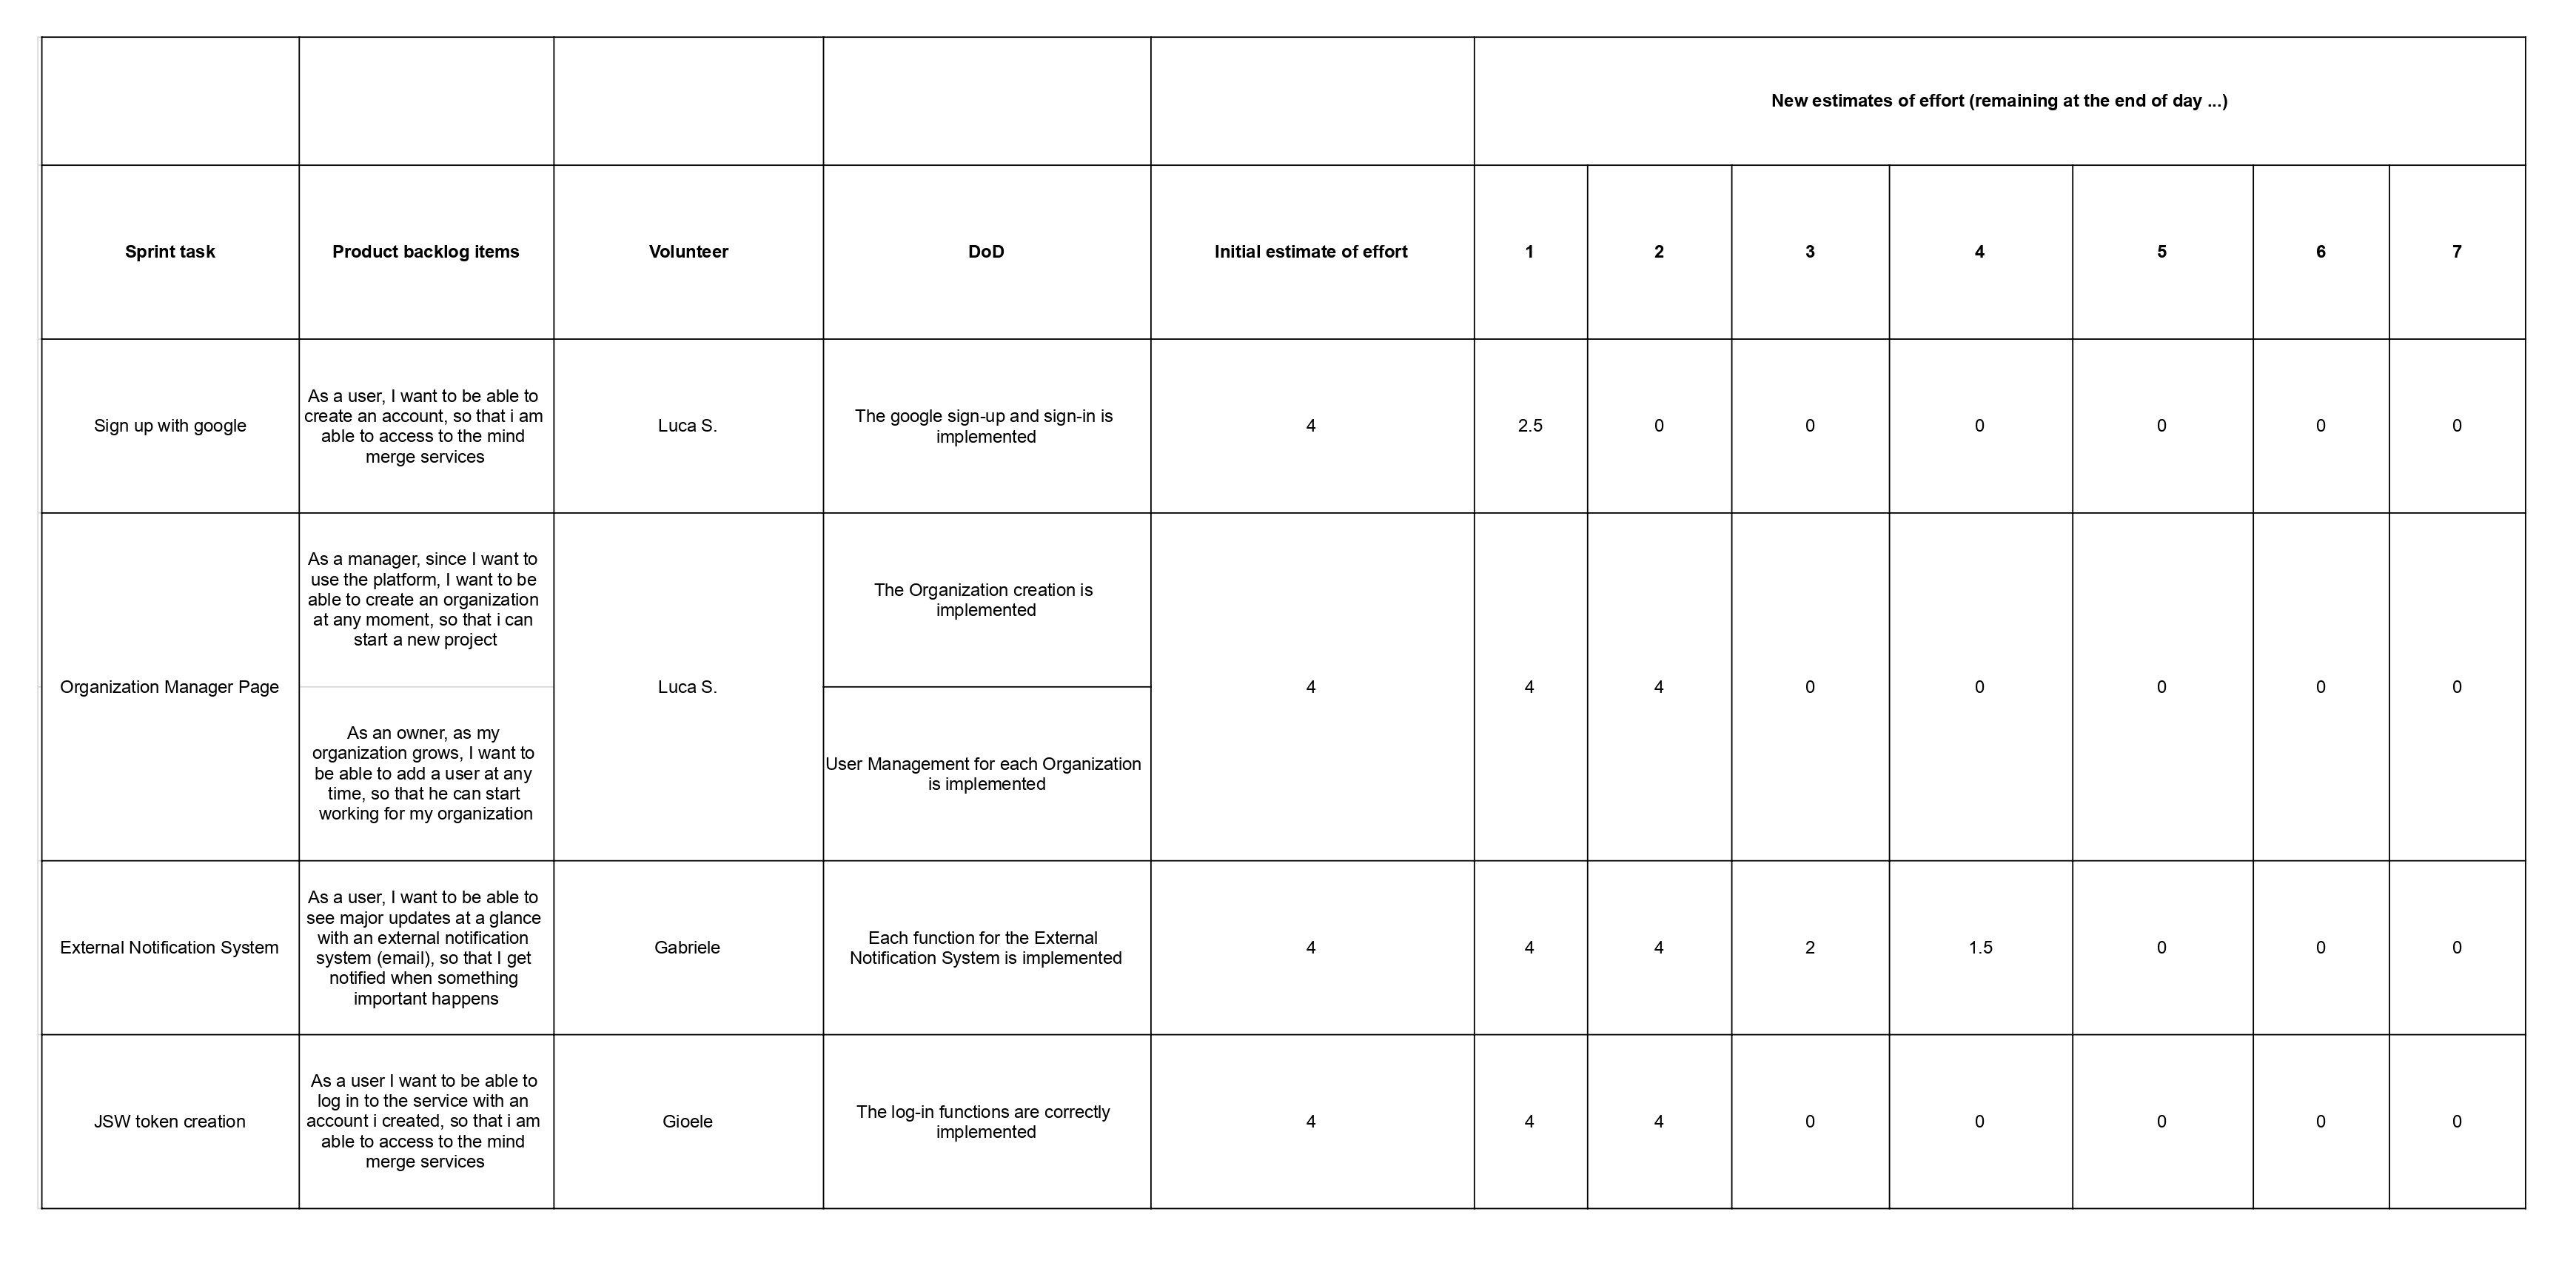
\includegraphics[width=0.95\textwidth]{images/sprint_backlog_2.jpg}

\subsection{Review and Retrospective}

\subsubsection{Retrospective}
Sprint 2 went well overall. However, as reflected in the burndown chart, we underestimated our velocity. This was primarily because we allocated a significant amount of time during the week for another course project that we anticipated would require considerable effort. To our surprise, we completed that project in one day, leaving us with more available time for the rest of the week.

Our main concern going into Sprint 3 is becoming more familiar with the Vue framework. By the end of Sprint 2, we still faced challenges in using it effectively.

\subsubsection{Review}
We demonstrated the Google sign-in functionality and the "Organization Manager" page to the product owner. This page allows users to create an organization and add or remove users.

The product owner was happy with the results but requested a change. Specifically, he asked that when a new organization is created, it should automatically be selected as the current active organization. We will note this down and address it in one of the upcoming sprints.
\subsection{Burn-down Chart}
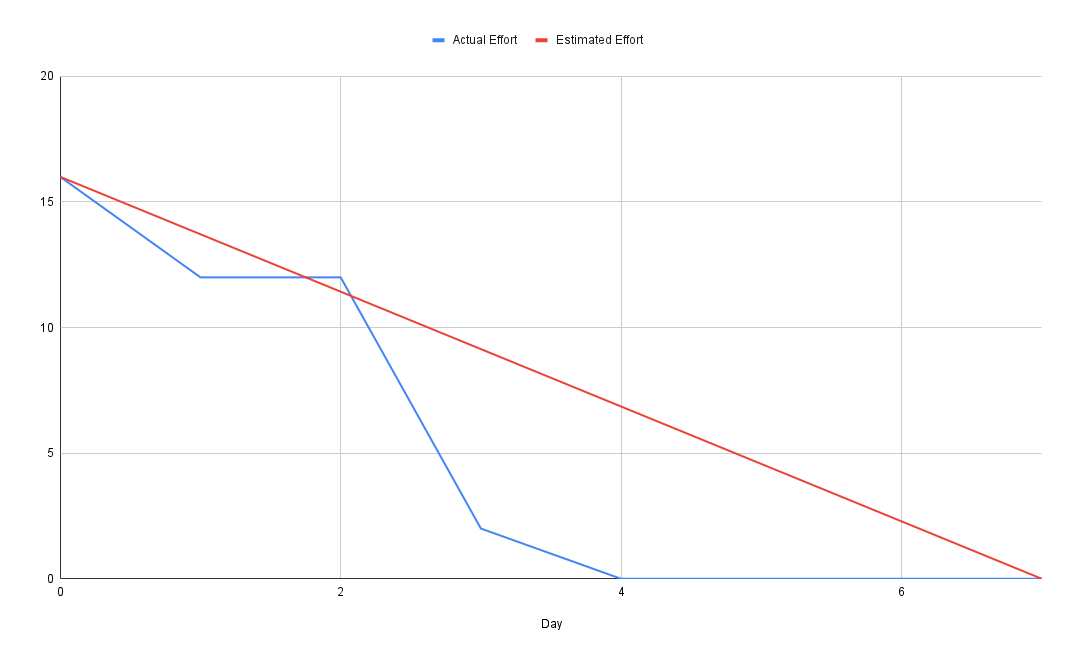
\includegraphics[width=0.95\textwidth]{images/burndown_chart_2.png}

\section{Sprint 3}

\subsection{Backlog}
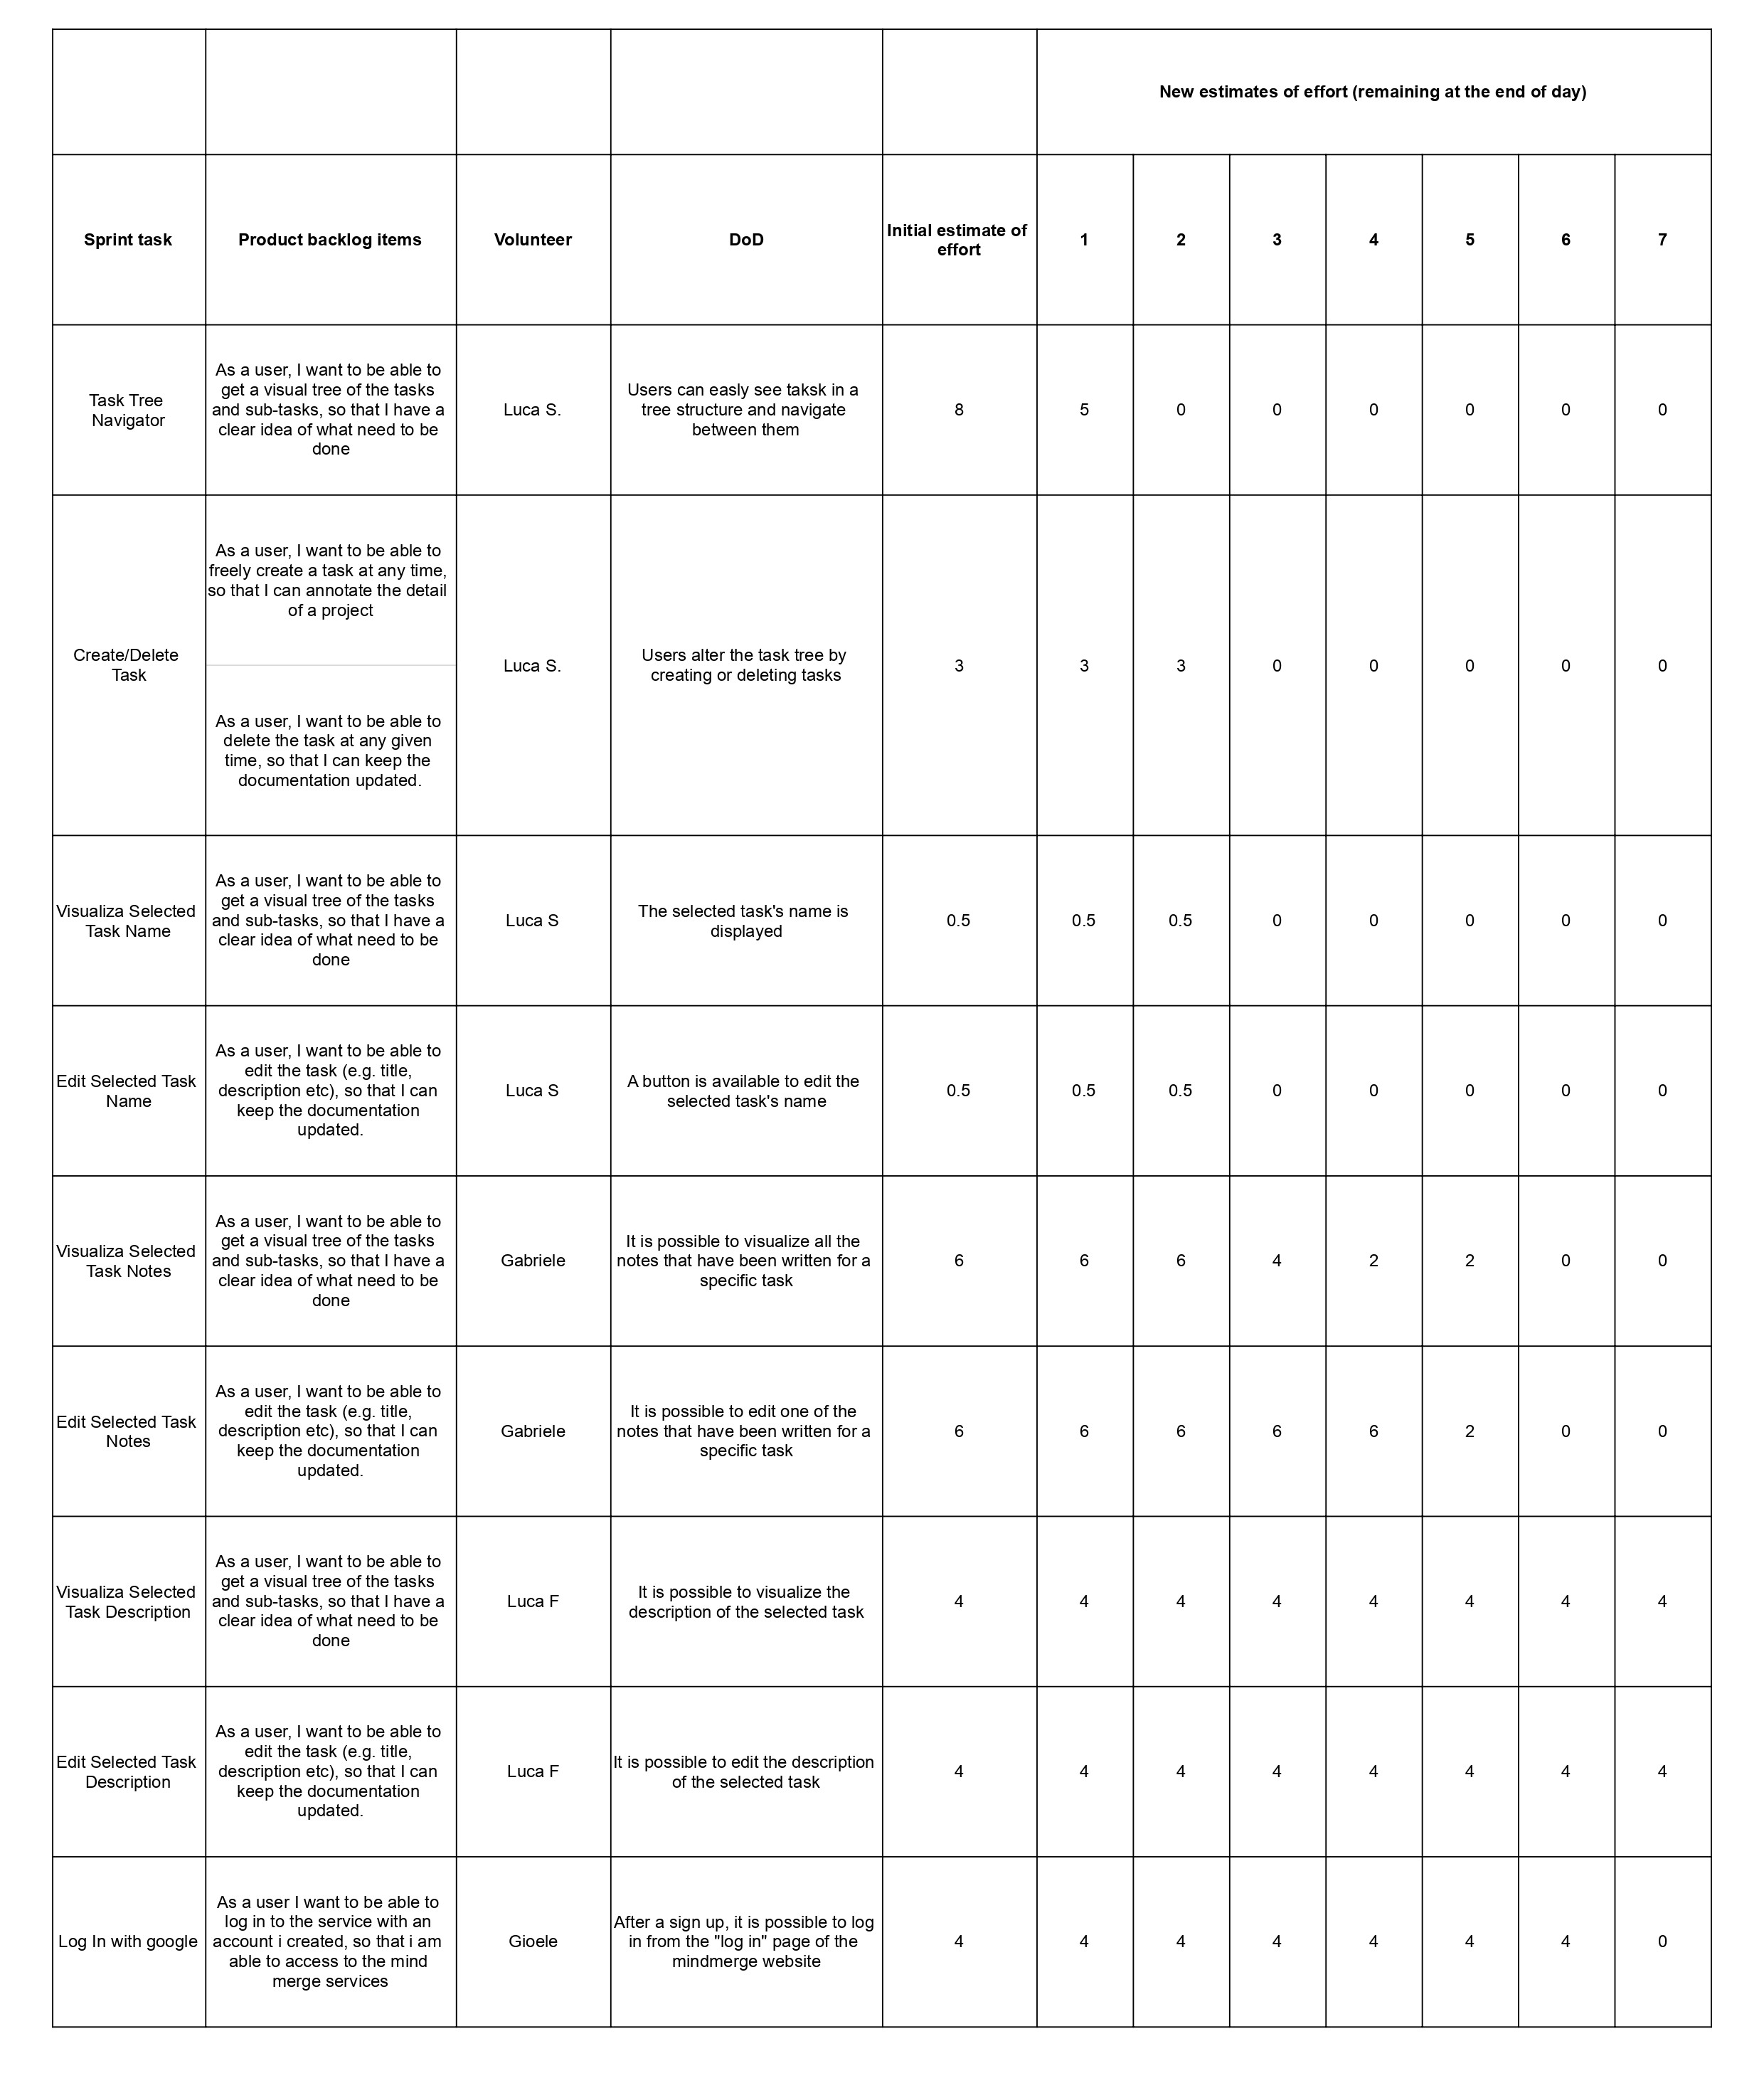
\includegraphics[width=0.95\textwidth]{images/sprint_backlog_3.jpg}

\subsection{Review and Retrospective}
\subsubsection{Retrospective}
In this sprint, we became more familiar with the Vue framework and managed to build the pages faster compared to the last sprint. We now feel proficient in the tooling and are hopeful for the completion of the project.

This time, we didn’t manage to complete every task. However, we came really close to completion. Considering that we had other midterm exams during the same week or the week after the sprint, we remain relatively happy with the results.
\subsubsection{Review}
The Product Owner liked the interface but found it annoying that when a new task was created, it needed to be selected manually. He asked us to change this.

He also noted that the task description was missing and requested its implementation as soon as possible.

Despite these minor inconveniences, he was happy with the result and told us that the page was really functional.
\subsection{Burn-down Chart}
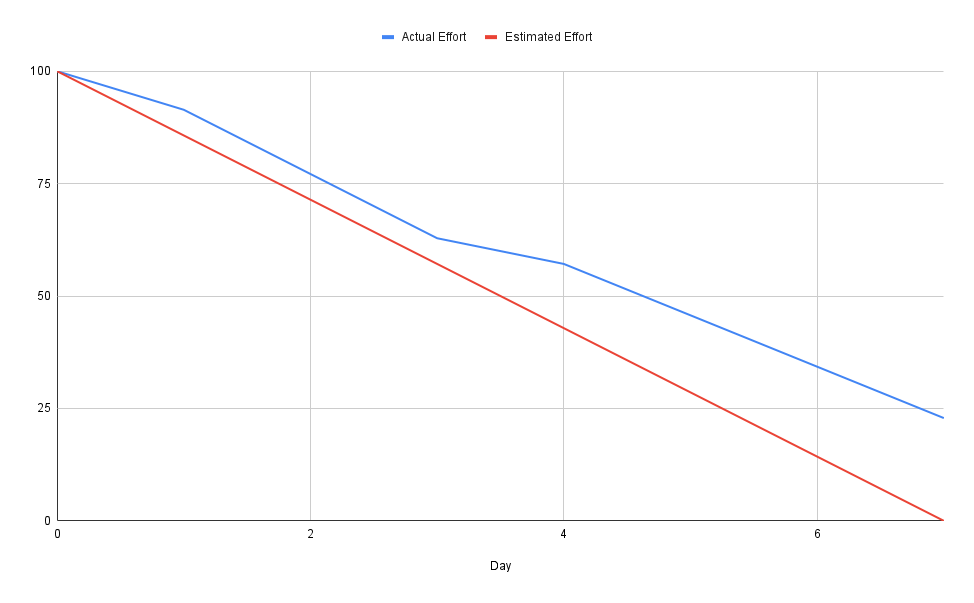
\includegraphics[width=0.95\textwidth]{images/burndown_chart_3.png}

\section{API Design and Documentation}
We have documented all of our APIs using the OpenAPI standard. The documentation is available at the following URL: \url{http://mindmerge-backend.onrender.com/api-docs}
\newline
Note that the documentation is hosted on Render; therefore, it may take a while to load the first time you access it, as mentioned in the limitations section.

\section{Testing Implementation}

At the end of our project, we implemented 70 automated tests, that can be run using the command \texttt{npm test}
in the backend folder.
\newline
The tests are also run automatically every time we push to the main branch, using GitHub Actions.

\subsection{Test Coverage}

With some approximations, we estimated that our tests cover about 70\% of the codebase.
\newline
Starting from the 183 tests that we defined at the beginning of the project, we subtract the 25 non-automated
tests that were defined, arriving at 158 automated tests.
\newline
From here we should subtract the 55 or so tests (depending on how you count them ) that
are testing feature that are not implemented yet. This leaves us with a total of 103 tests that should be implemented 
for a theoretical 100\% coverage.
\newline
Given that we have implemented 70 tests, we can estimate that we have a coverage of about 70\%.

\section{How to demo}
In this section We'll explain everything needed to demo and evaluate our project.
The first thing you should know is that you can access the frontend at the following URL: \url{https://lucasartore.github.io/MindMergeApp/sign_in}
\subsection{Demo Accounts}

To log in in the MindMerge account you'll need to use a Google account, that has been inserted in Google's developer console as a testing account.
This is because our app has not been published and verified by google, therefore there are some limitations on the accounts that can log in.

We have created two testing account, and we sent the credentials to you via email.
The email has been sent Monday 24th of June at 8:00 AM, with the subject ``MindMerge - Testing Account''.

If you prefer to use you own account, you can send us the email address you want to use, and we'll add it to the list of testing accounts.

\subsection{Demo Limitations}

Our demo has some minors limitations that stands from the fact that we are using a free tier of basically every service we are using.
We would like to quickly list them here so that you are aware of them before starting the demo.

\begin{itemize}
  \item \textbf{LLM Service:} We are using the free tear of the Google Bard API as our llm service. The free tear is limited to 15 requests per minute.
        One report generation uses as many requests as there are tasks in the task tree... This means that in one minute you can generate at most:
        \begin{itemize}
          \item 15 reports for a task that has no child tasks
          \item 5 reports for a task that has 3 child tasks
          \item 1 report for a task that has 15 child tasks
        \end{itemize}
        and so on...
  \item \textbf{Backend startup time:} The backend is hosted on render, with the free tear... this means that our service will be 
        shut down if it is not used for a while. According to the documentation this can ``delay requests by 50 seconds or more''.

        To quickly check whether the backend is up and running, you can go to the following URL: \url{https://mindmerge-backend.onrender.com/hello}
  \item \textbf{Backend response time:} As mentioned early we used the free google bard API, however the free tear is not available in the EU, therefore we
  had to position the the backend in the US, this makes the interface a bit slow, as every request made to the backend has to travel across the pacific ocean twice.

  \item \textbf{Notification email:} Our system will send you an email with a report every time you request it... however, we are using the free tear of the 
  services that allow us to send emails, therefore the emails will be sent from a random email address, and this makes it very likely that \textbf{the email will be marked as spam}.
\end{itemize}
\subsection{Video}
We have created a one minute pitch video that you can watch at the following URL: \url{https://youtu.be/GRvbIcb5EpE}

\subsection{Instructions}

\subsubsection{Refernece images}
In order to explain the functionalities of our application better, we created a few images that we will use to reference many UI elements.
\newline
\newline
\newline
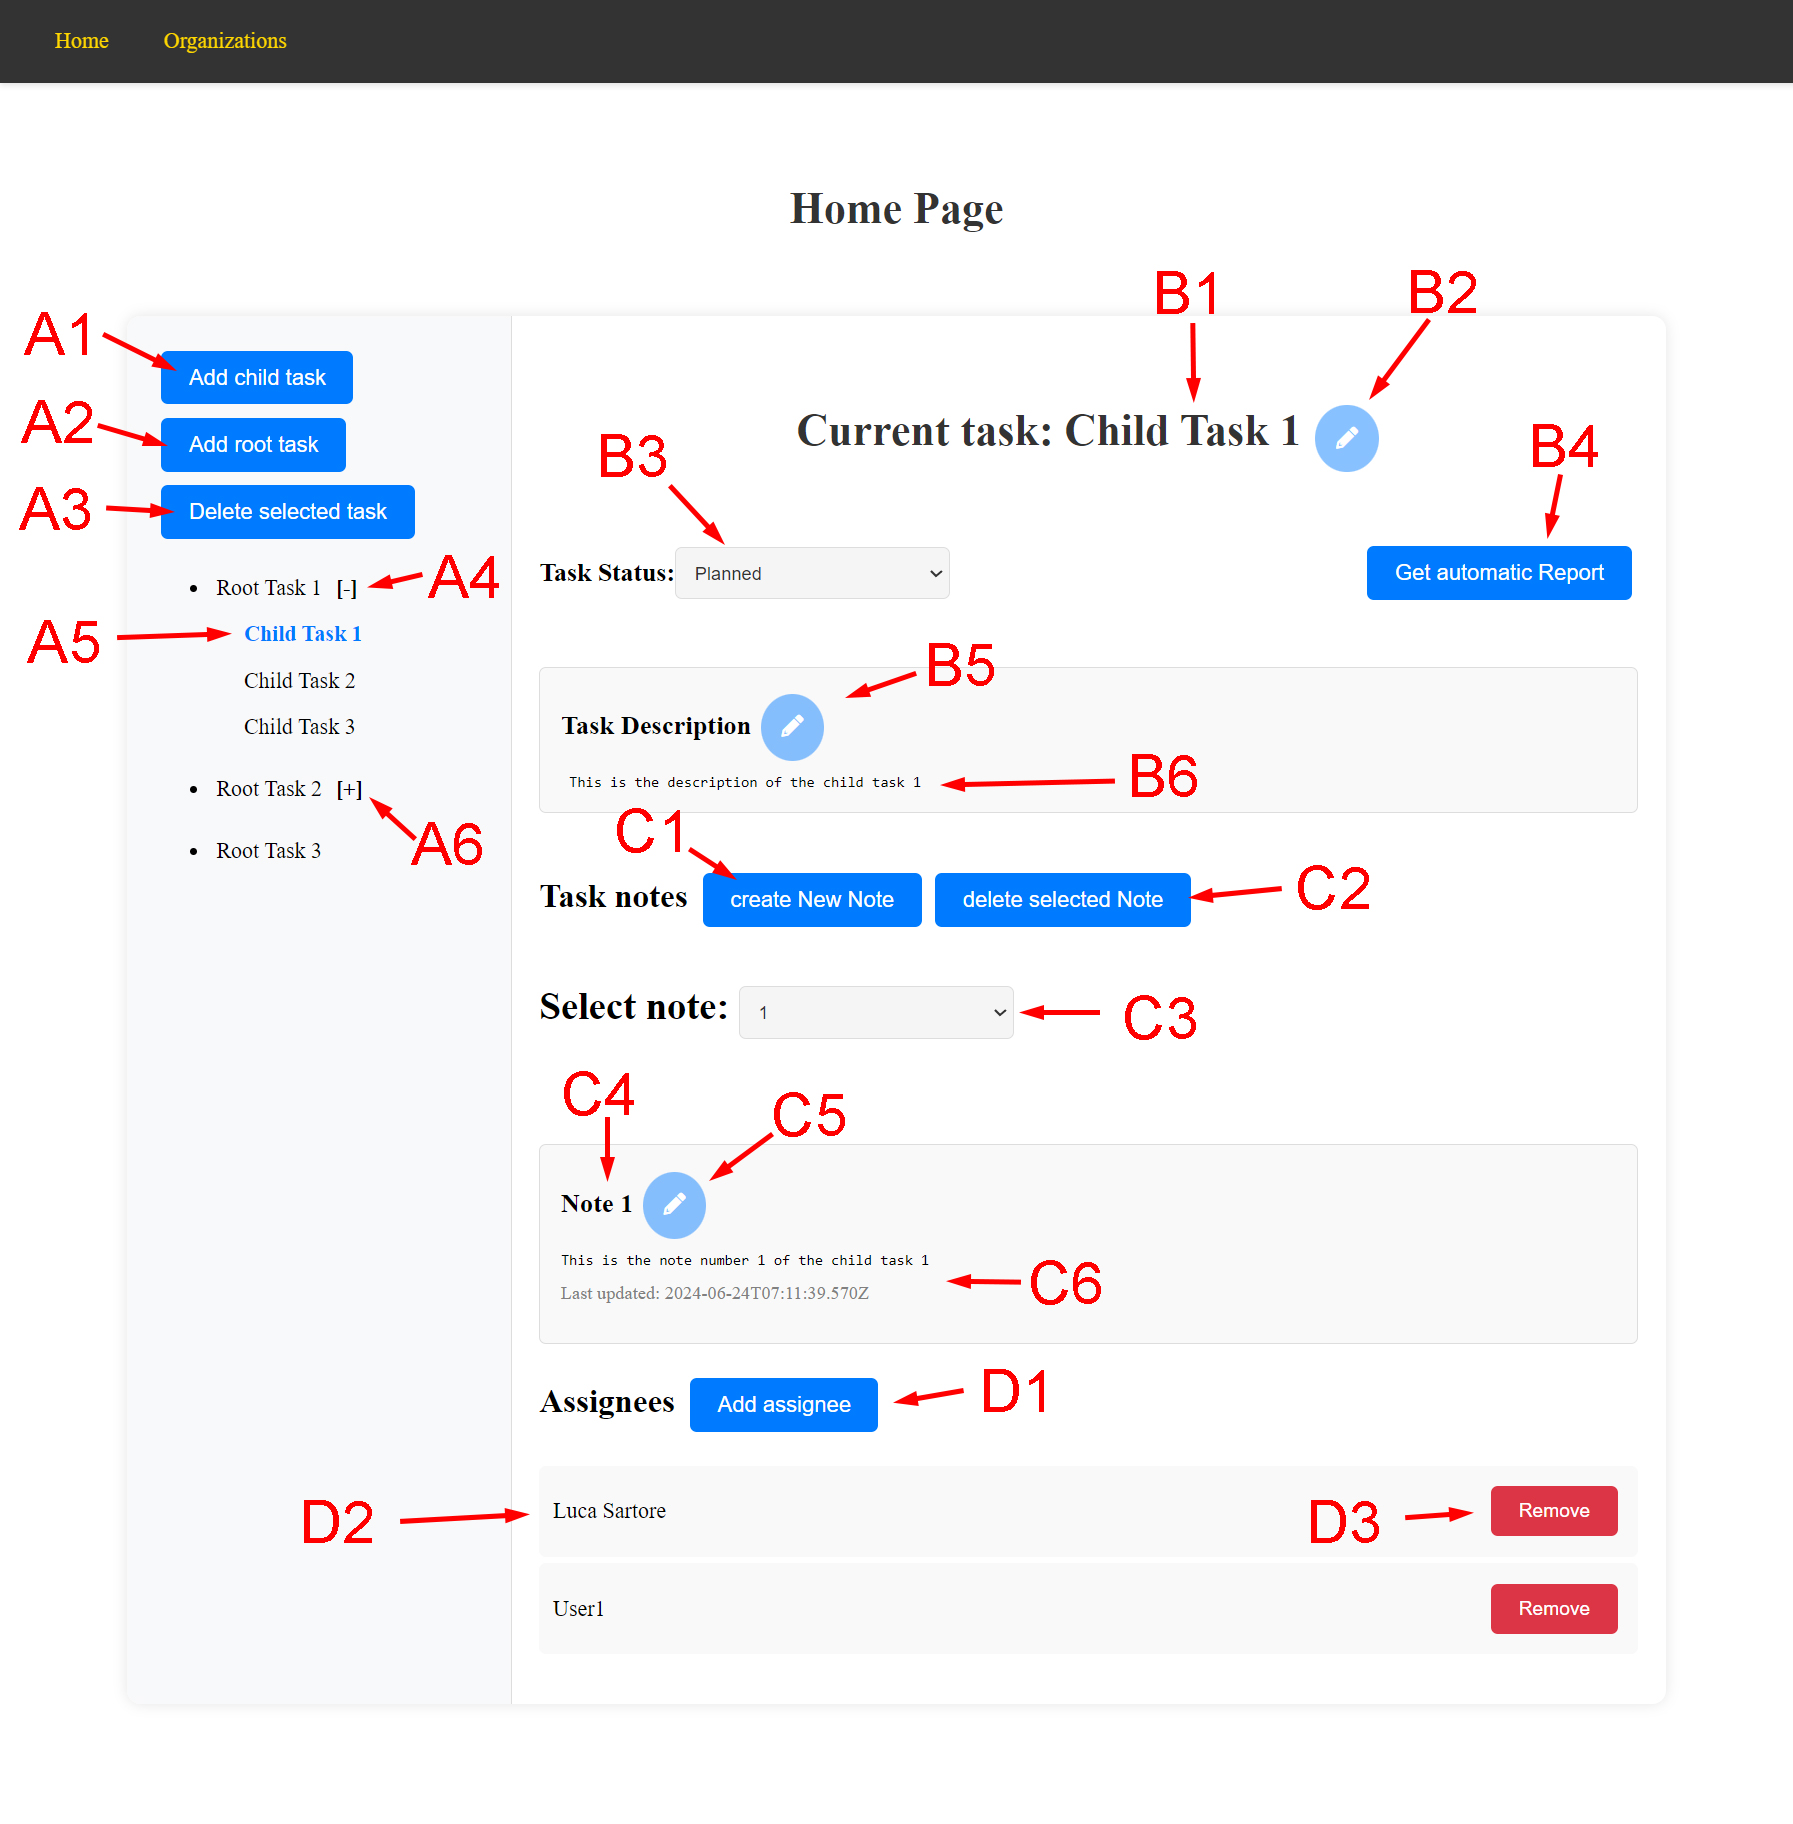
\includegraphics[width=0.95\textwidth]{images/home_page.jpg}
\newline
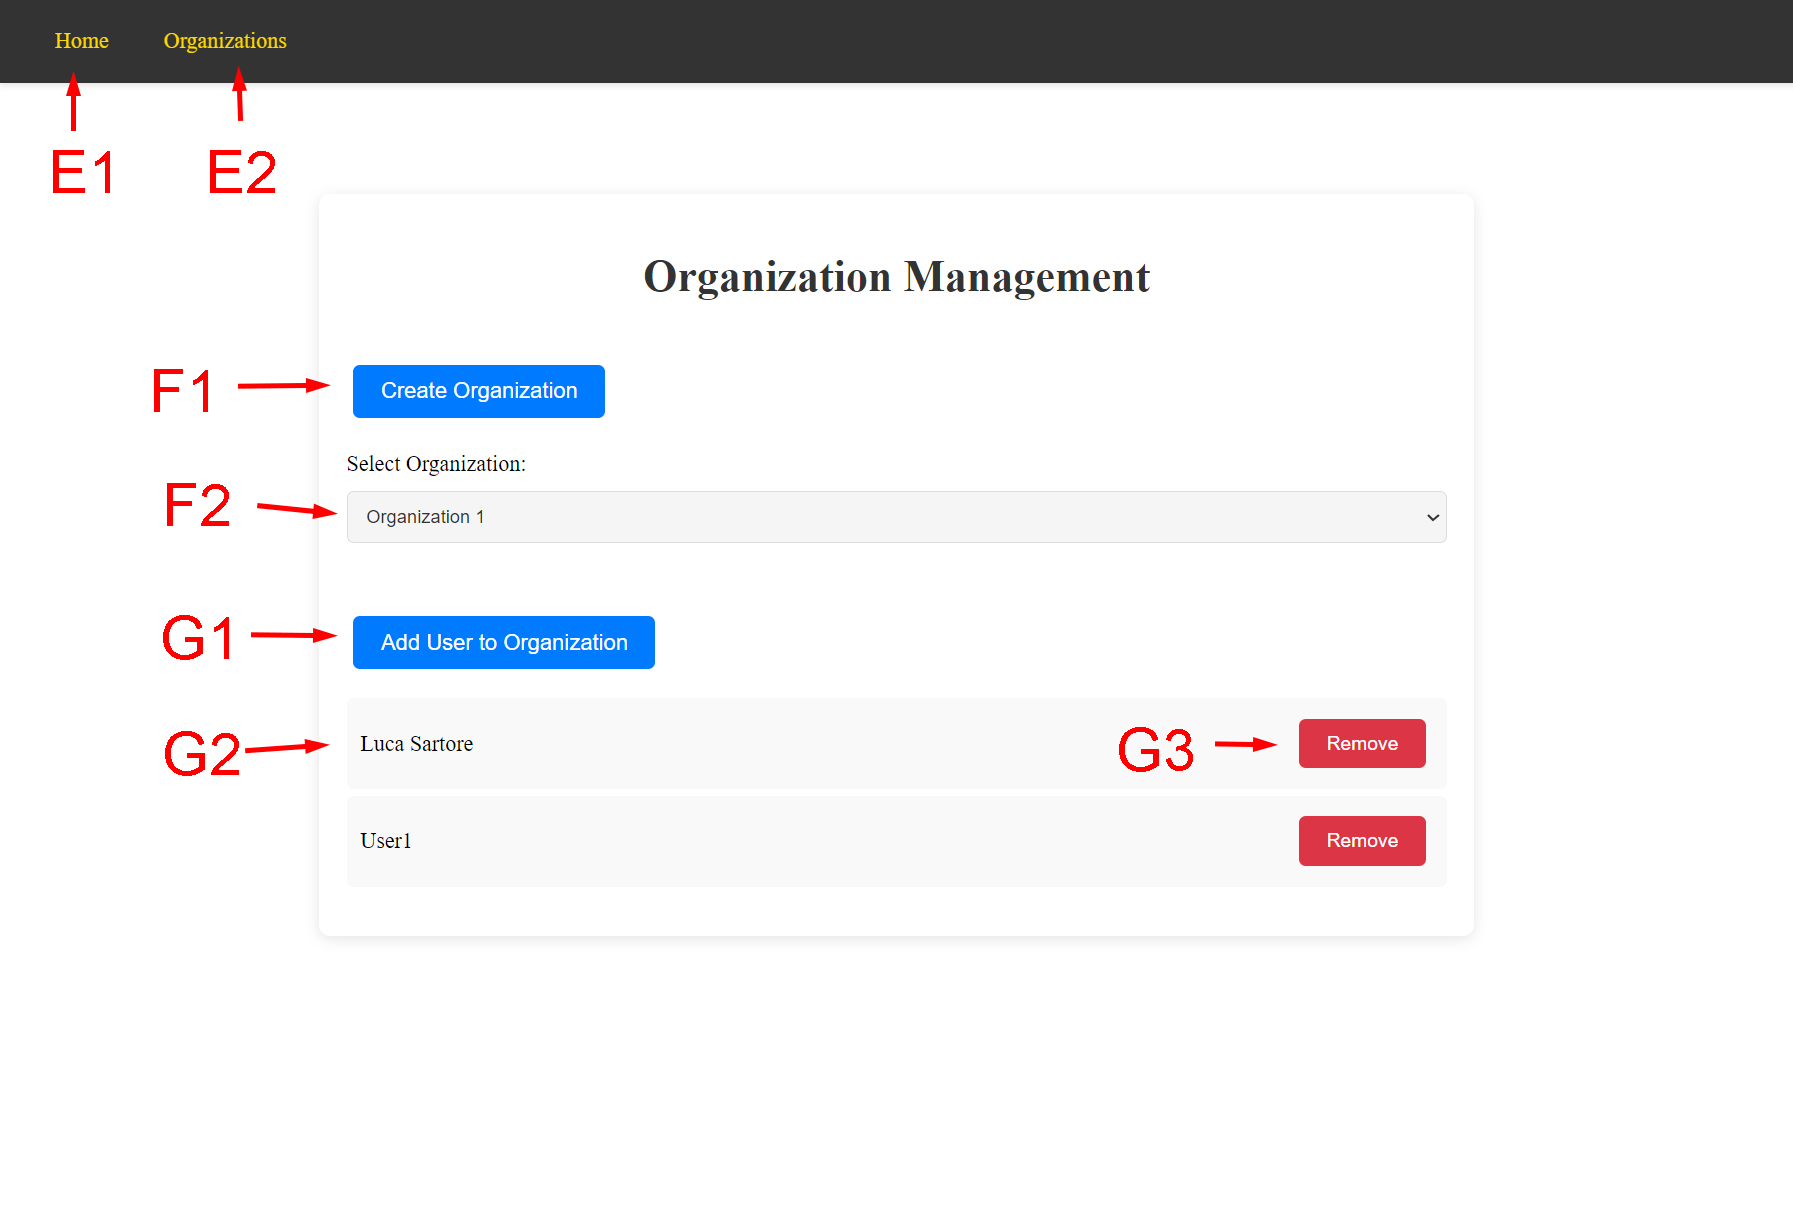
\includegraphics[width=0.95\textwidth]{images/organizations_page.jpg}

\subsubsection{Top bar}

The top bar is present on the top of every page, and allow the user to navigate between pages.
\newline
When the user is logged in, the top bar will show links to the home page \textbf{E1} and the organizations page \textbf{E2}.
You can click on the links to navigate to the respective pages.
\newline
When the user is not logged in it will show an about us section, a login section and a sign up section.

\subsubsection{Create organization}

To create an organization you need to click on the ``Create organization'' button \textbf{F1} on the organizations page \textbf{E2}.
After that you will be prompted to insert a name, and you should be able to create the organization by pressing ``ok''.
\newline
The organization selector \textbf{F2} allows the user to select the organization he wants to work on. By default
it will show the most recently created organization, and will automatically select an organization once it is created.

\subsubsection{Add user to organization}

By default the creator of an organization is the only member,
however he can add other users by pressing the ``Add user to Organization'' button \textbf{G1}.
After the button is pressed the user will be prompted to insert a unique user name (you can use ``MindMerge Tester1'' and ``MindMerge Tester2'' to test the feature).
\newline
Under the button you can see a list with all the users inside the organization \textbf{G2}.
as well as a button to remove them from the organization \textbf{G3}.
\subsubsection{Navigate task tree}
From the home page, you can navigate the task tree as well as creating new tasks.
\newline
You can click on a task name to visualize it's details, and when you do the selected task will be displayed in blue \textbf{A1}.
If a task has children it will display a small \textit{[+]} or \textit{[-]}
icon on the left of the name, that you can click to expand \textbf{A6} or collapse \textbf{A4} the children.

From this section you can also create and delete tasks; by using te buttons \textbf{A1, A2, A3}:
\begin{itemize}
  \item To create root task (a task that has no parent) you can click on the ``Add root task'' button \textbf{A2}.
  \item To create a child task you can click on the ``Add child task'' button \textbf{A1}. The new task will be created as a child of the selected task. 
  \item To delete the selected task you can click on the ``Delete taskTo delete the selected task you can click on the ``Delete task'' button \textbf{A3}.
Note that this will also delete all the children of the tasks.
\end{itemize}
\subsubsection{Edit task parameter}
From the top right area of the home page you have access to various task parameters that you can edit"
\begin{itemize}
  \item You can see the task's name \textbf{B1}.
  \item You can edit the task's name by clicking on the ``blue'' button \textbf{B2}.
  \item You can edit the task's status from the dropdown menu \textbf{B3}.
  \item You can ask a question that will be answered by an LLM using the ``Get automatic Report'' button \textbf{B4}.
  \item You can see the task's description \textbf{B6}.
  \item You can edit the task's description by clicking on the ``blue'' button \textbf{B5}.
\end{itemize}
\subsubsection{Edit task notes}

A task can also have some notes written by the users, to create, edit and delete notes you can use the following buttons:

\begin{itemize}
  \item To create a new note you can click on the ``create New Note'' button \textbf{C1}.
  \item In the ``Select note'' dropdown menu \textbf{C3} you can see all the notes that are associated with the task, and select
  the one you want to display.
  \item You will see the selected note's number in bold text \textbf{C4}; As well as the
  note's contend, and last edit date below \textbf{C6}.
  \item You can edit the note's content by clicking on the ``blue'' button \textbf{C5}.
  \item You can delete the note by clicking on the ``delete selected Note'' button \textbf{C2}.
\end{itemize}

\subsubsection{Edit task assignees}

To keep track of who is working on a task, you can assign users to it.
This is done by using the following buttons:
\begin{itemize}
  \item To assign a user to the task you can click on the ``Assign assignee'' button \textbf{D1}; And then insert the user's name.
  Remember that the user must be part of the organization to be assigned to a task.
  \item You will see the list of assignees below the button \textbf{D2}.
  \item You can remove an assignee by clicking on the ``Remove'' button \textbf{D3} to the right of the name.

\end{itemize}
\subsection{Testing automatic report}

To test the automatic report management feature you can use the organization named: ``Commissione Feste Universitarie (CFU)''
of which both MindMerge Tester1 and MindMerge Tester2 are members.
There you can find many preloaded tasks with description and notes that you can query.
We would appreciate if you could avoid editing this organization, as we would like to keep it as a demo.


You should know that when you ask a report it will start from the task that was selected when you pressed the button.
The LLM will have access to the informations of all the tasks that are below the selected task in the tree, but not to the informations of the tasks that are above it.
\newline
However it should be noted that obviously the answer will be more precise if you identify the correct task to start from.
\newline
A few questions you can ask are:
\begin{itemize}
  \item ask ``Summarize what this task is about?'' from the task ``Organize a new event in povo''
  \item ``Do We already have a structure for the event?'' from the task ``Organize a new event in povo'' or the task ``Ask for structure availability''
  \item ``Where haven't we placed posters so far?'' from the task ``Stick posters around''
\end{itemize}

\subsection{Error handling}

To test our frontend error handling you can generate an error by doing one of two things:
\begin{itemize}
  \item You can try to delete the organization owner (that is the first name in the list of members) from the organization.
  \item You can load a task and start edit the title, then you can log in with another account and delete, and then try to complete 
  the title editing.
\end {itemize}

Both of these actions will generate an error, and the user will see an alert with the error message.

\end{document}